\documentclass[
    12pt, % Schriftgröße
    DIV=10,
    a4paper, % Papierformat
    oneside, % einseitiges Dokument
    titlepage, % es wird eine Titelseite verwendet
    parskip=half, % Abstand zwischen Absätzen (halbe Zeile)
    headings=normal, % Größe der Überschriften verkleinern
    listof=totoc, % Verzeichnisse im Inhaltsverzeichnis aufführen
    bibliography=totoc, % Literaturverzeichnis im Inhaltsverzeichnis aufführen
    captions=tableheading, % Beschriftung von Tabellen unterhalb ausgeben
    numbers=noendperiod 	% kein Punkt nach Nummerierung in Überschrift
]{scrreprt}


\usepackage[
    automark,       % Kapitelangaben in Kopfzeile automatisch erstellen
    headsepline,    % Trennlinie unter Kopfzeile
    footsepline,
    ilines          % Trennlinie linksbündig ausrichten
]{scrpage2}

\usepackage[section]{placeins}
\usepackage[ngerman]{babel}
\usepackage[utf8]{inputenc}
\usepackage[T1]{fontenc}
\usepackage{pdfpages}

\usepackage{setspace}
\onehalfspacing % Zeilenabstand 1,5 Zeilen

\usepackage{geometry}
\setlength{\topskip}{\ht\strutbox} % behebt Warnung von geometry
\geometry{left=35mm,right=30mm,top=25mm,bottom=45mm}

% Kopf- und Fußzeilen
\pagestyle{scrheadings}
% Kopf- und Fußzeile auch auf Kapitelanfangsseiten
\renewcommand*{\chapterpagestyle}{scrheadings} 
% Schriftform der Kopfzeile
\renewcommand{\headfont}{\normalfont}

% Kopfzeile
%\ihead{\large{\textsc{\titel}} \\[2ex] \textit{\headmark}}
\ihead{\large{} \\[2ex] \textit{\headmark}}
\chead{}
\ohead{
\includegraphics[scale=0.12]{\logo} \hspace*{25mm}}
\setlength{\headheight}{21mm} % Höhe der Kopfzeile
% Kopfzeile über den Text hinaus verbreitern
\setheadwidth[0pt]{textwithmarginpar} 
\setheadsepline[text]{0.4pt} % Trennlinie unter Kopfzeile

% Fußzeile
\ifoot{\autor}
\cfoot{}
\ofoot{\pagemark}


\usepackage{courier}
\usepackage{relsize} 
\usepackage{graphicx}
\usepackage{amsmath,amsfonts}
\usepackage{longtable}
\usepackage{mathtools}
\usepackage{eurosym}

\usepackage{booktabs}
\usepackage{xcolor}
\usepackage{rotating,tabularx}

\usepackage{tablefootnote}

\usepackage{hhline}
\usepackage{array}
\newcolumntype{C}[1]{>{\centering\let\newline\\\arraybackslash\hspace{0pt}}m{#1}}   % center
\newcolumntype{L}[1]{>{\raggedright\let\newline\\\arraybackslash\hspace{0pt}}m{#1}} % left
\newcolumntype{R}[1]{>{\raggedleft\let\newline\\\arraybackslash\hspace{0pt}}m{#1}}  % right
\newcolumntype{w}[1]{>{\raggedleft\hspace{0pt}}p{#1}}


\usepackage{paralist} % Formatierung von Listen ändern
\usepackage{todonotes}
% usage: \todod{Adressat}{Frage}
\newcommand{\mytodo}[2]{
    \IfEqCase{#1}{
        {Steff}{\todo[color=orange]{#1}{\textit{#2}}}
        {Hofmann}{\todo[color=yellow]{#1}{\textit{#2}}}
        {cite}{\todo[color=blue]{#1}{}}
        {rework}{\todo[color=pink]{#1}{}}
        {}{\todo[color=green]{#1}{\textit{#2}}}
    }[\PackageError{mytodo}{Undefined option to todod: #1}{}]
}


\usepackage[printonlyused]{acronym}

\usepackage{chronology}
\usepackage{tikz}
\usepackage{pgfplots}
\usepackage{numprint}
\pgfplotsset{compat=1.14} 
\usepackage{mathptmx}
\usepackage{calc}
\usepackage{xcolor} 

\usepackage[toc]{glossaries}
\loadglsentries{nebenkapitel/Glossar}
\makeglossaries
\glsaddall{}

\usepackage{pifont}
\newcommand{\cmark}{\textcolor[rgb]{0,0.6,0}{\ding{51}}}
\newcommand{\xmark}{\textcolor{red}{\ding{55}}}

\newcommand*{\TakeFourierOrnament}[1]{{\fontencoding{U}\fontfamily{futs}\selectfont\char#1}}
\newcommand*{\danger}{\textcolor[RGB]{255,200,0}{\TakeFourierOrnament{66}}}

\frenchspacing % erzeugt ein wenig mehr Platz hinter einem Punkt

% Schusterjungen und Hurenkinder vermeiden
\clubpenalty = 10000
\widowpenalty = 10000 
\displaywidowpenalty = 10000

\usepackage{floatflt}
\usepackage{minted}
\usepackage{listings}
\definecolor{myblue}{RGB}{5, 79, 114}
\definecolor{mybluelight}{RGB}{9, 132, 191}
\definecolor{myblueextralight}{RGB}{0, 155, 210}
\definecolor{greendark}{RGB}{0, 153, 51}
\definecolor{colBackground}{RGB}{240, 240, 240}
\definecolor{colKeys}{RGB}{0, 0, 255}
\definecolor{colIdentifier}{RGB}{0, 0, 0}
\definecolor{colComments}{RGB}{40, 220, 0}
\definecolor{colString}{RGB}{0, 150, 0}
\lstset{
    float=hbp,
    basicstyle=\ttfamily\color{black}\small\smaller,
    identifierstyle=\color{colIdentifier},
    keywordstyle=\color{colKeys},
    stringstyle=\color{colString},
    commentstyle=\color{colComments},
    columns=flexible,
    tabsize=2,
    frame=single,
    extendedchars=true,
    showspaces=false,
    showstringspaces=false,
    numbers=left,
    numberstyle=\tiny,
    numbersep=5pt,
    breaklines=true,
    backgroundcolor=\color{colBackground},
    emph={square}, 
    emphstyle=\color{red}, 
    emph={[2]root,base}, 
    emphstyle={[2]\color{blue}},
    breakautoindent=true
}


\usepackage[
    bookmarks,
    bookmarksopen=true,
    colorlinks=true,
    linkcolor=black,
    anchorcolor=black,
    citecolor=black,
    filecolor=black,
    menucolor=black,
    urlcolor=black, 
    %backref,
    plainpages=false,
    pdfpagelabels,
    hypertexnames=false
]{hyperref}


% Abkürzungen mit korrektem Leerraum 
\newcommand{\ua}{\mbox{u.\,a.\ }}
\newcommand{\zB}{\mbox{z.\,B.\ }}
\newcommand{\vgl}{vgl.\ }
\newcommand{\bzw}{bzw.\ }
\newcommand{\evtl}{evtl.\ }
\newcommand{\ggf}{ggf.\ }
\newcommand{\usw}{usw.\ }
\newcommand{\etc}{etc.\ }
\newcommand{\idR}{i.\,d.\,R.\ }
\newcommand*\NewPage{\newpage\null\thispagestyle{empty}\newpage}

\newcommand{\bs}{$\backslash$}
\newcommand{\arrow}{$\to$}

% Listenelement mit fetter Überschrift und Zeilenumbruch -> \itemd{Überschrift}
\newcommand{\itemd}[1]{\item{\textbf{#1}}\\}

\newcommand{\textcour}[1]{
    \begin{footnotesize}
        \texttt{#1} 
    \end{footnotesize}
}

% Tabelleninhalte werden grundsätzlich in kleinerer Schriftgröße erstellt
\usepackage{etoolbox}
\AtBeginEnvironment{tabular}{\footnotesize}


\newcommand{\titel}{Entwurf und Implementierung eines Conversational User Interfaces für das Bankkontenmanagement mit Alexa Voice Services}
\newcommand{\art}{Masterarbeit}
\newcommand{\fachgebiet}{Software-Engineering}
\newcommand{\autor}{Julian Wölk}
\newcommand{\studienbereich}{Elektronische und Mechatronische Systeme}
\newcommand{\vertiefung}{Informationstechnik}
\newcommand{\matrikelnr}{2273025}
\newcommand{\erstgutachter}{Prof. Dr. Oliver Hofmann}
\newcommand{\zweitgutachter}{Prof. Dr. Matthias Hopf}
\newcommand{\betreuer}{Dipl.-Inf. Steffen Blümm}
\newcommand{\jahr}{2017}
\newcommand{\ort}{Nürnberg}
\newcommand{\logo}{bilder/LogoOhmHochschule.jpg}
\newcommand{\hs}{Technische Hochschule Nürnberg Georg Simon Ohm}
\newcommand{\adorsys}{adorsys GmbH \& Co. KG}

\begin{document}

% auch subsubsection nummerieren
\setcounter{secnumdepth}{3}
\setcounter{tocdepth}{3}

% Deckblatt und Abstract ohne Seitenzahl
\ofoot{}
\NewPage
\thispagestyle{plain}
\begin{titlepage}

\advance\leftskip-1cm 
\includegraphics[scale=.7]{bilder/LogoTHMitText.jpeg} \hfill \advance\rightskip-1cm  
\includegraphics[scale=.017]{bilder/logo.png}\\[12ex]

\begin{center}
    %
\includegraphics[scale=1.1]{bilder/LogoTHMitText.jpeg}\\[11ex]  
    
    \huge{\textbf{\titel}}\\[6.5ex] 
    \LARGE{\textbf{\art}}\\[1.5ex]
    
    \normalsize
    \begin{tabular}{w{5.4cm}p{7cm}}\\
    vorgelegt von:  & \quad \textbf{\autor}\\[1.2ex]
    Studiengang: & \quad \studienbereich\\[1.2ex]
    Vertiefungsrichtung: & \quad \vertiefung\\[1.2ex]
    Erstgutachter:  & \quad \erstgutachter\\[1.2ex]
    Zweitgutachter: & \quad \zweitgutachter\\[1.2ex]
    Betreuer: & \quad \betreuer\\[3ex]
    \end{tabular}
    
    WiSe 2017/2018\\[6ex]
    Schlagworte: Voice User Interface, Conversational User Interface, Amazon Alexa, CUI Prototyping
\end{center}
\end{titlepage}

\section*{Abstract}
\label{sec:zusammenfassung}
Mit der Veröffentlichung von \textit{Siri} im Jahr 2011 leitet \textit{Apple} eine neue Generation von \textit{\acp{VUI}} ein. Sprach- und textgesteuerte Assistenten gewinnen seitdem an Beliebtheit.\\ 
Auch wenn die Idee nichts neues ist, hat die zunehmende Rechenleistung ermöglicht, dass diese neuen Schnittstellen mit natürlicher Sprache verwendet werden können. Das lässt auf großes Potenzial in vielen Anwendungsbereichen schließen, darunter auch der Finanzsektor. Gerade als persönlicher Assistent gewährt ein solches \ac{VUI} schnellen Zugriff auf Informationen. Antworten müssen nicht mehr gesucht, sondern können direkt erfragt werden. Da sie auf natürliche Sprache reagieren, ist es theoretisch auch nicht mehr nötig, die Sprachbefehle für die Interaktion zu kennen. Jedoch verstehen diese Technologien nur soviel, wie man ihnen beibringt. Damit sie im Stande sind, echte konversationsnahe Unterhaltungen zu führen, müssen sie dementsprechend entwickelt werden. Weg vom einfachen Frage-Antwort \textit{Voice User Interface}, hin zum \textit{\ac{CUI}}.\\
Die Arbeit umfasst zum einen die Konzeption eines solchen Systems. Es wird festgestellt, welche Anforderungen an ein \ac{CUI} im Allgemeinen und an eine entsprechende Anwendung für das Bankkonten-Management gestellt werden. Um das zu erreichen, werden Paradigmen und Methoden aus dem Bereich des \textit{Usability Engineering} angewandt. Im Zuge dessen wurde auch eine Prototyping Toolchain für \acp{CUI} entwickelt. Zum anderen soll auf Basis dessen ein prototypisches System mit \textit{Amazon Alexa} \cite{amazon-developer-alexa} umgesetzt werden.\\
Das Ziel der Arbeit ist festzustellen, welche der Anforderungen mit dem entwickelten Prototypen zufriedenstellend erfüllt werden können. Bei der Umsetzung wurde nicht das von Amazon bereitgestellte \ac{SDK} \cite{alexa-sdk} verwendet, sondern eine eigene Lösung erarbeitet. Implementiert wurden dabei die eigentliche Anwendung (Alexa Skill), ein Backend mit angebundener Datenbank und eine Smartphone-Anwendung. Der Skill, das Backend und die Datenbank wurden über externe Server bereitgestellt. Benutzer können in Verbindung mit einem Alexa Endgerät und der entwickelten App die implementierten Funktionen für fiktive Konten nutzen. Dabei wurden für den Prototypen das Abfragen des Kontostandes und die Durchführung von Transaktionen umgesetzt. 
\ofoot{\pagemark}

\pagenumbering{Roman}
\tableofcontents            % Inhaltsverzeichnis

\chapter*{Abkürzungsverzeichnis}			% keine Kapitelnummer -> section*
\addcontentsline{toc}{chapter}{Abkürzungsverzeichnis}
\markboth{Abkürzungsverzeichnis}{Abkürzungsverzeichnis}

\begin{acronym}[Bash]
	
	%%% A - E %%%
	\acro{AI}{Artificial Intelligence}
	\acro{ASK}{Alexa Skills Kit}
	\acro{ASR}{Automatic Speech Recognition}
	\acro{AVS}{Alexa Voice Service}
	\acro{AWS}{Amazon Web Services}
    
    \acro{BIC}{Bank Identifier Code}
    
    \acro{cft}{communication flow tool}
    \acro{cpt}{communication prototyping tool}
    \acro{CRUD}{Create-Read-Update-Delete}
    \acro{CUI}{Conversational User Interface}
    
    %%% F - J %%%
    \acro{FaaS}{Function as a Service}
	
	\acro{GUI}{Graphical User Interface}
	
	\acro{HiFi}{High-Fidelity}
	
	\acro{IBAN}{International Bank Account Number}
	\acro{IP}{Internet Protocol}
	\acro{IVR}{Interactive Voice Response}
	
	\acro{JSON}{JavaScript Object Notation}
	\acro{JS}{JavaScript}
	
	%%% K - O %%%
	\acro{KI}{Künstliche Intelligenz}
	
	\acro{LoFi}{Low-Fidelity}
	
	\acro{MiFi}{Mid-Fidelity}
	\acro{ML}{Machine Learning}
	
	\acro{NLP}{Natural Language Processing}
	\acro{npm}{Node Package Manager}
	
	\acro{ORM}{Object Relational Mapping}
	
	%%% P - T %%%
	\acro{prt}{phrase render tool}
	
	\acro{REST}{Representational State Transfer}
	
	\acro{SDK}{Software Development Kit}
	\acro{SQL}{Structured Query Language}
	\acro{SSL}{Secure Sockets Layer}
	
	\acro{TAN}{Transaction Authentication Number}
	\acro{TLS}{Transport Layer Security}
	\acro{TS}{TypeScript}
	\acro{TTS}{Text-To-Speech}
	
	%%% U - Z %%%
	\acro{URL}{Uniform Resource Locator}
	\acro{UUID}{Universally Unique Identifier}
	
	\acro{VM}{Virtual Machine}
	\acro{VoIP}{Voice over IP}
	\acro{VUI}{Voice User Interface}
	
	\acro{WOz}{Wizard-of-Oz}
    
\end{acronym}

\clearpage
      % Abkürzungsverzeichnis
%\clearpage\markboth{\nomname}{\nomname} % für korrekte Überschrift in der Kopfzeile
%\printnomenclature


\listoffigures              % Abbildungsverzeichnis
\listoftables               % Tabellenverzeichnis

\renewcommand{\lstlistlistingname}{Quellcodeverzeichnis}
\lstlistoflistings          % Quellcodeverzeichnis

\clearpage
\pagenumbering{arabic}

\chapter{Einleitung}
\label{cha:einleitung}

Wird bei bestimmten Begriffen, die sich auf Personengruppen beziehen, nur die männliche Form gewählt, so ist dies nicht geschlechtsspezifisch gemeint, sondern geschah ausschließlich aus Gründen der besseren Lesbarkeit.

\section{Motivation}
\label{sec:motivation}

\textit{Technologien sind Ressourcen, zu denen ein Interface den Zugang verschafft} \cite{cui-future-interface}. Anders als das \textit{\ac{GUI}}, ermöglicht ein \textit{\ac{CUI}} diesen Zugang nicht nur durch grafische Unterstützung, sondern hauptsächlich über Sprach"~ \bzw Texteingaben. Ein weiterer entscheidender Aspekt, den es mit sich bringt, ist Intelligenz. Es ist nicht nur ein Kommandozeilen"~ Interface. Vielmehr werden diese Technologien mit dem Verständnis für den entsprechenden Nutzungskontext gekoppelt. Während also über ein \ac{GUI} die Antwort auf eine Frage gesucht werden muss, kann man einem \ac{CUI} die Frage schlichtweg stellen und erhält die entsprechende Antwort. 

Es gibt verschiedene Ausprägungen von \acp{CUI}. Zum einen \textit{Chatbots}, welche primär mit eingegebenen Text interagieren. Zum anderen \textit{\acp{VUI}}, die über Spracheingaben bedient werden können. 

Hierzu zählen auch Sprachassistenten wie \textit{Apple Siri}\footnote{https://www.apple.com/ios/siri/, Abgerufen 31.10.2017} und \textit{Samsung S- Voice}\footnote{http://www.samsung.com/global/galaxy/what-is/s-voice/, Abgerufen 31.10.2017}. Diese sind vor allem durch mobile Endgeräte bereits weit verbreitet. Sie erleichtern seit Jahren die Bedienung und die Ausführung diverser Aufgaben. Auch \textit{Amazon}\footnote{https://www.amazon.de, Abgerufen 31.10.2017} hat ein solches System entwickelt. Der \textit{\ac{AVS}} \cite{amazon-developer-alexa} wurde Ende 2014 in Verbindung mit der passenden Hardware, dem \textit{Amazon Echo} \cite{amazon-echo}, veröffentlicht. Dieser verbindet sich bei Spracheingabe über das Internet mit dem AVS. Gesprochenes wird verarbeitet und die Antwort über den Lautsprecher des Echo Gerätes wieder ausgegeben. Der Umfang des Sprachverständnisses ist durch Anwendungen, den sogenannten \textit{Skills}, definiert. Dabei ist es auch möglich eigene Skills zu implementieren, um den Funktionsumfang zu erweitern. 
Ein Bereich, der für Sprachassistenten viele Anwendungsmöglichkeiten bietet, ist der Finanzsektor. Hier könnten eingesetzte \acp{CUI} viele Prozessabläufe für Banken und deren Kunden vereinfachen. Neben der Neueröffnung eines Kontos, der Durchführung eines Beratungsgespräches und dem Bestellen einer neuen Kredit"~ \bzw EC Karte, wäre auch eine sprachgesteuerte Verwaltung von Bankkonten denkbar.

Trotz der Vorteile, die ein \ac{CUI} mit sich bringt, muss dennoch immer validiert werden ob diese Technologie überhaupt für den entsprechenden Anwendungsfall geeignet ist. Vor allem in Bezug auf die \textit{Usability} \cite{richter-ux-compact} und den sicherheitskritischen Aspekten. Bei der Entwicklung eines sprachgesteuerten Systems für den Banken-Bereich stellt sich also die Frage, welche Anforderungen es zufriedenstellend erfüllen kann?

\section{Zielsetzung}
\label{sec:ziel-der-arbeit}

Die Zielsetzung der Masterarbeit besteht zum einen darin, ein Conversational User Interface für das Bankkonten-Management zu entwerfen. Zum anderen einen Teil dieses Entwurfs in Form eines funktionierenden Prototypen mit Alexa Voice Services umzusetzen. Mit Hilfe der entwickelten Software soll es Benutzern möglich sein, ihr Bankkonto über Spracheingaben in Verbindung mit einem Amazon Echo zu verwalten. Konkret sollen Funktionen wie das Abfragen des Kontostandes und das Durchführen von Überweisungen ermöglicht werden. Die Nutzer sparen dabei Zeit, da die Verwendung einer Online-Banking-Anwendung über eine grafische Schnittstelle \bzw der Weg zur Bank entfällt.

\section{Projektträger}
\label{sec:projekttraeger}

Diese Masterarbeit wurde in Zusammenarbeit mit dem Unternehmen \adorsys \, durchgeführt. Um deren fachliche Kompetenzen und die Hintergründe, die zu dieser Arbeit geführt haben, besser einordnen zu können, wird das Unternehmen im Folgenden kurz vorgestellt.

Die \adorsys \, ist ein, im Jahre 2006 in Nürnberg gegründetes, mittelständisches IT-Unternehmen. Es wird aktuell von dem Geschäftsgründer Francis Pouatcha Nouyeuwe und Stefan Hamm geleitet und beschäftigt derzeit 74 Mitarbeiter\footnote{Stand: 01. September 2017} an den Standorten Nürnberg und Frankfurt am Main. \\
Fachlich hat sich die \adorsys \, auf individuelle Softwarelösungen für Kunden aus der Banken"~ und Versicherungsbranche spezialisiert. Mit dem Motto „Wir entwickeln Software für eine digitale Zukunft“ begleiten die eingesetzten Projektteams die Kunden von der ersten Idee bis hin zum fertigen Produkt. Dabei ist es unabhängig davon, ob ein bestehende Software modernisiert werden soll oder die Lösung zu einem neuen Geschäftsmodell fehlt. 

Selbst beschreibt sich das Unternehmen wie folgt:
\begin{quote}
    „Die adorsys ist ein seit 2006 bestehendes innovatives IT-Unternehmen für zielgenaue, individuelle und exklusive IT-Lösungen. Wir decken eine Vielzahl fachlicher und technologischer Themen ab und bieten die komplette Projektrealisierung aus einer Hand. Von Projektmanagement, Businessanalyse und Anforderungsentwicklung, Softwarearchitektur und -entwicklung über Development Services bis zur Betriebsvorbereitung.“ \cite{adorsys}
\end{quote}

Das Unternehmen beschäftigt sich seit dem Aufkommen der neuen Generation von Sprachassistenten und Chatbots mit dem Thema Conversational User Interfaces. Im Rahmen von wissenschaftlichen Arbeiten werden derzeit Kompetenzen in diesem Bereich aufgebaut.

In Abbildung \ref{fig:logo-adorsys} ist das aktuelle Firmenlogo der \adorsys \, dargestellt.

\begin{figure}[htb]
    \centering
    
\includegraphics[width=0.6\textwidth]{bilder/logo.png}
    \caption{Logo der \adorsys \, \cite{adorsys}}
    \label{fig:logo-adorsys}
\end{figure}

\section{Aufbau der Arbeit}
\label{sec:aufbau-der-arbeit}

Um sich besser zurecht zu finden, soll zunächst ein Überblick über jedes Kapitel und dessen Inhalt gegeben werden. 

\begin{enumerate}
  \item Die \nameref{cha:einleitung} gibt einen groben Überblick zur Thematik, beschreibt die Ziele der Arbeit und stellt den Projektträger kurz vor.
  
  \item Im Kapitel \nameref{cha:hintergrund} werden die Begriffe \ac{CUI}, Amazon Alexa und \textit{Bankkonten-Management} näher betrachtet. Dabei werden die für die Arbeit notwendigen Begrifflichkeiten, grundlegende Funktionsweisen und Bedeutungen aus diesen Bereichen erklärt.
  
  \item Im Kapitel \nameref{cha:konzeption} werden die Anforderungen an das System und das Konzept des Prototypen erarbeitet. Dies wird \ua durch das Sammeln empirischer Daten und der Anwendung von Methoden aus dem Usability Engineering erreicht. 
  
  \item Das Kapitel \nameref{cha:umsetzung} beschreibt die Implementierung des Prototypen unter Berücksichtigung der Vorarbeiten aus Kapitel \ref{cha:konzeption}. Neben der eigentlichen Implementierung, ist auch die Integration beschrieben.
  
  \item In der \nameref{cha:schlussbetrachtung} werden die Ergebnisse der Arbeit zusammengefasst und ein Ausblick gegeben.
  
  \item Im \nameref{sec:Anhang} sind vor allem die Ausarbeitungen aus Kapitel \ref{cha:konzeption} in vollständiger Form gegeben. Zusätzlich ist die Struktur der beiliegenden CD beschrieben.
\end{enumerate}

\chapter{Hintergrund}
\label{cha:hintergrund}
Im Folgenden werden die Hauptbestandteile der Arbeit, die sich auch in deren Titel wiederfinden, näher erläutert. Dabei werden aus diesen Bereichen Paradigmen, Begrifflichkeiten und Funktionsweisen geklärt, die für das Grundverständnis der Masterarbeit notwendig sind. 

\section{Conversational User Interface}
\label{sec:conversational-user-interface}
Die Idee, mit Maschinen zu sprechen, gibt es schon lange. Bereits in den 1960er Jahren hat man mit textbasierten Dialog-Systemen angefangen, Konversationen zu simulieren. In den 1980er Jahren sind erste Sprachsteuerungen, bekannt als \acp{VUI}, auch kommerziell entwickelt worden. Hinzu gekommen sind in den 1990er Jahren die \textit{\ac{IVR}} Systeme, die es ermöglicht haben Sprache über das Telefon zu erkennen, um bestimmte Aufgaben zu erfüllen \cite{mctear-cui}. Noch heute findet man diese Systeme \zB bei Telefon Hotlines von DSL- und Mobilfunkanbietern. Häufig wird mit \ac{IVR} Systemen bei diesen Hotlines zunächst der Grund des Anrufs ermittelt und die Kundennummer abgefragt, um dann mit dem richtigen Ansprechpartner verbunden zu werden. \\
Bei der Interaktion mit diesen System sind Benutzer jedoch stark eingeschränkt. Die Eingabe Möglichkeiten belaufen sich lediglich auf strikt festgelegte, einzelne Befehle, Wörter und Phrasen. Aus diesem Grund wirken diese Dialoge eher unnatürlich und haben weniger mit Konversationen, wie man sie zwischen Menschen führt, zu tun. Des Weiteren durchläuft man einen festgelegten Konversationsfluss und hat keine Möglichkeit aus diesem auszubrechen.\\
Solchen Systemen beizubringen natürliche Sprache zu verstehen und Konversationen auf ähnliche Art und Weise wie Menschen zu führen, ist eine große Herausforderung. Hier gibt es viele Faktoren und Technologien, die dabei eine Rolle spielen.\\ 
Für das bessere Verständnis soll im Folgenden ein Überblick über diese Technologien, deren Bedeutung und Funktion gegeben werden. Diese Bereiche sind sehr komplex und beschäftigen Forscher seit Jahrzehnten. Es gibt zahlreiche Werke, die sich im Detail mit den genannten Themen auseinandersetzen. Entsprechende Verweise hierfür werden der jeweiligen Technologie hinzugefügt. Aus diesem Grund und da der Fokus der Arbeit ein anderer ist, werden sie nicht ausführlich beschrieben. 

\begin{itemize}
\item\textbf{\textit{\ac{AI}} oder \textit{\ac{KI}}}: Ein Gebiet, dass darauf abzielt, Maschinen an die Charakteristiken der menschlichen Intelligenz anzunähern. Da die Entwicklung noch nicht so weit geht, fällt das bisher Mögliche eher in den Bereich der \textit{Narrow AI}. Das bedeutet es sind Technologien, die bestimmte Aufgaben ähnlich gut oder sogar besser als Menschen bewältigen können. Typische Beispiele hierfür sind Klassifizierung von Daten, Gesichts-, Bild- und Sprach-Erkennung \cite{pereira-ai}\cite{copeland_difference_2016}. 
\item\textbf{\textit{\ac{ML}}}: Unter Verwendung von Algorithmen wird \ac{ML} zur Analyse von Daten verwendet. Auf Basis dessen können beispielsweise Entscheidungen getroffen oder Wahrscheinlichkeiten berechnet werden. \ac{ML} ist eine Herangehensweise, um künstliche Intelligenz zu realisieren \cite{camastra-ml}\cite{copeland_difference_2016}.
\item\textbf{\textit{\ac{ASR}}}: Mit Hilfe dieser Technologie kann ein Computer Worte, die eine Person in ein Mikrofon oder Telefon spricht in Echtzeit identifizieren und in lesbaren Text konvertieren. Häufig ist eine \ac{ASR} mit einer \ac{AI} \bzw mit \ac{ML} gekoppelt, um selbstständig dazu zu lernen. Dadurch kann die Genauigkeit erhöht werden, mit der Gesprochenes erkannt wird \cite{dong-asr}.
\item\textbf{\textit{\ac{NLP}}}: Mit Hilfe von \textit{\ac{NLP}} kann Text analysiert werden. Damit ist es beispielsweise möglich, Zusammenhänge innerhalb des Textes zu erkennen, die Semantik zu verstehen \bzw zu interpretieren und daraus Stimmungen zu erschließen \cite{biemann-nlp}. 
\item\textbf{\textit{\ac{TTS}}}: Wie der Name bereits sagt, wird ein \ac{TTS} System verwendet, um Text in Sprache zu konvertieren. Dabei können bereits aufgenommene Sprach-Artefakte zusammengesetzt oder auch menschliche Stimmen-Charakteristiken synthetisiert werden, um den Text als Audioausgabe zu generieren \cite{rao-tts}. 
\end{itemize}

Besonders die zunehmende Rechenleistung hat die Entwicklung dieser Bereiche in den letzten Jahren stark voran getrieben und sie nutzbar gemacht. Damit verbunden ist auch die Entstehung der jetzigen Generation von Dialog-Systemen, in Form von neuartigen \acp{VUI} und Chatbots. Angefangen mit der Veröffentlichung von Apple Siri im Jahr 2011, dem ersten kommerziellen Sprachassistenten der neuen Generation, sind bis heute weitere dazu gekommen. Dazu zählen \ua Microsoft Cortana\footnote{https://www.microsoft.com/en-us/windows/cortana, Abgerufen 31.10.2017}, Google Assistant\footnote{https://assistant.google.com, Abgerufen 31.10.2017} und Amazon Alexa. Abbildung \ref{fig:cui-funktionsweise} zeigt das typische Funktionsprinzip solcher \acp{VUI}.

\begin{figure}[!htb]
    \centering
    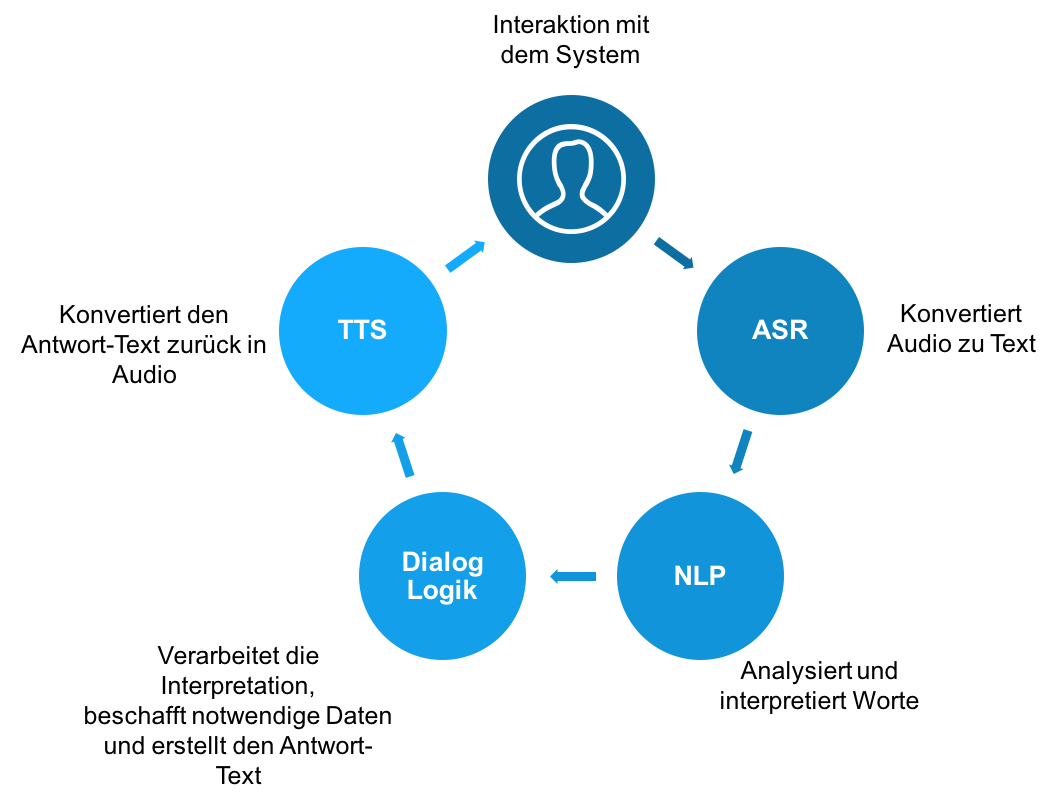
\includegraphics[width=\textwidth]{bilder/2_cuiFunktionsweise.png}
    \caption{Typische Komponenten und Funktionsweise eines VUI}
    \label{fig:cui-funktionsweise}
\end{figure}

Man kann diese \ac{VUI} Technologien an sich jedoch nicht als conversational bezeichnen. Dies soll anhand eines Beispiels von Amazon Alexa veranschaulicht werden, dass mit einer Konversation nicht viel zu tun hat.
 
\begin{center}
Nutzer: \textit{„Brauche ich heute in Nürnberg einen Regenschirm?“}\\
\textcolor{mybluelight}{Alexa: \textit{„In Nürnberg wird heute kein Regen erwartet.“}}\\
\end{center}

Alexa hat auch Anwendungsfälle, die mehr als eine einzelne Frage-Antwort-Interaktion erfordern. Den heutigen \acp{VUI} fehlt dennoch die Fähigkeit einen Schritt weiter zu gehen. Weg vom Kommandozeilen-Interface und hin zum \ac{CUI} \cite{pearl-design-vui}.

\begin{center}
\textit{„Many of today’s bots are kind of a hipster façade around the same basic command line interfaces consumers abandoned in the 1980s. They require specific syntaxes and understand only a limited vocabulary—but they sure have personality!“} \cite{hipster-facade-textio}
\end{center}

Konversation ist mehr als nur der Austausch von logischen Formulierungen. Verschiedene Handlungen wie zum Beispiel Fragen, Versprechungen und Komplimente finden statt \cite{mctear-cui}. Die Persönlichkeit der Konversationspartner hat einen großen Einfluss auf die Unterhaltung. Man stellt sich aufeinander ein und passt \ggf die Sprache an sein Gegenüber an. Ein weiterer Punkt ist der Kontext. Man kann sich im Verlauf einer Unterhaltung auf deren Vergangenheit beziehen. Im Folgenden ein Beispiel dazu. 

\begin{center} % so the minipage is centered
F: \textit{„Wer war Abraham Lincoln?“}\\
A: \textit{„Er war Präsident der Vereinigten Staaten.“}\\
F: \textit{„Wann hat er gelebt?“}\\
A: \textit{„Von 1809 bis 1865.“}\\    
\end{center}

Beim Stellen der zweiten Frage muss nicht explizit angegeben werden, wer gemeint ist. Dies wird aus dem Kontext heraus klar. Zusammengefasst lässt sich also sagen, dass folgende Kriterien ein typisches \ac{CUI} ausmachen: 
\begin{itemize}
    \item Ein Bewusstsein für den Kontext der Konversation
    
    \item Das Fehlen eines fixen Konversationsflusses und damit die Möglichkeit, den Kontext jederzeit zu wechseln
    
    \item Die Fähigkeit, den Benutzer nach kontextrelevanten Informationen zu fragen
    
    \item Persönlichkeit
\end{itemize}

Diese Art und Weise mit Schnittstellen zu kommunizieren bringt Vorteile mit sich. Wie in Kapitel \ref{sec:motivation} erwähnt, kann man einem \ac{CUI} die Frage stellen, anstatt sie über ein \ac{GUI} zu suchen. Das kommt auch Benutzern zu Gute, die mit der Bedienung grafischer Oberflächen Probleme haben. Es fällt ihnen möglicherweise leichter, ihr Vorhaben als Satz formuliert einzutippen \bzw in ein Gerät zu sprechen. Insbesondere \acp{VUI} eröffnen manch körperlich eingeschränkten Nutzern neue Wege der Interaktion mit Computern.\\
Das nächste Kapitel beschreibt das für die Arbeit verwendete System und geht auf dessen Funktionsweise ein. 

\section{Amazon Alexa Voice Service}
\label{sec:alexa-voice-service}
Amazon hat Alexa im November 2014 veröffentlicht. Wie bereits in Kapitel \ref{sec:conversational-user-interface} erwähnt, ist Alexa ein \ac{VUI} der neuen Generation. Es kann über die entsprechenden Endgeräte genutzt werden. Amazon hat zwei dieser Geräte zusammen mit Alexa veröffentlich. Die intelligenten Lautsprecher Echo \cite{amazon-echo} und Echo Dot \cite{amazon-echo-dot}, zu sehen in Abbildung \ref{fig:amazon-echos}. Mittlerweile sind weitere Ausführungen dazu gekommen. Für den weiteren Verlauf der Arbeit, wird als Vertreter aller Alexa Endgeräte ein Amazon Echo verwendet und schlicht als Echo, Alexa Endgerät oder Endgerät bezeichnet. Sämtliche Erläuterungen zur Funktionsweise und den Geräte-Merkmalen beziehen sich auf diesen.

\begin{figure}[h]
  \centering
  \begin{minipage}[b]{0.4\textwidth}
    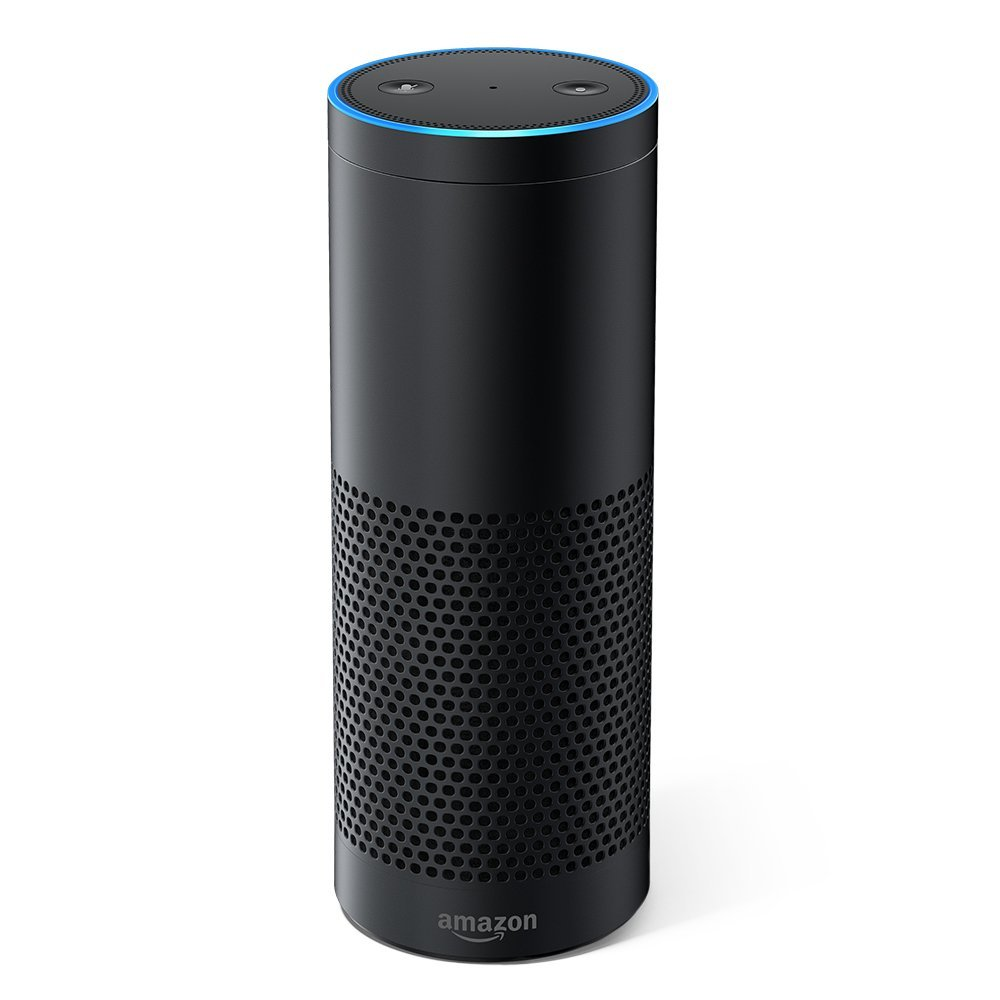
\includegraphics[width=\textwidth]{bilder/2_amazonEcho.jpg}
  \end{minipage}
  \begin{minipage}[b]{0.4\textwidth}
    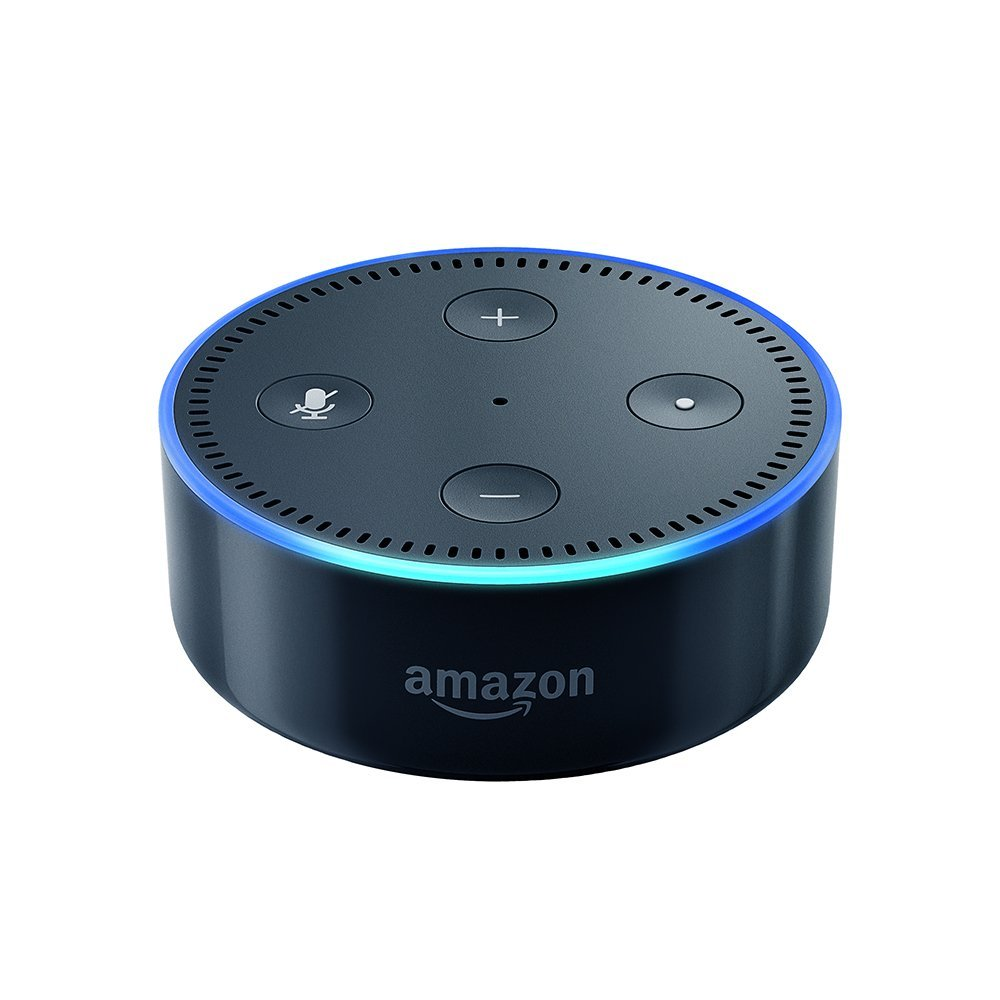
\includegraphics[width=\textwidth]{bilder/2_amazonEchoDot.jpg}
  \end{minipage}
  \caption{Amazon Echo und Echo Dot}
  \label{fig:amazon-echos}
\end{figure}

Die eigentliche Intelligenz steckt jedoch nicht im Echo. Alexa ist ein Cloud-Dienst \cite{amazon-developer-alexa}, der von Amazon über deren Server zur Verfügung gestellt und vom Endgerät genutzt wird (siehe Abbildung \ref{fig:alexa-komponenten}). 

\begin{figure}[!htb]
    \centering
    
\includegraphics[width=0.7\textwidth]{bilder/2_alexaDiagram.png}
    \caption{Alexa Endgerät zu Cloud-Dienst Verbindung}
    \label{fig:alexa-komponenten}
\end{figure}

Dabei bildet dieser Dienst einen Teil der \ac{VUI} Funktionalität ab und greift dabei auf die im Kapitel \ref{sec:conversational-user-interface} vorgestellten Technologien zurück. Um mit Alexa zu interagieren, muss ein Nutzer zunächst das sogenannte \textit{Wake Word} in den Echo sprechen. In der Grundeinstellung ist das Wort „Alexa“. Es kann jedoch auch auf „Echo“, „Amazon“ oder „Computer“ umgestellt werden. Mit einem Ton und dem leuchtenden Farbring auf der Oberseite des Echos signalisiert dieser, dass er sich mit dem Dienst verbunden hat und auf weitere Eingabe wartet. Nun kann man durch Sprache die gewünschten Funktionen nutzen. Der Lautsprecher kann sich nicht selbst aktivieren. Dies muss immer von einem Nutzer aus initiiert werden. \\
Alexa bringt bereits Basisfunktionalität mit, wie etwa Informationen zum Wetter, der Uhrzeit, das Verwalten von Timern und Listen und das Abspielen von Musik. Es ist jedoch auch möglich den Funktionsumfang durch zusätzliche Anwendungen, sogenannten Skills, zu erweitern. Um Skills zu nutzen die nicht in der Basisfunktionalität enthalten sind, muss man diese nach der Installation mit ihrem \textit{Invocation-Name} explizit ansprechen. In den meisten Fällen entspricht der Invocation-Name dem eigentlichen Namen des Skills. Es gibt zwei unterschiedliche Arten sie zu nutzen. Man kann sie öffnen und sich innerhalb der Anwendung bewegen, ohne den Namen wiederholen zu müssen. Die andere Möglichkeit ist das \textit{One-Shot-Model}. Hierüber wird der Skill beim Stellen der Frage direkt adressiert. Um beispielsweise die Anwendung „Abfallkalender“ \cite{abfallkalender} zu verwenden, welche Müllabfuhr Termine ausgeben kann, gibt es folgende Möglichkeiten. Öffnen des Skills: 

\begin{center} % so the minipage is centered
\textit{„Alexa, starte Abfallkalender“}\\
\textcolor{mybluelight}{Alexa: \textit{„Hallo hier ist der Abfallkalender, morgen am Montag wird Wertstofftonne abgeholt, kann ich sonst noch etwas für dich tun?}}
\end{center}
Nachdem der Abfallkalender geantwortet hat, kann man Fragen stellen wie: 

\begin{center} % so the minipage is centered
\textit{„Wann wird der Papiermüll abgeholt?“}\\
\textcolor{mybluelight}{Alexa: \textit{„Altpapier wird am Donnerstag dem 14. September abgeholt“}}
\end{center}

Das ergibt vor allem Sinn, wenn man mehrere Fragen an einen Skill hat. Über das One-Shot-Model kann man sich den Zwischenschritt sparen, wenn man nur eine einzige Information abrufen möchte.

\begin{center} % so the minipage is centered
Nutzer: \textit{„Alexa, frage Abfallkalender, wann der Papiermüll geholt wird?“}\\
\textcolor{mybluelight}{Alexa: \textit{„Altpapier wird am Donnerstag dem 14. September abgeholt“}}
\end{center}

Jeder mit einem Amazon Developer Account \cite{amazon-developer} kann Skills selbst entwickeln und Alexa Nutzern zur Verfügung stellen. Ein Skill besteht mindestens aus zwei Komponenten, dem \textit{Interaction Model} und dem \textit{Skill-Server}. 

\textbf{Interaction Model}\\
Man kann sagen, dass das Interaction Model aus \ac{VUI} Sicht das Frontend bildet. Hier gibt man Informationen wie den Namen des Skills, dessen Invocation-Name und die Adresse des Servers mit der Logik an (siehe Abschnitt Skill-Server). Obwohl beide meist identisch sind, dient der Name lediglich dessen Anzeige, während der Invocation-Name, die Worte für das Öffnen der Anwendung bestimmt. Des Weiteren wird im Interaction Model festgelegt, welche Formulierungen Alexa in Verbindung mit diesem Skill verstehen soll. Diese müssen in Form einer definierten Syntax angegeben werden. Die dabei verwendeten Begrifflichkeiten werden anhand eines Beispiels erklärt, wie man es bei der Verwendung des Wetter Skills finden kann.

\begin{center} % so the minipage is centered
\textit{„Alexa, \textcolor{mybluelight}{brauche ich \textcolor{red}{morgen} in \textcolor{red}{Nürnberg} einen Regenschirm?“}}
\end{center}

Da es sich bei dem Wetter Skill um eine Alexa Basisfunktionalität handelt, muss der Invocation-Name an dieser Stelle nicht genannt werden.\\

\textbf{\textit{Intent}}: Im Beispiel kann der Intent nicht direkt markiert werden. Er ergibt sich aus dem Verbund der Formulierung. Technisch gesehen ist es eine Funktion. Für den Wetter Skill könnte es beispielsweise einen Intent geben, der für alle Anfragen bezüglich des Niederschlags zuständig ist. Semantisch ist es die Essenz der Konversation oder auch die Absicht des Nutzers.\\

\textbf{\textit{Slot}}: Slots, im Beispiel \textcolor{red}{rot} markiert, sind eine Art Parameter. Unter Angabe von Slots haben Nutzer die Möglichkeit, ihre Anfragen zu parametrisieren \bzw zu spezifizieren. Im Beispiel sind \textit{\textcolor{red}{morgen}} und \textit{\textcolor{red}{Nürnberg}} Slots, die man durch andere Zeit- oder Ortsangaben ersetzen kann, \zB \textit{\textcolor{mybluelight}{„brauche ich am \textcolor{red}{10. Juni} in \textcolor{red}{New York} einen Regenschirm?“}}.\\

\textbf{\textit{Utterance}}: Eine Utterance, im Beispiel der Verbund aus blau und rot markiertem Text, ist eine Formulierung, die Slots enthalten kann. Über eine solche Formulierung wird ein Intent verwendet. Utterances werden explizit mit einem bestimmten Intent verknüpft. Ein Intent kann also von vielen Utterances angesprochen werden. Statt dem verwendeten Beispiel könnte man mit \textit{\textcolor{mybluelight}{„wird es \textcolor{red}{morgen} in \textcolor{red}{Nürnberg} regnen?“}} danach fragen.

\begin{figure}[!htb]
    \centering
    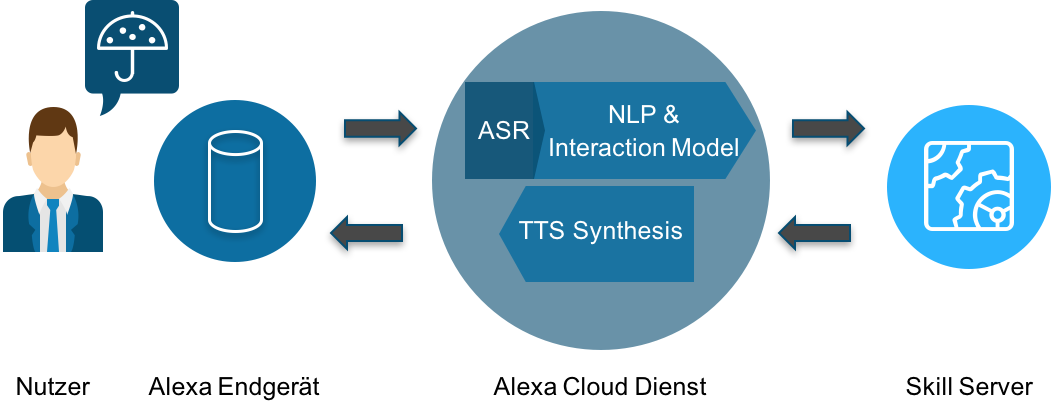
\includegraphics[width=0.7\textwidth]{bilder/2_alexaDiagramDetail.png}
    \caption{Alexa Komponenten und Funktionsweise}
    \label{fig:alexa-komponenten-funktionsweise}
\end{figure}

\textbf{Skill-Server}\\
Betrachtet man das Interaction Model als \ac{VUI}-Frontend, bildet der Skill-Server das Backend ab. Alexa sendet interpretierte Daten einer Spracheingabe über die im Model hinterlegte Adresse an die \textit{\ac{REST}}-Schnittstelle des Skill-Servers. Hier werden diese verarbeitet und  gegebenenfalls reale Daten entsprechend des Nutzungskontextes bereitgestellt. Die Antwort, die der Echo ausgeben soll, wird hier in Textform erstellt und an Alexa zurückgesandt. Das \ac{TTS} System aus Abbildung \ref{fig:alexa-komponenten-funktionsweise} konvertiert diesen Text in Audio. Im Anschluss wird das Audio an den Echo gesendet und von diesem ausgegeben. Es ist auch möglich grafische Elemente in die Interaktion einzubinden. Über sogenannte \textit{Skill Cards} kann man fest definierte, nicht veränderbare Strukturvorlagen mit statischem Text und Bildern erstellen. Diese kann der Benutzer über die Alexa Smartphone App auf seinem mobilen Gerät empfangen und einsehen. Da diese Vorlagen keine dynamischen Inhalte erlauben sind Anwendungsfälle, die auf komplexe, visuelle Elemente zurückgreifen müssen, wenig zweckdienlich. Beispiele hierfür sind detailreiche Statistiken, lange Listen und die Planung von Routen.

\section{Bankkonten-Management}
\label{sec:bankkonten-management}
Laut Statistiken aus dem Jahr 2017 (siehe \cite{online-bank-statista} \cite{online-bank-heise} \cite{online-bank-destatis}) verwendet in etwa jeder zweite in Deutschland Online-Banking. Das heißt sie erledigen ihre Bankgeschäfte bequem vom Rechner oder anderen Endgeräten aus. Kreditinstitute und Banken stellen hierfür ihren Kunden kostenlose Online-Portale und Anwendungen für mobile Endgeräte zur Verfügung. Mit Bankkonten-Management sind in dieser Arbeit einerseits Funktionen gemeint, die man überwiegend aus diesen Anwendungen kennt. Dazu zählen \ua die Anzeige des Kontostandes, das Durchführen von Überweisungen und die Einsicht der Umsätze. Darüber hinaus gibt es weitere Dienste, die mittlerweile auch von vielen Banken angeboten werden, jedoch meist aus modernen Finanzmanagement-Anwendungen von Drittanbietern bekannt sind. Beispiele hierfür ist der \textit{Finanzmanager} der Volksbanken Raiffeisenbanken \cite{vrbank-finanzmanager}, welcher auf Wunsch in das Online-Banking-Portal integriert werden kann oder die Smartphone-Applikation \textit{fymio} der TeamBank AG \cite{fymio}. Da Teile dieser Funktionalität und deren Begrifflichkeiten in Überlegungen und der Konzeption im weiteren Verlauf der Arbeit einfließen, werden diese kurz erläutert. Für die Arbeit werden sie in der hier beschriebenen Art und Weise verwendet und können von den Definitionen in den genannten Anwendungen Finanzmanager und fymio abweichen.

\textbf{\textit{Finanzperiode}}: Eine Finanzperiode beginnt mit dem Gehaltseingang und endet vor dem nächsten. \\
\textbf{\textit{Budget}}: Mit Budget ist in dieser Arbeit das bis zum Ende der Finanzperiode verfügbare Guthaben gemeint, dass sich aus Einnahmen und Fixkosten errechnet.\\
\textbf{\textit{Multibanking}}: Mit Multibanking ist die Möglichkeit gemeint, mehrere Konten verschiedener Banken und Kreditinstitute parallel an eine zentrale Anwendung anzubinden.\\
\textbf{\textit{Hauptkonto}}: Damit ist das Konto gemeint, auf das sämtliche Berechnungen und Aktionen angewandt werden. Auch wenn es möglich ist mehrere Konten anzubinden (\vgl Multibanking), muss eines davon als Hauptkonto selektiert werden. Möchte man beispielsweise vor der Durchführung einer Überweisung das Budget ausgeben lassen, wäre es irreführend, dies von allen Konten zusammen zu rechnen.\\
\textbf{\textit{Sparziel}}: Mit Sparzielen können Nutzer auf einem Sparkonto für einen beliebigen Zweck sparen. Dabei kann man je nach Wunsch einmalige oder regelmäßige Zahlungen an dieses Ziel übertragen. Als Teil des Sparkontos, existiert ein solches Ziel nur virtuell und nicht als eine Art separates Unterkonto.
\chapter{Konzeption}
\label{cha:konzeption}
In diesem Kapitel werden die Anforderungen an das \ac{CUI}  und ein Konzept für die Implementierung erarbeitet. Dafür werden Ansichten und Methoden aus dem Bereich des Usability Engineering verwendet. Usability \bzw \textit{Gebrauchstauglichkeit} definiert sich wie folgt:

\begin{quote}
    Das Ausmaß, in dem ein Produkt durch bestimmte Benutzer in einem bestimmten Nutzungskontext dazu genutzt werden kann, bestimmte Ziele effektiv, effizient und zufriedenstellend zu erreichen \cite{richter-ux-compact}.
\end{quote}

\textit{Effektivität} misst dabei die Genauigkeit und Vollständigkeit in dem das Ziel des Benutzers erreicht wird. \textit{Effizienz} misst das Verhältnis von Aufwand zu erreichter Effektivität bei der Zielerreichung. \textit{Zufriedenstellung} gibt Aufschluss über die Freiheit von Beeinträchtigung und positive Einstellung des Benutzers gegenüber der Nutzung des Produktes. Letzteres ist schwieriger zu messen, da dieses Kriterium zu einem großen Teil die subjektive Meinung der Benutzer widerspiegelt. Der \textit{Nutzungskontext} umfasst die Benutzer, deren Ziele und Aufgaben, sowie die physische und soziale Umgebung, in der das Softwaresystem genutzt wird \cite{richter-ux-compact}. Die Benutzergruppe lässt sich im Fall des Bankkonten-Managements schlecht eingrenzen und schließt somit jeden ein, der ein Bankkonto besitzt und seine Bankgeschäfte online erledigt.\\
Die Usability eines Produktes ist ein nicht zu unterschätzender Faktor in der Softwareentwicklung. Das Anwenden dieses Paradigma liefert wichtige Erkenntnisse, die in den Entwicklungsprozess einfließen. Noch bedeutsamer als bei der Entwicklung von grafischen Schnittstellen ist die Anwendung dieser Methodiken im Bereich der CUIs. Gerade weil Benutzer auf natürliche Art und Weise mit dem System interagieren, müssen sie während des gesamten Entwicklungsprozesses im Fokus stehen. Jeder Mensch denkt, spricht und formuliert anders. Dabei sind nicht nur die Formen der Eingabe zu untersuchen, essenziell für die Usability ist auch die Ausgabe. \ac{VUI}- \bzw \ac{CUI}-Endgeräte, wie auch in diesem Fall der Echo, haben oft nur eingeschränkte oder gar keine grafische Unterstüzung. Es gibt also keine visuellen Anker, die dem Benutzer bei der Navigation helfen. Die auditiven Antworten des Systems müssen Aufschluss darüber geben, was gerade passiert und in welchem Zustand es sich befindet.\\ 
Ein weiterer wichtiger Aspekt ist die Persönlichkeit. Als ein Faktor der bei \acp{CUI} eine Rolle spielt, muss man damit vorsichtig sein. Es ist zu untersuchen, welche Charakteristiken Benutzer bei der Verwendung  womöglich als störend oder unnatürlich empfinden. Des Weiteren ist darauf zu achten, die Persönlichkeit des \acp{CUI} nicht zu menschlich wirken zu lassen. Masahiro Mori, ein japanischer Robotiker hat 1970 das \textit{uncanny valley} beschrieben, zu sehen in Abbildung \ref{fig:uncanny-valley} \cite{watson-uncanney-valley}. 

\begin{figure}[!htb]
    \centering
    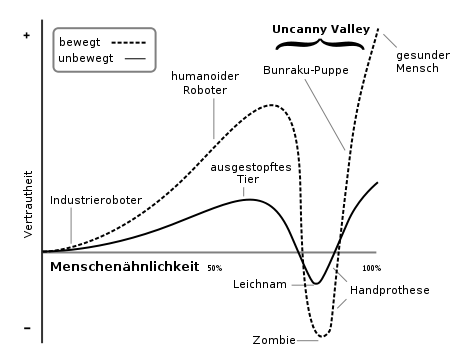
\includegraphics[width=1.0\textwidth]{bilder/3_uncannyValley.png}
    \caption{Das Phänomen des unheimlichen Tals -  „uncanny valley“}
    \label{fig:uncanny-valley}
\end{figure}

Es wird verwendet um zu zeigen, dass die Akzeptanz gegenüber technisch simuliertem Verhalten vom Realitätsgehalt abhängt. Dabei verzeichnet eine Annäherung an das menschenähnliche Verhalten innerhalb eines bestimmten Bereiches einen signifikanten Einbruch dieser Akzeptanz.

\section{Requirements Engineering}
\label{sec:requirements-engineering}
In diesem Kapitel wird die Anforderungsanalyse unter Berücksichtigung der genannten Aspekte beschrieben. Dieser Schritt ist äußerst wichtig, um das System auf die im Fokus liegende Zielgruppe abzustimmen. Die Methoden, der Grund ihrer Anwendung und die Ergebnisse sind in den jeweiligen Unterkapiteln näher erklärt.

\subsection{Umfrage}
\label{subsec:online-umfrage}
Um sich einen groben Überblick zu verschaffen soll zunächst geklärt werden warum und in welchem Umfang Online-Banking verwendet wird. Um das Ergebnis aufgrund einer möglichen Voreingenommenheit gegenüber \acp{VUI} nicht zu verfälschen, soll dafür der Zusammenhang mit diesen unerwähnt bleiben. Wie bereits festgestellt, besteht die Zielgruppe aus Personen, die ihre Bankgeschäfte über Online-Banking abwickeln. Dennoch wäre es sehr interessant festzustellen was die Gründe für diejenigen sind, die Online-Banking nicht nutzen.\\
Um ein breiteres Spektrum an Information zu erhalten, werden hierfür quantitative Daten über eine anonyme Online Umfrage gesammelt. Diese sollen auch helfen die Intention der Benutzer bei der Ausführung bestimmter Funktionen zu ergründen. Für die Durchführung der Umfrage stehen die folgenden drei Anwendungen in der engeren Auswahl. 

\begin{itemize}
    \item Google Forms \cite{google-forms}
    \item Survey Monkey \cite{survey-monkey}
    \item Umfrage Online \cite{umfrage-online}
\end{itemize}

Tabelle \ref{tab:umfrage-toolauswahl} stellt den Funktionsumfang der Anwendungen mit den Anforderungen an diesen gegenüber.

\begin{table}[!htb]
\centering
 \begin{tabular}{ | m{5cm} || C{2cm}| C{2cm} | C{2cm} |} 
 \hline
 Anforderungen & Google Forms & Survey Monkey & Umfrage Online
 \\
 \hhline{=::===}
 16 Fragen & \cmark & \danger & \cmark\\ 
 \hline Umfragelogik & \xmark & \danger & \cmark\\
 \hline Auswertung & \cmark & \cmark & \cmark\\
 \hline Anonymisierung & \cmark & \cmark & \cmark\\ 
 \hline Mehrfache Teilnahme unterbinden & \danger & \cmark & \cmark\\ 
 \hline
\end{tabular}
\caption{Auswahlhilfe für die Anwendung zur Durchführung der Umfrage}
\label{tab:umfrage-toolauswahl}
\end{table}

Die Anforderungen resultieren \ua aus dem erstellten Fragebogen, welcher zusammen mit den Antworten aus Gründen der besseren Lesbarkeit und des Leseflusses im \nameref{sec:Anhang} unter Kapitel \ref{sec:ausfuehrung-online-umfrage} zu finden ist. Erfüllte Anforderungen sind in Tabelle \ref{tab:umfrage-toolauswahl} mit grünen Haken, nicht erfüllte mit einem roten „X“, versehen. Die Warndreiecke sagen aus, dass diese Anforderungen nur unter bestimmten Bedingungen erfüllt werden. Im Fall von Survey Monkey können diese nur mit zusätzlichem Kostenaufwand erfüllt werden. Google Forms wiederum verlangt für das Unterbinden mehrfacher Teilnahmen pro Befragten, dass sich diese registrieren.\\
Wegen den aus Tabelle \ref{tab:umfrage-toolauswahl} ersichtlichen Gründen, fällt die Wahl auf die Anwendung Umfrage Online. Es erfüllt alle Voraussetzungen und kann außerdem ohne zusätzliche Kosten genutzt werden. Im Anschluss werden die wichtigsten Ergebnisse und Erkenntnisse zusammengefasst.\\
Der Prozentsatz der Online-Banking-Nutzer in der Umfrage unterscheidet sich deutlich von den in Kapitel \ref{sec:bankkonten-management} referenzierten Statistiken. Über 90 Prozent der Umfrage-Teilnehmer nutzen Online-Banking. Dies ist möglicherweise auf das Durchschnittsalter zurückzuführen. Wie aus Frage 16 ersichtlich ist, sind über 46 Prozent der Teilnehmer zwischen 18 und 30 Jahre alt. Nur knapp 12 Prozent sind älter als 50. Die Diskrepanz lässt sich also dadurch erklären, dass Personen im hohen Alter weniger geneigt sind ihre Bankgeschäfte online zu erledigen. Weiterhin kann die Umfrage nur von Personen mit einem Computer oder mobilen Endgerät durchgeführt werden. Dies kann ein weiterer Grund dafür sein.\\
Als Hauptgründe für die Nutzung von Online-Banking sind vor allem der schnelle Zugriff und die Bequemlichkeit bei der Verwendung genannt. An diesen zwei Kriterien kann man mit einem \ac{CUI} sehr gut ansetzen. Genau das sind mitunter große Vorteile dieser Systeme und Gründe für deren Einsatz.\\
Weiterhin werden die Intentionen der Nutzer beim Prüfen ihres Kontostandes \bzw ihrer Umsätze erfragt. Die am häufigsten genannten Intentionen sind Kontrolle und Überwachung des Guthabens. Dennoch gibt es sehr interessante Antworten, die man als Grundlage für weitere Anwendungsfälle nutzen kann. Darunter zu finden sind sinngemäß:

\begin{itemize}
    \item\textit{„Was kann ich mir noch leisten?“}
    \item\textit{„Gibt es Auffälligkeiten?“}
    \item\textit{„Ist mein Lohn/Gehalt schon da?“}
    \item\textit{„Habe ich Geld aus Gutschriften erhalten?“}
    \item\textit{„Ich möchte eine einfache Übersicht“}
\end{itemize}

Da viele Online-Banking-Plattformen auch den Handel mit Aktien \bzw das Verwalten eines Wertpapier Depots ermöglichen, sind auch diesbezüglich Fragen in die Umfrage eingeflossen. Anwendungsfälle aus dem Aktienbereich sind denkbare und sinnvolle Erweiterungsmöglichkeiten für ein Banking-\ac{CUI}. Da der Fokus der Arbeit auf dem Management von Bankkonten liegt werden diese Fälle nicht weiter ausgebaut, sondern nur als eine Möglichkeit zur Erweiterung gesehen.\\
Die Sicherheitsbedenken bei der Nutzung von Online-Banking sind sehr hoch. Knapp 80 Prozent der Befragten haben solche Bedenken. Gerade das ist auch bei der Entwicklung des \ac{CUI} ein sehr wichtiger Punkt, der im weiteren Verlauf der Arbeit aufgegriffen wird.\\
Des Weiteren wird nach Vorschlägen gefragt, wie die Verwendung der Online-Banking-Anwendungen effizienter laufen könnte. Unter den Antworten befinden sich sinngemäß auch Folgende:

\begin{itemize}
    \item\textit{„Mehrere Unterkonten in einem Konto, um Geld auf verschiedene Themen aufzuteilen“}
    \item\textit{„Bei Smartphone App Fingerabdruck statt Passwort bei Login“}
    \item\textit{„Sicherheit und Handling verbessern“}
    \item\textit{„Zugriff auf alle Sparbücher und Konten“}
    \item\textit{„Überweisungen über Handy App mit digitalem Überweisungsformular, dass man nur noch bestätigen muss“}
\end{itemize}

Unterkonten können mit den in Kapitel \ref{sec:bankkonten-management} erwähnten Sparzielen verglichen werden. Ebenso stimmt der Punkt Zugriff auf alle Sparbücher und Konten mit dem Begriff des Multibankings aus dem gleichen Kapitel überein.\\
Die hier erlangten Intentionen und Erkenntnisse werden im weiteren Verlauf der Arbeit aufgegriffen, genauer betrachtet und entwickelt.

\subsection{Interviews}
\label{subsec:interviews}
Durch die Erhebung der quantitativen Daten in Kapitel \ref{subsec:online-umfrage} wird ein allgemeiner Einblick in das Nutzungsverhalten beim Online-Banking gewährt. Für einen tieferen Einblick  sollen nun qualitative Daten gesammelt werden. Es soll auch konkret auf \acp{VUI} eingegangen werden. Dabei sind die Meinung und Akzeptanz von potentiellen Nutzern gegenüber dieser Systeme in Erfahrung zu bringen. Des Weiteren wäre es interessant zu sehen, wie Befragte auf die Kombination von Online-Banking und Sprachassistenzsystemen reagieren. Hier bietet die Methode des Interviews klare Vorteile. Es ist möglich auf die Antworten des Gegenübers einzugehen und im Fall von Unklarheiten nachzufragen. Wird das Interview von Angesicht zu Angesicht durchgeführt, können zusätzlich die Mimik und Gestik des Befragten Erkenntnisse liefern.\\
Aus den Kapiteln \ref{sec:conversational-user-interface} und \ref{sec:alexa-voice-service} ist bekannt, dass man einem \ac{CUI} Formulierungen vorgeben muss, damit es diese versteht. Ein Interview bietet auch eine gute Möglichkeit, nach solchen Formulierungen zu fragen.\\
Das Interview wird über einen Audiorekorder aufgezeichnet. Damit ist sichergestellt, dass Informationen nicht verloren gehen und eine Auswertung in schriftlicher Form nachträglich erfolgen kann. Dadurch ist der Interviewer in der Lage, parallel Notizen anzufertigen. Um die Anonymität der Befragten zu gewährleisten wird lediglich die schriftliche Ausarbeitung dokumentiert. Eine entsprechende Einverständniserklärung wird jedem Teilnehmer vor Durchführung des Interviews vorgelegt. Die Erklärung ist im \nameref{sec:Anhang} unter Kapitel \ref{sec:ausfuehrung-interview-einverstaendnis} zu finden, der Fragebogen selbst unter Kapitel \ref{sec:ausfuehrung-interview-fragebogen}. Wichtig bei der Durchführung eines Interviews sind die folgenden Verhaltensregeln: 

\begin{itemize}
    \item Einen neutralen und vertrauenswürdigen Eindruck vermitteln
    \item Jeden Befragten respektvoll behandeln
    \item Es gibt keine falschen Antworten
    \item Den Befragten nicht widersprechen
    \item Bei Unklarheiten nachfragen
\end{itemize}

Deren Einhaltung stellt sicher, dass die Gedanken und Meinungen des Nutzers erfasst und verstanden werden können. Es ist nicht zielführend dem Gegenüber die eigene Meinung näher zu bringen. Eine solche Beeinflussung verfälscht lediglich die Ergebnisse.\\ 
Vier Personen haben an den Interviews teilgenommen. Die schriftliche Auswertung ist im \nameref{sec:Anhang} unter Kapitel \ref{sec:ausfuehrung-interview-auswertung} dokumentiert. Diese liegt in einer sinngemäßen, stichpunktartigen Zusammenfassung vor. Die Reihenfolge der jeweiligen Antworten ist willkürlich gewählt und entspricht nicht der chronologischen Anordnung der Interviews. Für einen besseren Überblick werden die wichtigsten Ergebnisse hier zusammengefasst. Im Anschluss wird die Durchführung an sich rekapituliert.\\
Die Altersgruppe der Befragten liegt zwischen 22 und 26. Im Allgemeinen ist die Meinung der Befragten gegenüber \acp{VUI} eher skeptisch, befremdlich und mit großen Bedenken verbunden. Dennoch wird die Technologie durchaus als praktisch, zeitsparend und interessant erkannt. Die Erfahrung der Teilnehmer mit Sprachassistenten ist eher gering. Die Verteilung der Online-Banking-Nutzung spiegelt in etwa den Trend der Online Umfrage wider. Die Intentionen bei der Nutzung und auch die Sicherheitsbedenken unterscheiden sich nicht zu den Erkenntnissen aus der Umfrage. Gerade weil es um die Verbindung einer neuen Technologie mit einem ohnehin sicherheitskritischen Bereich wie Finanzen geht, ist die Skepsis groß. Die Teilnehmer geben an ihre Bankgeschäfte überwiegend alleine und in einem diskreten Umfeld durchzuführen. Durch das Erfragen von spezifischen Formulierungen zu Anwendungsfällen, können nur vereinzelte Ergebnisse erzielt werden. Die Bereitschaft zur Nutzung eines solchen Systems ist eher gering und mit Kriterien, wie \zB guten Bewertungen anderer Benutzer, verbunden.\\ 
Zusätzlich sind die folgenden Anmerkungen der Teilnehmer dazu gekommen:

\begin{itemize}
    \item Die Bereitstellung von Informationen bezüglich Datenschutz und verwendeter Sicherheitsstandards des Systems sind wünschenswert. Dies trägt maßgeblich zur Entscheidung für oder gegen die Nutzung bei
    
    \item Wegen des schnellen Zugriffs, ist eine Funktion für eine ebenso schnelle Kontoübersicht nützlich
    
    \item Bei Überweisungen soll das Verstandene noch einmal ausgegeben und vom Nutzer bestätigt werden, bevor die Überweisung durchgeführt wird
    
    \item Wird das Konto mit der getätigten Überweisung überzogen, soll das System den Nutzer vorher warnen
    
    \item Der Benutzer soll im Falle einer Buchung benachrichtigt werden
    
    \item Die Verwaltung von Finanzen ist ein seriöses Thema. Das System sollte den Benutzer nicht duzen.
\end{itemize}

Auch wenn die Erkenntnisse aus den konkreten Interview Fragen wenig überraschend sind, können dennoch wichtige Gesichtspunkte in die Entwicklung des Systems einfließen. Vor allem die zusätzlichen Vorschläge und Ideen der Befragten erscheinen äußerst sinnvoll und finden im weiteren Verlauf der Arbeit Verwendung.\\
Trotzdem gibt es auch etwas zu beanstanden. Das Alter der Befragten entspricht bei weitem nicht der kompletten Zielgruppe. Fragen nach Sprachbefehlen für konkrete Anwendungsfälle haben den Fluss der Konversation negativ beeinträchtigt. Daraus entstandene Verzögerungen haben zu sichtlich unangenehmenen Situationen geführt. Aufgrund dessen wurden Fragen übersprungen. Die Folge sind die wenigen Ergebnisse aus diesem Teil der Interviews. 

\subsection{Personas}
\label{subsec:personas}
Die Methode der Personas ist ein Instrument, um die unterschiedlichen Bedürfnisse der Benutzer zu modellieren und daraus passende Lösungen abzuleiten. Sie stellen prototypische Benutzer dar und verkörpern ihre unterschiedlichen Ziele, Verhaltensweisen und Eigenschaften, die im Hinblick auf das zu entwickelnde Produkt relevant sind \cite{richter-ux-compact}. Die Basis für deren Modellierung bilden die gesammelten Daten aus den vorangegangenen Kapiteln \ref{subsec:online-umfrage} und \ref{subsec:interviews}.\\
Personas sollen einfach verinnerlicht werden. Dazu kann man ihnen durchaus Namen, Bild, Alter und Charakterzüge zuweisen \cite{richter-ux-compact}. Aus Gründen der Lesbarkeit wird im Folgenden nur eine der Personas abgebildet. Zu den anderen wird lediglich eine Zusammenfassung gegeben. Die Abbildungen aller Personas sind im \nameref{sec:Anhang} unter Kapitel \ref{sec:anhang-personas} zu finden.\\\\
Abbildung \ref{fig:alena-meier} zeigt die Persona Alena Meier. Sie ist eine organisierte Frau, die parallel viele Konten zu verwalten hat. Um ihr einen schnellen Überblick zu gewährleisten, ist es wichtig die benötigten Informationen des jeweiligen Kontos gebündelt abrufbar zu machen. Gleichzeitig muss sie die Zahlungen ihrer Mieter im Auge behalten. Um das zu schaffen ist sie auf Technik angewiesen. Da ihr mit der Arbeit und ihren Finanzgeschäften nicht viel Zeit übrig bleibt, vergeudet sie diese nur ungern an unausgereifte Technik.

\begin{figure}[!htb]
    \centering
    \fbox{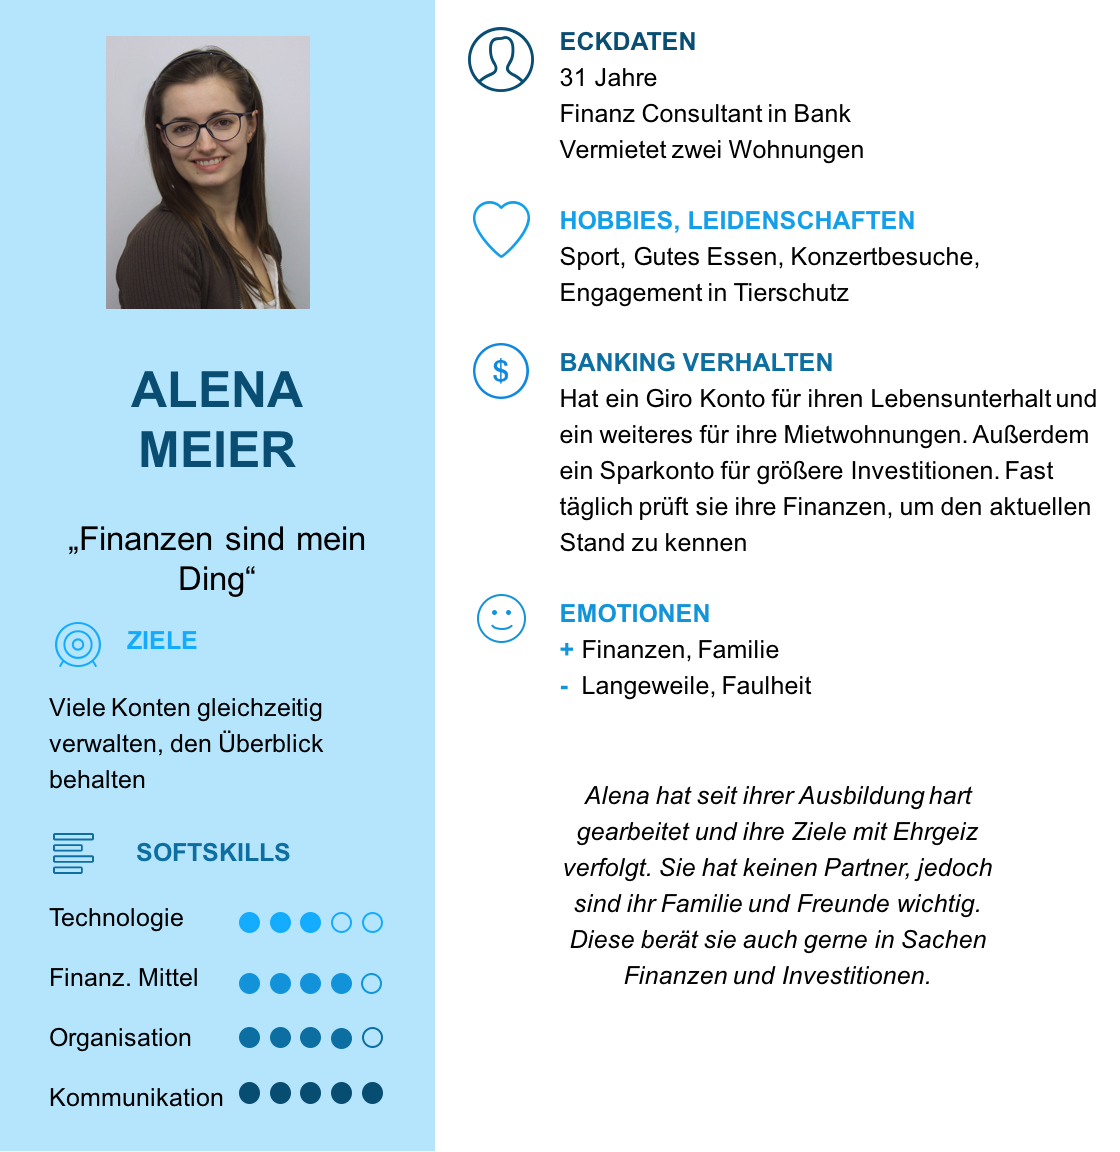
\includegraphics[width=1.0\textwidth]{bilder/3_alenaMeier.png}}
    \caption{Persona Alena Meier}
    \label{fig:alena-meier}
\end{figure}

Josef Lech aus Abbildung \ref{fig:robert-trier} kann durch seine körperliche Einschränkung nicht mehr den gewohnten Weg zur Bank nehmen. Er kommt nur schwer mit neuer Technik zurecht. Die Verwendung einer Online-Banking-Plattform ist ihm zu kompliziert. Ein \ac{VUI} kann hier einen guten Ansatz bilden. Über natürliche Sprache fällt es dem Rentner eventuell einfacher, seine Bankgeschäfte zu erledigen. Die Ausgaben des Banking Skills müssen aussagekräftig und hilfreich sein, damit dieser für Josef nutzbar wird.\\\\
Abbildung \ref{fig:robert-trier} zeigt die Persona Robert Trier, der großes Interesse daran hat neue Technologien zu verwenden. Als Fachmann weiß er aber auch, dass Datenschutz und Sicherheit äußerst wichtig sind. Bevor er neue Technik nutzt, erkundigt er sich über verwendete Sicherheitsstandards. Unbefugten darf es nicht möglich sein sensible Daten zu entwenden.\\\\
Die Persona Daniela Friedmann aus Abbildung \ref{fig:daniela-friedmann} muss ihr Konto ständig im Blick haben, damit sie es beim Ausgehen mit Freunden nicht überzieht. Dennoch möchte sie nicht jeden Tag daran erinnert werden, dass sie wenig Geld hat. Wegen der hin und wieder vorkommenden Indiskretion ihrer WG Mitbewohner, sind auditive Ausgaben von sensiblen Daten eher schwierig. Es muss eine Möglichkeit geben das zu umgehen. Außerdem muss im Falle ihrer Abwesenheit gewährleistet sein, dass kein anderer Zugriff auf ihre Daten erhält.\\\\
Das Modellieren der Personas liefert wichtige Erkenntnisse. Nicht nur Bedürfnisse und Ziele der einzelnen Personas können das Konzept bereichern. Auch der Nutzungskontext kann besser verstanden werden. Situationen, in denen das Produkt verwendet wird werden sichtbar. Darunter auch solche, die die Nutzung einschränken oder auch unmöglich machen. Das folgende Kapitel \ref{subsec:user-stories} beschreibt die Entwicklung der \textit{User Stories}, die aus den empirischen Daten und dem aktuellen Verständnis für die Zielgruppe resultieren.

\subsection{User Stories}
\label{subsec:user-stories}
Vor dem Einsatz eines \ac{CUI} ist immer zu evaluieren, welchen Mehrwert man mit dessen Einsatz für potentielle Benutzer generiert. Daher stellt sich in diesem Fall nicht die Frage, ob ein \ac{CUI} eine grafische Online-Banking-Anwendung ablösen kann. Es ist vielmehr als eine Ergänzung zu sehen. Eine, die für bestimmte Anwendungsfälle Vorteile bietet. Es gilt genau zu überlegen welche Funktionen hier sinnvoll sind und welche nicht.\\
Dieses Kapitel beschreibt den Funktionsumfang des Banking-Skills in Form von \textit{User Stories}. Sie basieren auf den Ergebnissen der vergangenen Kapitel \ref{subsec:online-umfrage} bis \ref{subsec:personas}. Wie ein \textit{Use Case} beschreibt auch die \textit{User Story} eine Funktion aus Sicht des Nutzers. Der Unterschied liegt in der Granularität. Use Cases beschreiben den Vorgang feingranularer. Aus User Stories wird jedoch die Intention der Benutzer direkt erkenntlich, was hier auch der Grund für deren Verwendung ist.\\
Aus Übersichtszwecken und da sich die User Stories im weiteren Verlauf der Arbeit ändern können, ist eine komplette Liste im \nameref{sec:Anhang} unter Kapitel \ref{sec:anhang-user-stories} zu finden. Hier wird lediglich ein Überblick über die Kernfunktionen des Systems gegeben.

\begin{itemize}
    \item\textbf{Hilfe Funktion}: Die Hilfe kann einem Benutzer vermitteln, welche Funktionen verwendet werden können und über welche Formulierungen er diese aufrufen kann. Denkbar ist hier auch eine kontextbezogene Hilfe. Das soll vor allem den Benutzern helfen, die \acp{VUI} \bzw den Skill zum ersten Mal verwenden. Auch Nutzer, die ihn nur selten verwenden können davon profitieren.
    
    \item\textbf{Profile verwalten/Authentifizierung}: Da jeder Benutzer mit den eigenen Bankkonten und Daten arbeitet, ist ein Authentifizierungsmechanismus unabdingbar. Nutzern muss es möglich sein sich zu registrieren und das angelegte Profil zu verwalten.
    
    \item\textbf{Bankkonten verknüpfen}: Damit Nutzer ihre Bankkonten verwalten können, müssen diese zunächst an das System angebunden werden.
    
    \item\textbf{Hauptkonto wählen}: Aus den in Kapitel \ref{sec:bankkonten-management} genannten Gründen müssen Nutzer in der Lage sein, eines der verknüpften Konten als Hauptkonto zu setzen. 
    
    \item\textbf{Vorlagen verwalten}: Damit Überweisungen schnell und einfach über Spracheingaben durchgeführt werden können soll es möglich sein, Zielkonten als Vorlagen zu speichern. Nutzern ist es möglich diesen Vorlagen Namen zuzuweisen, um diese zu adressieren. 
    
    \item\textbf{Kontostand}: Benutzern soll es möglich sein, den aktuellen Kontostand abzurufen.
    
    \item\textbf{Transaktion}: Unter Verwendung einer Vorlage und eines Geldbetrages können Benutzer Überweisungen durchführen, wie zum Beispiel „Überweise \textit{50} Euro an \textit{Julian}“. Das Verstandene muss vom System wiederholt und vom Benutzer bestätigt werden, bevor die Überweisung durchgeführt wird. Des Weiteren muss eine Möglichkeit zur \textit{\ac{TAN}} Eingabe geschaffen werden, um die Transaktion zu authentifizieren. Das Ausfüllen von Überweisungsträgern unter Angabe des \textit{\ac{IBAN}} soll nicht möglich sein. Die Eingabe langer Buchstaben und Ziffer Kombinationen über Sprache kann vor allem bei Eingabefehlern schnell frustrieren. Dafür können Benutzer auf eine Online-Banking-Plattform \bzw Überweisungsträger aus Papier zurückgreifen. Das ist ein gutes Beispiel für die Koexistenz eines \ac{CUI} mit bestehenden \acp{GUI}.
    
    \item\textbf{Gehaltseingang prüfen}: Als eine der Intentionen aus der \nameref{subsec:online-umfrage}, sollen Nutzer prüfen können, ob ihr Gehalt für die aktuelle Finanzperiode bereits eingegangen ist. Ein Vorteil dieser Ausgabe ist, dass es sich dabei nicht um sensible Daten handelt. Die Beantwortung soll lediglich eine Art „ja“ oder „nein“ beinhalten. Die Höhe des Gehaltes wird dabei nicht genannt. 
    
    \item\textbf{Budget abrufen}: Teilnehmer der \nameref{subsec:online-umfrage} aus Kapitel \ref{subsec:online-umfrage} und der \nameref{subsec:interviews} aus Kapitel \ref{subsec:interviews} geben an, dass ein schneller Überblick über das Konto wünschenswert ist. Das Budget verrät, wie viel am Ende der aktuellen Finanzperiode auf dem Konto bleibt. Dies wird anhand des bisherigen Ausgabeverhaltens ermittelt. Benutzer sind dadurch in der Lage, ihr Verhalten gegebenenfalls anzupassen.
    
    \item\textbf{Fixkosten}: Abfragen zu Fixkosten komplettieren die Funktion des schnellen Überblicks und erlauben den Benutzern zu prüfen, wie viel Geld sie regelmäßig ausgeben. Beispiele hierfür sind „Miete“, „Strom-“ und „Heizkosten“.
    
    \item\textbf{Umsatzdaten}: Natürlich macht es wenig Sinn sämtliche Umsätze mehrerer Tage auszugeben. Das ist ein typisches Beispiel für einen schlechten \ac{CUI} Anwendungsfall. Lange, komplexe Listen können von einer grafischen Oberfläche wesentlich verständlicher und eleganter dargestellt werden. Dennoch können Nutzer durch gezielte Fragen schnell an Informationen kommen. Denkbar sind Abfragen zu bestimmten Zahlungsempfängern \bzw -sendern, Beträgen oder Verwendungszwecken. 
    
    \item\textbf{Sparziele verwalten}: Benutzern soll es möglich sein Sparziele zu verwalten. Damit können für bestimmte Themen Geld gespart werden.
\end{itemize}

Die hier beschriebenen Funktionalitäten spiegeln die Erkenntnisse aus den vorangegangenen Kapiteln wider. Dennoch ist sicherzustellen, dass die Daten auch richtig interpretiert werden. Zu diesem Zweck werden im Folgenden Nutzungsszenarien erstellt. Auf Basis dieser Szenarien werden in Kapitel \ref{sec:prototyping} User Tests durchgeführt, um die bisherigen Ergebnisse zu evaluieren.

\subsection{Szenarien}
\label{subsec:szenarien}
Anwendungsszenarien sind ein zentrales Element in der nutzerorientierten Entwicklung. Sie schlagen die Brücke zwischen den Anforderungen und dem Entwurf eines neuen Konzeptes. Szenarien beschreiben anhand realistischer Beispiele wie Benutzer mit dem zu entwickelnden Produkt interagieren \cite{richter-ux-compact}. Die in Kapitel \ref{subsec:user-stories} erschlossenen Funktionen sollen nun in solche Szenarien einfließen. Diese bilden dann die Grundlage der Benutzertests in Kapitel \ref{sec:prototyping}. Für die Entwicklung der Szenarien werden auch die modellierten Personas aus Kapitel \ref{subsec:personas} berücksichtigt.\\
Damit die Aufgaben so natürlich wie möglich wirken, müssen sie in sich plausibel sein. Unrealistische Vorgaben und Daten können Tests negativ beeinflussen. Auch zu viel Realität kann störend wirken. Szenarien mit zu vielen Details passen womöglich nicht auf die Testperson. Sind Aufgaben beispielsweise auf einen verheirateten Vater von zwei Kindern zugeschnitten, obwohl die Testperson alleinstehend lebt, kann sich diese nicht mit dem Szenario identifizieren. Dabei können wichtige Erkenntnisse verloren gehen. Es ist also darauf zu achten plausible Szenarien zu erstellen, die lediglich die grundlegenden Lebensumstände vorgeben. Aus diesem Grund sollen die verwendeten Personas nicht in allen Facetten als Vorlage dienen. Hierfür werden drei grundlegende Szenarien erstellt, die sich im weiteren Verlauf der Arbeit auch ändern oder ausbauen lassen. Der Lebensumstand soll wie erwähnt allgemein gehalten werden. Aus den modellierten Personas aus Kapitel \ref{subsec:personas} können die folgenden Lebensumstände erkannt werden:

\begin{itemize}
    \item\textit{Student}
    \item\textit{In Lebenspartnerschaft}
    \item\textit{Verheiratet}
\end{itemize}

Für diese werden entsprechende Szenarien und die damit verbundenen Aufgaben für die Tests entwickelt. Im Folgenden wird nur eines der Szenarien abgebildet. Eine Übersicht aller ist im \nameref{sec:Anhang} unter Kapitel \ref{sec:anhang-szenarien} gegeben.

\textbf{Studenten Szenario}\\
Auf Grundlage der Persona \textit{Daniela Friedmann} aus Abbildung \ref{fig:daniela-friedmann} und unter Berücksichtigung der oben genannten Vorgaben wird ein Szenario für Studenten erstellt. Abbildung \ref{fig:szenario-student} stellt es mit den Aufgaben für die User Tests dar. Bei der Wahl der Aufgaben wird versucht möglichst realistisch auf die Lebensumstände eines Studenten einzugehen. 

\textbf{Lebenspartnerschaft Szenario}\\
Für dieses Szenario dient die Persona \textit{Alena Meier} aus Abbildung \ref{fig:alena-meier-anhang} als Grundlage. Auch wenn sich diese nicht in einer Beziehung befindet, werden andere Gesichtspunkte wie das Einkommen und ihre Freizeitaktivitäten berücksichtigt. Abbildung \ref{fig:szenario-partner} zeigt das Ergebnis. 

\begin{figure}[!htb]
    \centering
    \fbox{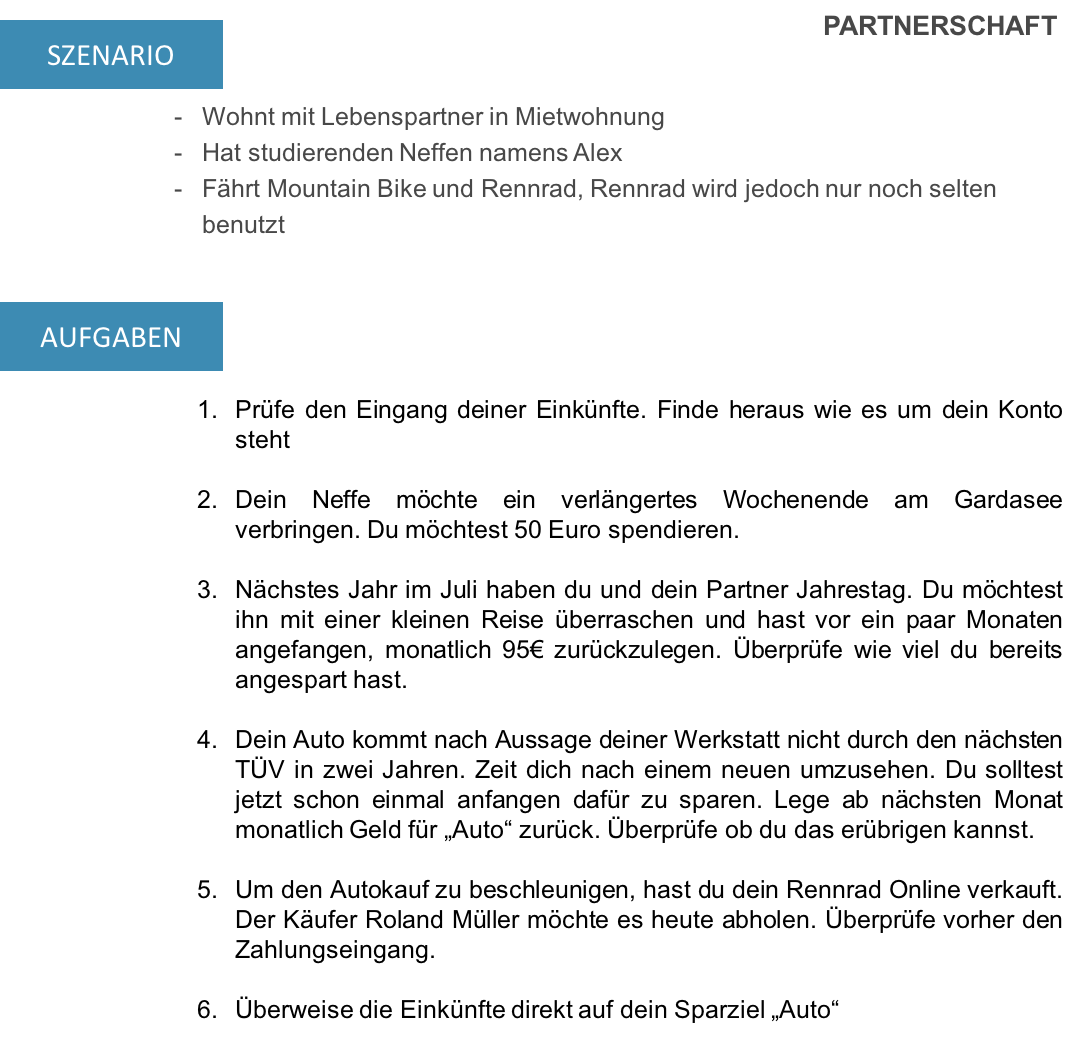
\includegraphics[width=1.0\textwidth]{bilder/3_szenarioPartner.png}}
    \caption{Partnerschaft Szenario}
    \label{fig:szenario-partner}
\end{figure}

\textbf{Verheiratet Szenario}\\
Als Vorlage dieses Szenarios wird die Persona \textit{Robert Trier} aus Abbildung \ref{fig:robert-trier} verwendet. Auch hier werden Lebensumstände, Einkommen und Hobbies für die Wahl der Aufgaben herangezogen. In Abbildung \ref{fig:szenario-verheiratet} sieht man Szenario und entsprechende Aufgaben.\\\\
Diese Szenarien sollen nun mit potentiellen Nutzern getestet werden. 

\section{Prototyping}
\label{sec:prototyping}
Im Usability Engineering wird Prototyping eingesetzt, um Produkte und Aspekte der Benutzerschnittstelle zu entwerfen, zu evaluieren und zu verbessern. Dies geschieht bevor ein lauffähiges System vorhanden ist. Beim Prototyping gibt es verschiedene Stufen. Diese beschreiben in wie weit der Prototyp dem zu entwickelnden Produkt in den folgenden Bereichen ähnelt:
\begin{itemize}
\item Funktionsumfang: Welche der vorgesehenen Funktionen der Prototyp zeigt
\item Funktionstiefe: Wie detailliert die Funktionen wiedergegeben werden
\item Darstellungstreue: Wie sehr das Erscheinungsbild dem Endprodukt ähnelt
\item Interaktivität: Wie interaktiv der Prototyp ist
\item Datengehalt: Ob dynamische oder statische Daten verwendet werden
\item Technische Reife: Wie viel der endgültigen Technologie des Endproduktes im Prototypen steckt.
\end{itemize}

Jeder Prototyp stellt einen Kompromiss zwischen notwendigem Aufwand und Zweck dar \cite{richter-ux-compact}. Anhand der aufgelisteten Bereiche, lassen sich Prototypen in die folgenden drei Stufen unterteilen:

\begin{itemize}
    \item\textit{\ac{LoFi}}: \ac{LoFi} ist vom eigentlichen Endprodukt am weitesten entfernt. Im Gegenzug ist der Kostenaufwand dieser Methode sehr gering, da meist einfachste Werkzeuge zum Einsatz kommen. Bei grafischen Oberflächen wird diese Form des Prototyping oft mit Papier und Stift angewandt. Dabei werden die einzelnen Oberflächen auf Papier skizziert. Mit diesen Papierprototypen lassen sich \zB erste Bedienkonzepte der Oberfläche testen. In einem Test navigiert die Testperson über die Papierskizzen, die von einem Helfer entsprechend der Bedienlogik ausgetauscht werden.
    
    \item\textit{\ac{MiFi}}: Interaktivität und Erscheinung eines \ac{MiFi} Prototypen sind näher am Endprodukt als \ac{LoFi}. Hier können bereits digitale, interaktive Designs von Oberflächen zum Einsatz kommen. Benötigte Daten und komplexe Funktionalität werden meist noch vorgetäuscht (engl. \textit{gemockt}).
    
    \item\textit{\ac{HiFi})}: Ein \ac{HiFi} Prototyp ist dem Endprodukt sehr ähnlich. Hier kann es sich tatsächlich um ein funktionierendes System handeln. Möglicherweise ist es im Funktionsumfang eingeschränkt oder benötigte Daten werden noch gemockt. Oft kommen dabei bereits die Technologien zum Einsatz, die Teil des zu entwickelnden Produktes sind.
\end{itemize}

Der im Zuge dieser Arbeit entwickelte Banking-Skill, kann also als ein \ac{HiFi} Prototyp bezeichnet werden. Wie bereits erwähnt, wird für die Umsetzung in Kapitel \ref{cha:umsetzung} zunächst ein Konzept ausgearbeitet. Da die Bearbeitungszeit bei der Durchführung der Arbeit ein Faktor ist, soll hierfür entweder \ac{LoFi} oder \ac{MiFi} Prototyping verwendet werden. Mit Hilfe der passenden Werkzeuge und Methoden wird das Konzept durch Tests mit potentiellen Nutzern schrittweise ausgebaut. Für die Wahl eines passenden Tools beschreibt Kapitel \ref{subsec:anforderungen-prototyping} die Anforderungen.

\subsection{Anforderungen an ein Prototyping Tool}
\label{subsec:anforderungen-prototyping}
Bevor eine passende Anwendung gewählt wird, müssen die Anforderung an diese definiert werden.
\begin{itemize}
\item Schnelle Änderungen:\\
Es ist wichtig zu erkennen was für die Nutzer funktioniert. Noch wichtiger ist früh zu erkennen was nicht funktioniert -- Stichwort \textit{fail early}. Das heißt die Anwendung soll die Möglichkeit bieten, Ideen schnell auszuprobieren und diese gegebenenfalls zu verwerfen \bzw weiterzuverfolgen. Als Folge dessen ist darauf zu achten, dass Änderungen im Konzept keine Änderungen von Quelltext nach sich ziehen.

\item Konversationsfluss entstehen lassen:\\
Die Ergebnisse der Tests sollen möglichst realitätsnah sein, um das Konzept sinnvoll zu erweitern. Um das zu erreichen, muss die Anwendung das Aufkommen eines Konversationsflusses ermöglichen. Die Anwendung ist dabei an die technischen Möglichkeiten von Alexa auszurichten. Dazu zählen die Verzögerungen zwischen der Frage einer Testperson und der entsprechenden Antwort vom System. Des Weiteren muss es möglich sein Gegenfragen zu stellen. Für die Durchführung der Aufgaben aus den Szenarien in Kapitel \ref{subsec:szenarien} ist dies essenziell. Werden beispielsweise die benötigten Informationen einer Überweisung nicht vom Nutzer eingegeben, muss das System entsprechend nachfragen.

\item Unterstützung der Sprache:\\
Der Banking Skill wird in Deutsch entwickelt. Daher ist das Verstehen von Formulierungen in deutscher Sprache notwendig. 
\end{itemize}

Im Anschluss wird eine entsprechende Anwendung gesucht. Die hier genannten Anforderungen zielen vor allem auf geringen Zeitaufwand in der Verwendung ab. Diese Tatsache lässt auf ein \ac{MiFi} Prototyping Tool schließen.

\subsection{Existierende Anwendungen}
\label{subsec:prototyping-existierende-anwendungen}
Anders als im Bereich der \ac{GUI} Entwicklung, ist die Auswahl der \ac{CUI}-\ac{MiFi}-Anwendungen überschaubar. Im Folgenden werden drei dieser Anwendungen näher betrachtet:

\begin{itemize}
    \item\textit{Sayspring}: Eine Web-Anwendung für das Entwerfen und Prototyping von \acp{VUI} ohne Programmieraufwand \cite{sayspring}.
    \item\textit{API.AI (heute Dialogflow)}: Eigentlich ein Framework für die Entwicklung von Chatbots und \acp{VUI}. Es kann auch als Prototyping Tool zweckentfremdet werden \cite{dialogflow-api-ai}. 
    \item\textit{Wit.ai}: Ähnlich wie API.AI, handelt es sich um ein Framework für die Entwicklung von Chatbots und \acp{VUI} \cite{wit-ai}.
\end{itemize}

Als Entscheidungshilfe stellt Tabelle \ref{tab:vergleich-mifi-toolauswahl} die Anforderungen aus Kapitel \ref{subsec:anforderungen-prototyping} den genannten Anwendungen gegenüber.

\begin{table}[!htb]
\centering
 \begin{tabular}{ | m{5cm} || C{2cm}| C{2cm} | C{2cm} |} 
 \hline
 Anforderungen & Sayspring & API.AI & Wit.ai
 \\
 \hhline{=::===}
 Schnelle Änderungen & \danger & \xmark & \xmark\\ \hline
 Konversationsfluss & \danger & \danger & \danger\\\hline 
 Sprachunterstützung & \xmark & \cmark & \cmark\\\hline 
\end{tabular}
\caption{Auswahlhilfe für Anwendungen aus dem \ac{CUI} Mid-Fidelity-Prototyping}
\label{tab:vergleich-mifi-toolauswahl}
\end{table}

Der Vergleich zeigt, dass keine der Anwendungen alle Anforderungen erfüllen kann.\\
Mit Sayspring kann man Konversationen schnell und einfach aufbauen, jedoch kann nur das verstanden werden was man modelliert. Ein echter Konversationsfluss kann somit nicht aufgebaut werden. Änderungen lassen sich zunächst schnell vornehmen. Bei zunehmender Komplexität wird die Bearbeitung eher mühsam. Der größte Nachteil von Sayspring ist allerdings die Sprache. Zum Zeitpunkt der Evaluierung unterstützt es lediglich englischsprachige Projekte. Deutsch wird erst seit dem 05.09.2017 unterstützt \cite{sayspring-german-support}. Abbildung \ref{fig:sayspring-gui} zeigt die Oberfläche der Web-Anwendung mit bereits erstellten Dialog Szenarien.

\begin{figure}[!htb]
    \centering
    \fbox{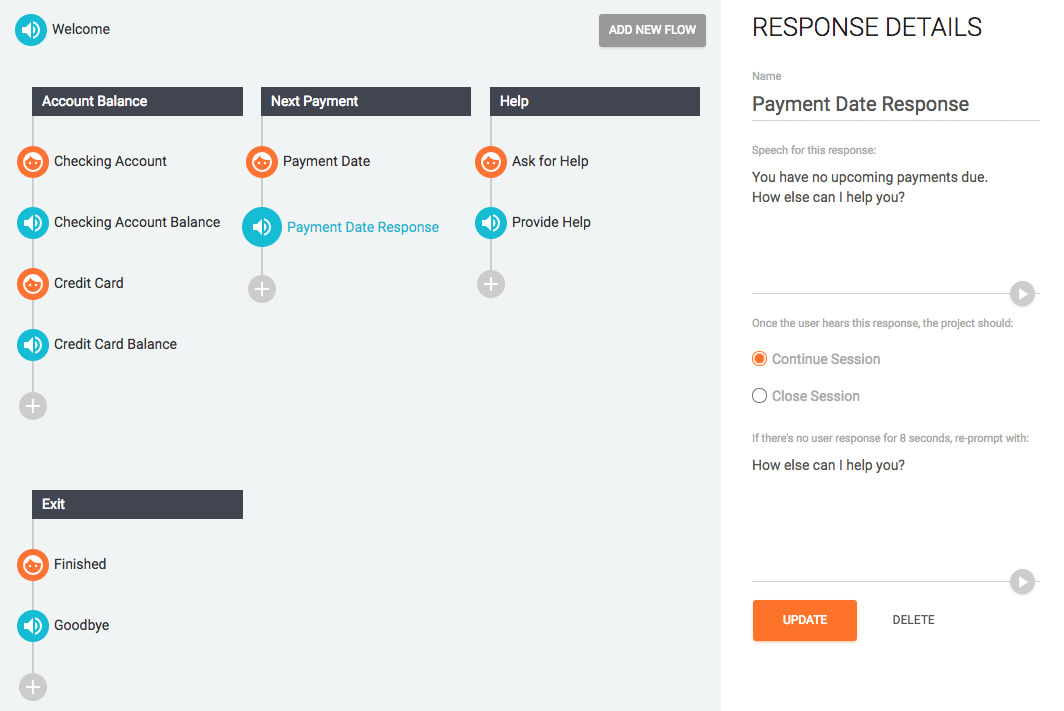
\includegraphics[width=0.8\textwidth]{bilder/3_sayspringGui.png}}
    \caption{Oberfläche der Sayspring Web-Anwendung}
    \label{fig:sayspring-gui}
\end{figure}

Anwendungen von API.AI bestehen, ähnlich wie Alexa, aus zwei Komponenten. Einer Interaction Model ähnlichen und einer Logikkomponente. Das Model muss ebenfalls mit Intents und Formulierungen konfiguriert werden. Auch wenn die Eingabe komfortabel ist sind Änderungen bei komplexen Projekten eher langsam umzusetzen. Hinzu kommt, dass die Logikkomponente implementiert werden muss. Logische Änderungen im Konzept sind also mit viel Aufwand verbunden. Auch hier kann die Konversation gut modelliert werden. Dennoch besteht hier das gleiche Problem wie bei Sayspring. Ein echter Fluss kann durch das eingeschränkte Verständnis nur schwer aufkommen.\\
Wit.ai ähnelt API.AI hinsichtlich Funktionsweise und Konfiguration über die Oberfläche. Auch hier muss Logik implementiert werden. Hervorzuheben ist, dass Wit.ai bereits zum Zeitpunkt der Evaluierung viele Sprachen unterstützt. Da keine der \ac{MiFi} Anwendungen passend erscheint, wird im folgenden Kapitel nach einer anderen Möglichkeit gesucht.

\subsection{Entstehung einer Prototyping Toolchain}
\label{subsec:prototyping-entstehung-toolchain}
Die Anwendungen aus Kapitel \ref{subsec:prototyping-existierende-anwendungen} können gemäß den Anforderungen aus Kapitel \ref{subsec:anforderungen-prototyping} nicht verwendet werden. Aus diesem Grund werden zunächst Methoden aus dem \ac{LoFi} Bereich näher betrachtet. Ähnlich wie bei der Entwicklung von \acp{GUI} kann man auch hier auf Stift und Papier zurückgreifen. Statt Oberflächen skizziert man Dialoge. Ähnlich wie ein Filmskript stellen sie Ausschnitte einer Interaktion dar \cite{pearl-design-vui}. Geschriebene Dialoge kann man mit einer einfachen Methode testen. Diese ist unter dem Namen \textit{\ac{WOz}} oder auch \textit{Wizard-of-Technique} bekannt. Bei \ac{WOz} Tests ist das eigentliche System noch nicht verfügbar. Stattdessen erweckt ein „Mensch hinter dem Vorhang“ den Eindruck eines funktionierenden Systems \cite{pearl-design-vui}. Für \ac{LoFi}-Prototyping kann ein \ac{WOz} Test gemäß Abbildung \ref{fig:woz-lofi} aufgebaut werden.

\begin{figure}[!htb]
    \centering
    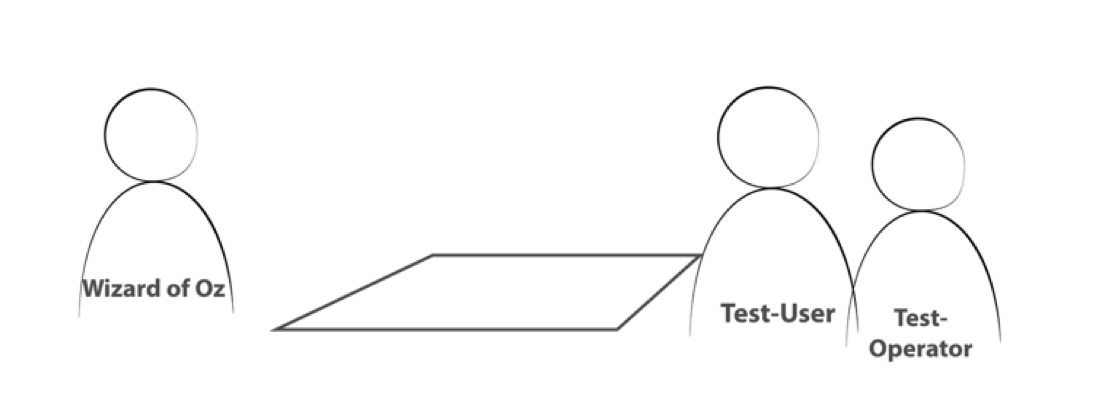
\includegraphics[width=1.0\textwidth]{bilder/3_wozLoFi.png}
    \caption{Low-Fidelity-Prototyping Test auf Basis von Wizard-of-Oz}
    \label{fig:woz-lofi}
\end{figure}

Der \ac{WOz} sitzt auf einer Seite eines Tisches, während die Testperson auf der anderen Seite sitzt. Der Test-Operator stellt der Testperson Aufgaben und betreut diese bei auftretenden Fragen. Die Testperson stellt dem \ac{WOz} für die Erfüllung der Aufgaben Fragen, die der \ac{WOz} entsprechend dem vorher festgelegten Skript beantwortet. Der Operator macht dabei Notizen zur Durchführung, dem Verlauf und den Ergebnissen des Tests.\\
Dieser Aufbau bringt Probleme mit sich. Der \ac{WOz} erhält über mehrere Kanäle Informationen, die dem Endprodukt nicht zur Verfügung stehen. Er kann die komplette Unterhaltung zwischen der Testperson und dem Operator mithören. Dadurch ist es möglich Schlüsse aus dem Kontext der Unterhaltung zu ziehen, die über das eigentliche Sprachkommando hinaus gehen. Weiterhin kann der \ac{WOz} den Fluss der Konversation durch Lachen oder Versprechen negativ beeinflussen. Er erhält weitere Informationen aus Mimik und Gestik der Testperson. Durch Aufstellen einer Trennwand kann man dem Problem entgegen wirken. Denkbar ist auch, den \ac{WOz} räumlich von den anderen Personen zu trennen. Abbildung \ref{fig:woz-lofi-voip} zeigt einen solchen Aufbau, in dem die Räume über Rechner mit \textit{\ac{VoIP}}-Anwendungen wie \zB Skype\footnote{https://www.skype.com/en, Abgerufen 31.10.2017} oder Google Hangout\footnote{https://hangouts.google.com, Abgerufen 31.10.2017} verbunden. 

\begin{figure}[!htb]
    \centering
    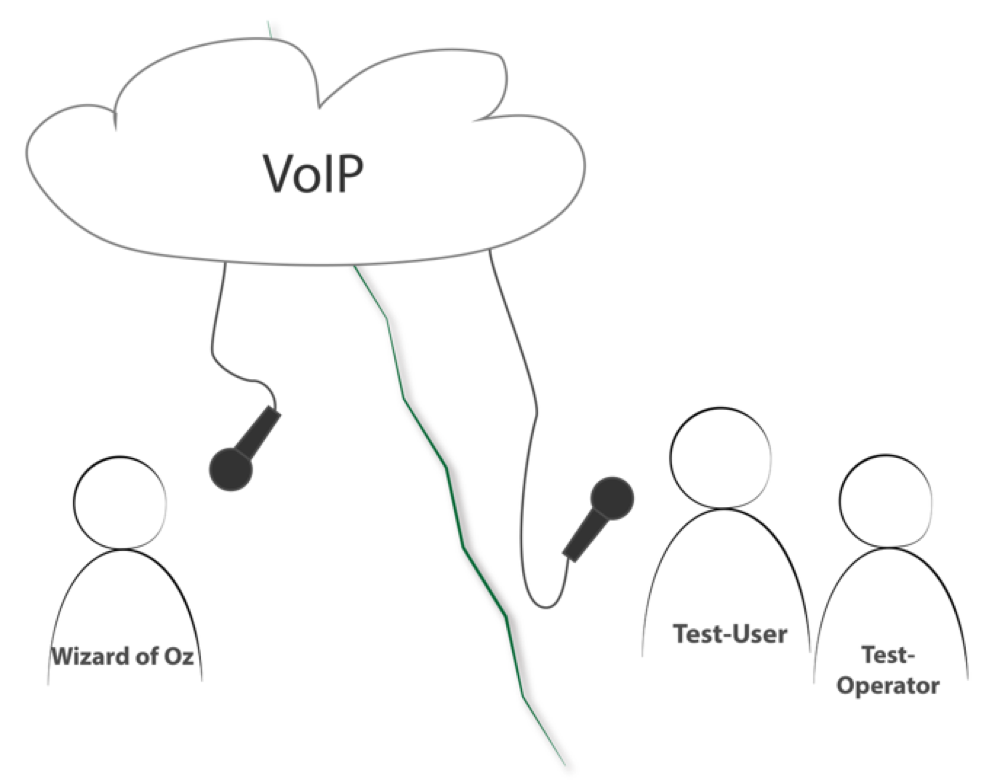
\includegraphics[width=0.8\textwidth]{bilder/3_wozLoFiVoIP.png}
    \caption{Wizard-of-Oz Low-Fidelity-Prototyping mit Voice over IP}
    \label{fig:woz-lofi-voip}
\end{figure}

Werden etwaige Kameras an den Rechnern deaktiviert, gibt es keine Informationen bezüglich Mimik und Gestik. Unter Einsatz eines Mikrofons mit Taster für die Sprachaktivierung sind auch die Unterhaltungen der Testperson und des Operators nicht zu hören. Diese Methode bringt viele Vorteile mit sich. Neben dem geringen Kosten- und Geräteaufwand, ist es zudem nicht nötig komplexe Technologien wie \ac{ASR} und \textit{NLP} zu verwenden oder gar zu implementieren. Da der \ac{WOz} ein Mensch ist, kann er alle Formulierungen der Testperson verstehen. Es besteht aber die Möglichkeit, dass sich der Wizard verspricht, lachen muss oder Sätze aus dem Skript nicht finden kann. Weitere Nachteile sind die zeitintensive Erstellung, Verwaltung und Erweiterung der Skripten. Bei zunehmender Komplexität wird es also schwieriger die Rolle des \ac{WOz} einzunehmen. Ein reibungsloser Ablauf ist wahrscheinlich mit intensiver Einarbeitung in das Skript verbunden. Werden die verbleibenden Probleme behoben, könnten mit diesem System sämtliche Anforderungen aus Kapitel \ref{subsec:anforderungen-prototyping} erfüllt werden. Abbildung \ref{fig:woz-weiterentwicklung} zeigt eine mögliche Weiterentwicklung dieser Gedanken.

\begin{figure}[!htb]
    \centering
    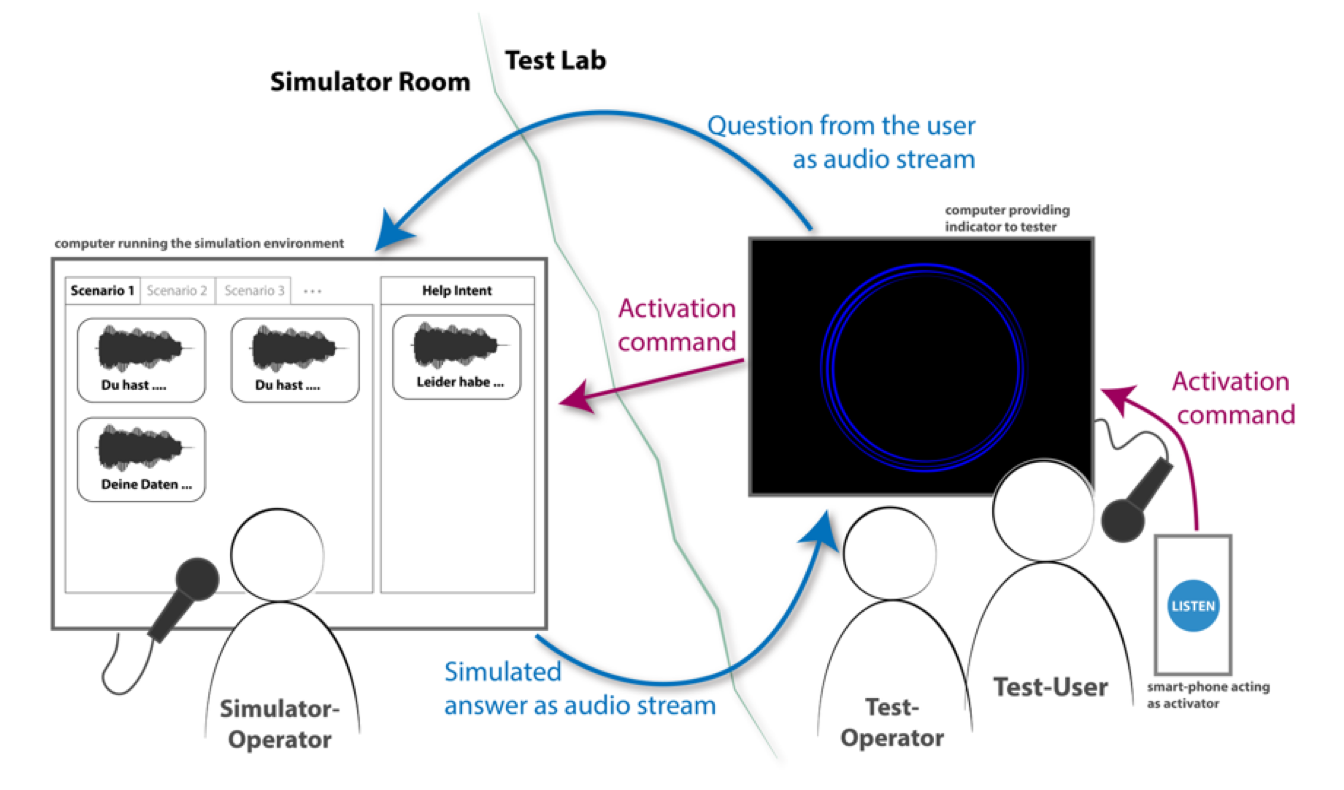
\includegraphics[width=1.0\textwidth]{bilder/3_wozFinal.png}
    \caption{Weiterentwicklung des Wizard-of-Oz Testaufbaus}
    \label{fig:woz-weiterentwicklung}
\end{figure}

Nach wie vor spricht die Testperson nach Aktivierung in ein Mikrofon und überträgt das Gesprochene an den \ac{WOz}. Dieser spricht die Antwortsätze nicht mehr selbst in ein Mikrofon. Er spielt zum richtigen Zeitpunkt vorher aufgenommene oder erzeugte Antwortsätze über eine Oberfläche ab. Diese werden als Audio an die Testperson im Labor übertragen. Bei entsprechender Gestaltung der Oberfläche findet sich der \ac{WOz} auch bei komplexen Tests zurecht. Gemäß Abbildung \ref{fig:woz-weiterentwicklung} lassen sich die Antworten in verschiedene Reiter unterteilen. Die gezeigte \ac{GUI} löst damit unter Umständen das Problem des Zurechtfindens und des Versprechens. Das Erstellen und vor allem schnelle Ändern des Dialog Skriptes sind nach wie vor kritisch. Zusätzlich zu der gezeigten Anwendung werden also noch weitere benötigt, die den Ablauf des Dialoges modellieren können und die Antwortsätze als Audio generieren. Das Ergebnis dieses Gedankens ist die in Abbildung \ref{fig:prototyping-toolchain} gezeigte Toolchain\footnote{Die Toolchain ist in Zusammenarbeit mit Steffen Blümm, dem fachlichen Betreuer der Arbeit entstanden}.

\begin{figure}[!htb]
    \centering
    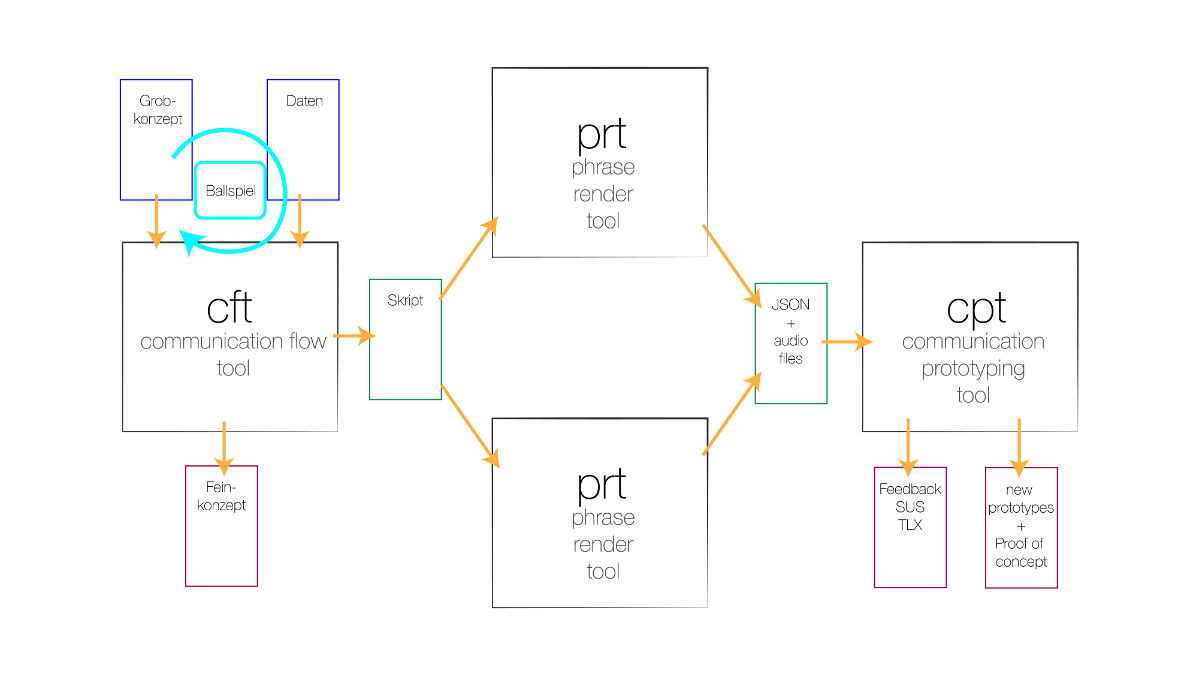
\includegraphics[width=1.0\textwidth]{bilder/3_toolchain-final.png}
    \caption{Prototyping Toolchain}
    \label{fig:prototyping-toolchain}
\end{figure}

Zunächst wird über ein Ballspiel ein Grobkonzept erarbeitet. Mit Hilfe eines Datensatzes (hier \zB Bank"~ \bzw Umsatzdaten) können sich zwei Personen gegenseitig einen „Ball“ zuwerfen. Das heißt abwechselnd die Rolle des Systems und des Benutzers einnehmen und dabei mögliche Fragen- und Antwortszenarien durchspielen. Das Ballspiel kann auch durch andere Methoden ersetzt werden, um ein Grobkonzept auszuarbeiten. Dieses Konzept wird händisch in das \textit{\ac{cft}} eingegeben. Hier können die Dialoge digital erstellt und bearbeitet werden. Denkbar für das \ac{cft} ist eine Sayspring ähnliche Oberfläche (\vgl Abbildung \ref{fig:sayspring-gui}). Im nächsten Schritt gibt das \ac{cft} den Dialogfluss in Form eines Datensatzes (\zB  in \textit{\ac{JSON}} Format) aus. Diese Ausgabedatei wird in das \textit{\ac{prt}} geladen. Es konvertiert gemäß der \ac{cft} Ausgabe die Antwortsätze über eine Art \ac{TTS} Synthese in Audio Dateien und reicht den \ac{cft} Datensatz weiter. Im letzten Schritt baut sich die \ac{WOz} Oberfläche mit Hilfe der \ac{prt} Ausgabe auf. Die generierten Audio Dateien und Szenarien werden geladen und der Test kann starten. Mit den Erkentnissen aus dem durchgeführten Test kann nun das Konzept über das \ac{cft} angepasst und ein weiterer Testlauf gestartet werden. Diese Vorgehensweise ist ein iterativer Prozess, der beliebig oft wiederholt werden kann. Aus dem Grobkonzept entsteht ein Feinkonzept, dass als Basis für die Implementierung genutzt wird.

\subsection{Umsetzung der Prototyping Toolchain}
\label{subsec:umsetzung-prototyping-toolchain}
Im Folgenden wird die Umsetzung der Prototyping Toolchain aus Abbildung \ref{fig:prototyping-toolchain} beschrieben. Da für die Durchführung der Tests vor allem das communication prototyping tool von Bedeutung ist, wird die Toolchain von rechts nach links entwickelt.\\

\textbf{communication prototyping tool}\\
Um den Zeitaufwand in Grenzen zu halten, ist das \ac{cpt} mit \textit{Max} von Cycling74 \cite{max-msp} umgesetzt, eine Art digitales Baukasten System. Max verbindet Objekte über virtuelle Leitungen, um interaktive Audio"~ und Grafiksysteme zu erstellen. Projekte in Max sind in sogenannten \textit{Patchern} organisiert. Sie beinhalten die verknüpften Objekte und sind ineinander verschachtelbar.\\
Das \ac{cpt} wird mit Max nach der Vorlage aus Abbildung \ref{fig:woz-weiterentwicklung} umgesetzt. Gemäß der Aufteilung in Simulator-Raum und Testlabor gibt es zwei Oberflächen \bzw Patcher, die auf den jeweiligen Rechnern laufen und Daten austauschen. Diese werden im Folgenden als \textit{Simulator-Panel} und \textit{Tester-Panel} bezeichnet. Abbildung \ref{fig:cpt-komponenten} zeigt eine Übersicht der Panele mit ihren Komponenten. 

\begin{figure}[!htb]
    \centering
    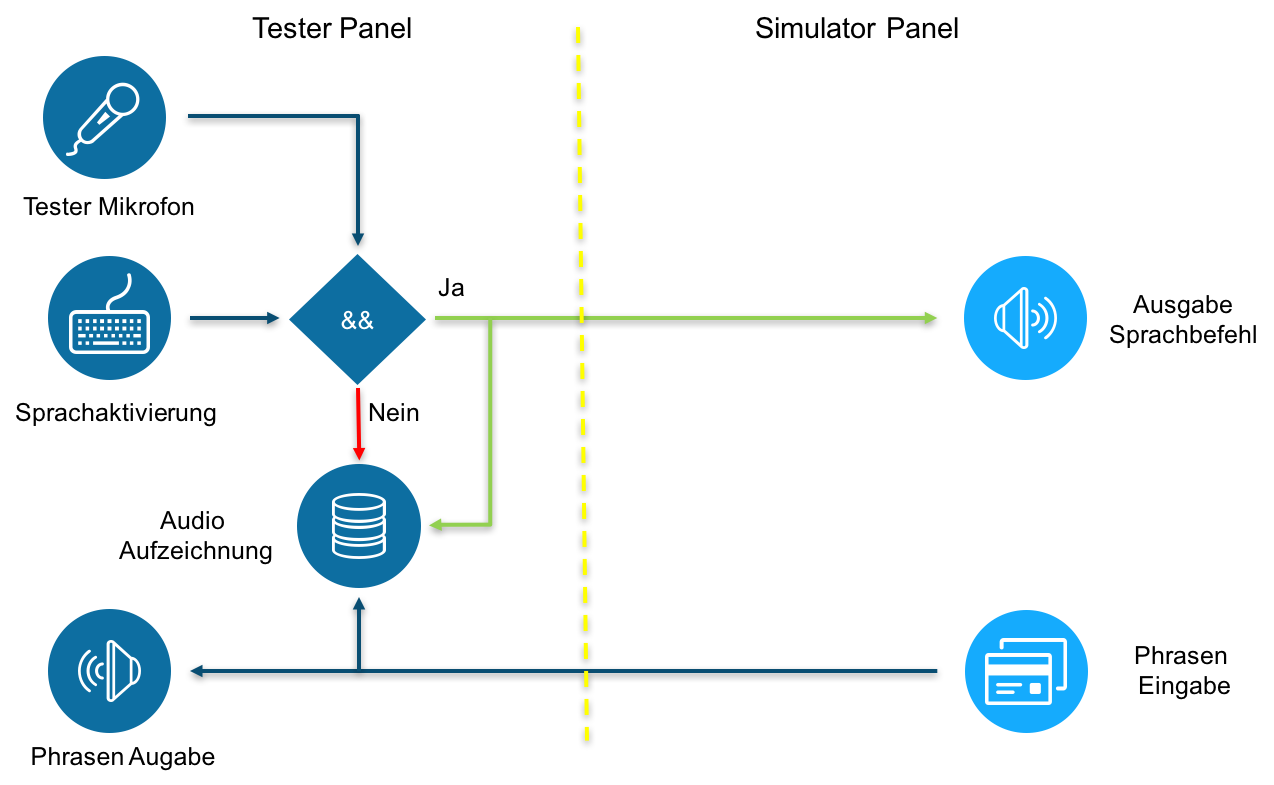
\includegraphics[width=1.0\textwidth]{bilder/3_cptKomponenten.png}
    \caption{Komponentenübersicht des Tester- und Simulator-Panels}
    \label{fig:cpt-komponenten}
\end{figure}

Das Tester-Panel ist für die Übertragung der Sprachbefehle des Testers und einer Möglichkeit der Sprachaktivierung zuständig. Zudem gibt es die Antwortphrasen aus, die vom Simulator-Panel übertragen werden. Diese Seite bildet die \ac{WOz} Oberfläche ab, die gemäß des Szenarios dynamisch aufgebaut wird. Sie gibt die Sprachbefehle des Testers aus und ermöglicht es diesem zu Antworten. Man greift dabei auf die generierten Audiodateien zurück. Um die Tests besser nachvollziehen zu können, werden zwei Audiospuren aufgenommen. Eine dieser Spuren zeichnet alles über das Tester Mikrofon (auch ohne Sprachaktivierung) und den Antwortphrasen auf. Die andere Spur zeichnet lediglich die Konversation zwischen Tester (mit Sprachacktivierung) und \ac{WOz} auf, um eine differenzierte Perspektive der Unterhaltung darzustellen. Im Folgenden ist die Umsetzung der Oberflächen in Max dokumentiert. Da der Fokus der Arbeit ein anderer ist, wird hier nur ein kurzer Überblick gegeben. Das komplette System mit den entsprechenden Quelltexten ist auf der CD unter \textit{„Quelltexte/cpt/“} zu finden. Abbildung \ref{fig:cpt-tester-panel} zeigt den Max Patcher für das Tester-Panel. 

\begin{figure}[!htb]
    \centering
    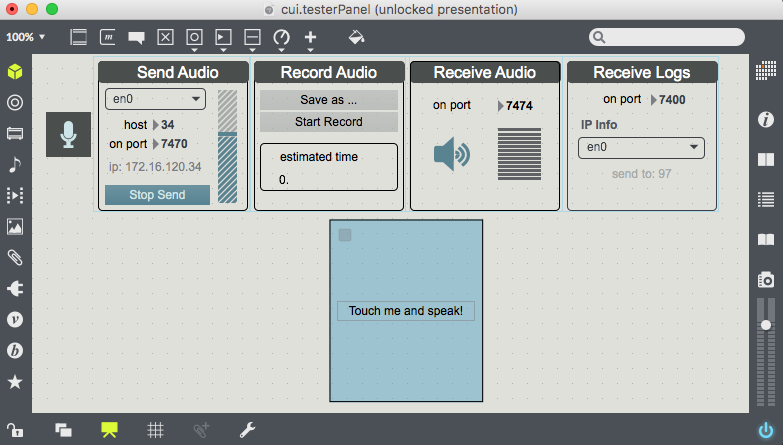
\includegraphics[width=1.0\textwidth]{bilder/3_cptTester.png}    
    \caption{Max Oberfläche mit dem cpt Tester-Panel}
    \label{fig:cpt-tester-panel}
\end{figure}

\textbf{Tester-Panel}\\
Hier sind die verschiedenen Komponenten aus Abbildung \ref{fig:cpt-komponenten} zu sehen. \textit{Send Audio} überträgt die Spracheingaben vom Mikrofon des Rechners an die konfigurierte \textit{\ac{IP}}-Adresse. \textit{Record Audio} zeichnet die Tonspuren auf. Der blau hinterlegte, darunterliegende Bereich bildet die Sprachaktivierung ab. Über die \textit{Receive Audio} Komponente empfängt man die Antwortphrasen des Simulator-Panels. Über die \textit{Logging Komponente} können zusätzliche Textinformationen zum Test gespeichert werden. Das Simulator-Panel, zu sehen in Abbildung \ref{fig:cpt-simulator-panel}, beinhaltet die Gegenstücke zu den eben genannten Komponenten. 

\begin{figure}[!htb]
    \centering
    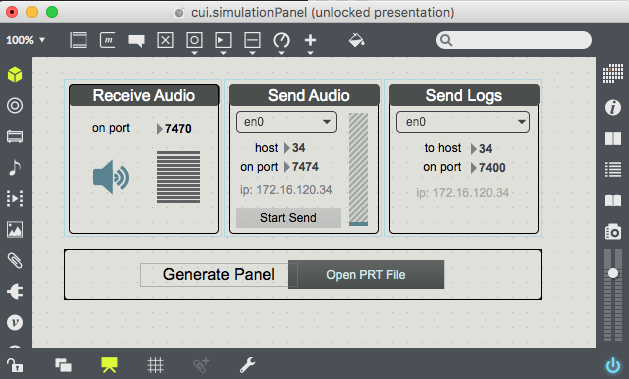
\includegraphics[width=1.0\textwidth]{bilder/3_cptSimulator.png}
    \caption{Max Oberfläche mit dem cpt Simulator-Panel}
    \label{fig:cpt-simulator-panel}
\end{figure}

\textbf{Simulator-Panel}
\textit{Receive Audio} empfängt die Spracheingaben des Testers, während die \textit{Send Audio} Komponente die Antwortphrasen zurück sendet. Über die darunter liegende Schaltfläche kann eine \ac{prt} Ausgabe Datei (\vgl Abbildung \ref{fig:prototyping-toolchain}) geladen werden. Die Oberfläche baut sich im Anschluss dynamisch auf. Dieser Vorgang ist mit entsprechenden Abbildungen in Kapitel \ref{subsec:prototyping-tests} näher beschrieben. Vor Verwendung des \ac{cpt}, müssen zunächst die Audio und Skript Dateien entsprechend generiert werden.\\

\textbf{Skript Datei}\\
Das Skript dient als Mittel zur Kommunikation zwischen den Anwendungen der Toolchain. Als Format wird \textit{\ac{JSON}} verwendet. Im \nameref{sec:Anhang} unter Kapitel \ref{sec:cpt-input-schema} ist das Schema des Skriptes zu finden. Es enthält strukturelle Elemente, wie den Namen des Projektes und des verwendeten Szenarios. Zudem beinhaltet es testspezifische Daten, wie die Namen der Testpersonen und den eigentlichen Dialog-Daten mit den Antworttexten. Diese Daten bilden ein Gesamtszenario ab (hier die erarbeiteten Szenarien aus Kapitel \ref{subsec:szenarien}). Dabei unterscheidet sich die vom \ac{cft} generierte Datei kaum von der aus dem \ac{prt} ausgegebenen. 

\textbf{phrase render tool}\\
Das \ac{prt} wurde vom fachlichen Betreuer der Arbeit implementiert. Abbildung \ref{fig:prt-gui} zeigt die Oberfläche der Anwendung. Über die \textit{Start} Schaltfläche kann das vom \ac{cft} ausgegebene Skript geladen werden. Die Anwendung generiert die entsprechenden Audiodateien und komplettiert die Skript Datei. Es fügt diesem die Pfade der Audiodateien hinzu und modifiziert gegebenenfalls die Antworttexte passend zum generierten Audio. Im Anschluss werden auf der Festplatte die Ordnerstruktur entsprechend des Skriptaufbaus erstellt und sämtliche Dateien darunter abgelegt. 

\begin{figure}[!htb]
    \centering
    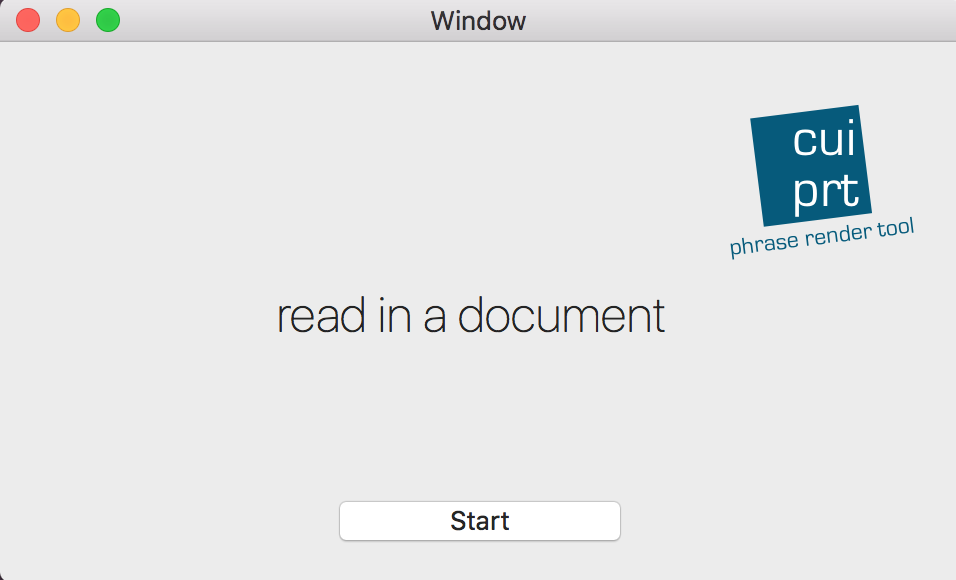
\includegraphics[width=0.7\textwidth]{bilder/3_prtGui.png}
    \caption{prt Oberfläche}
    \label{fig:prt-gui}
\end{figure}

Eine unter \textit{macOS} ausführbare Datei ist auf der beiliegenden CD unter \textit{„Quelltexte/prt/“} zu finden.

\textbf{communication flow tool}\\
Aus zeitlichen Gründen und da es für die Durchführung der Tests nicht zwingend notwendig ist, wird das \ac{cft} nicht im Zuge dieser Arbeit umgesetzt. Daher werden die Szenarien aus Kapitel \ref{subsec:szenarien} händisch in die entsprechenden Skript Dateien transkribiert. Das nächste Kapitel beschreibt die Anwendung der Prototyping Toolchain.

\subsection{Anwendung der Prototyping Toolchain}
\label{subsec:prototyping-tests}
Für die Erarbeitung eines Feinkonzeptes wird die Toolchain für den Aufbau der Benutzertests angewandt. Aufgrund es fehlenden \ac{cft} wird für jedes Szenario aus Kapitel \ref{subsec:szenarien} ein Skript per Hand erstellt. Alle Skripten sind auf der CD unter \textit{„Quelltexte/prototyping\_skripten“} zu finden. Da diese bereits Utterances und Antwortsätze enthalten, fungieren sie als das Grundkonzept und werden durch die Tests erweitert \bzw angepasst.  

\textbf{Testaufbau}\\
Vor jedem Durchlauf wird die Testperson gemäß Lebensumstand einem der Szenarien aus Kapitel \ref{subsec:szenarien} zugeordnet und ihr Name in das Skript eingetragen. Als Beispiel wird das „Partnerschafts“ Szenario aus Abbildung \ref{fig:szenario-partner-anhang} herangezogen. Aus Platz- und Übersichtsgründen ist hier eine vollständige Abbildung nicht möglich. Um den Prozess zu veranschaulichen, dient ein Skriptauszug aus der ersten Aufgabe dieses Szenarios:

\begin{center}
\textit{Prüfe den Eingang deiner Einkünfte.}
\end{center}

Aus dem Schema unter Kapitel \ref{sec:cpt-input-schema} ist bekannt, dass sich das Skript aus Teilszenarien zusammensetzt. Diese beinhalten wiederum Intents. Jeder Intent hat eine oder mehrere Antworten. Listing \ref{lst:skriptauszug-gehalt} zeigt den Skriptauszug für die Beispielaufgabe. 

\begin{lstlisting}[language={HTML},caption={Auszug aus dem Skript des Partnerschaft Szenarios},label={lst:skriptauszug-gehalt}]
{
    "name": "salaryIntent",
    "utterances": ["Gehalt/Lohn da?"],
    "priority": { "main": 0 },
    "responses": [{
            "subject": "SalaryArrived",
            "phrase": "Dein Gehalt fuer diesen Monat ist bereits eingegangen"
        }
    ]
}
\end{lstlisting}

Startet man nun das \ac{prt} und lädt die Skript Datei über die entsprechende Schaltfläche (\vgl Abbildung \ref{fig:prt-gui}), generiert es die Dateien und Ordner gemäß der Schema Struktur, zu sehen in Abbildung \ref{fig:prt-files}.

\begin{figure}[!htb]
    \centering
    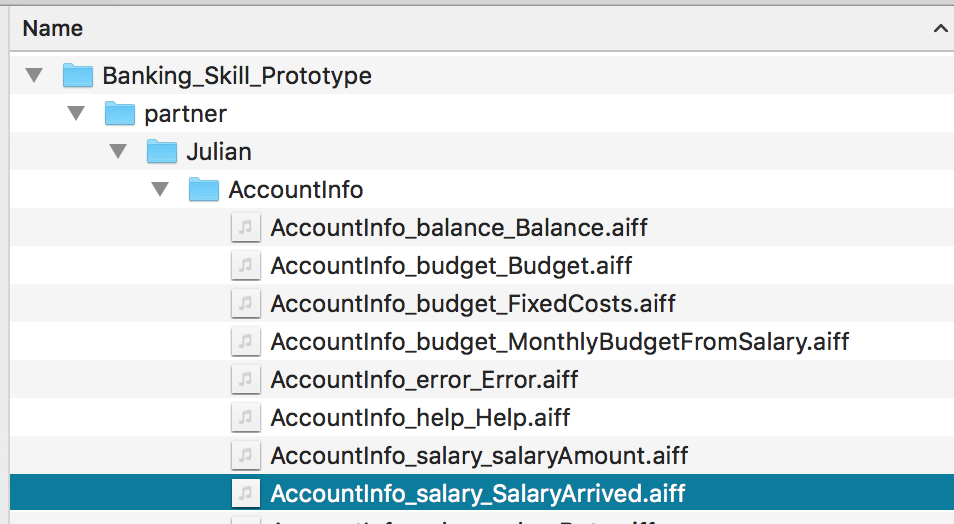
\includegraphics[width=1.0\textwidth]{bilder/3_prtAudio.png}
    \caption{Generierte Ordnerstruktur und Dateien für Partnerschafts Szenario}
    \label{fig:prt-files}
\end{figure}

Der „AccountInfo“ Ordner aus Abbildung \ref{fig:prt-files} enthält alle Audio Dateien für das erste Teilszenario. Die Datei aus dem Beispiel ist blau markiert. \newpage

\begin{lstlisting}[language={HTML},caption={Beispiel-Abschnitt nach der Modifikation durch das prt},label={lst:skriptauszug-gehalt-modifiziert}]
{
          "name" : "salaryIntent",
          "utterances": ["Gehalt/Lohn da?"],
          "priority" : {"main": 0},
          "responses" : [{
              "subject": "SalaryArrived",
              "audio": "AccountInfo_salary_SalaryArrived.aiff",
              "phrase": "Dein Gehalt fuer diesen Monat  ist bereits eingegangen"
            }
          ]
        }
\end{lstlisting} 

Auf gleicher Ebene wie der „AccountInfo“ Ordner, befindet sich das vom \ac{prt} modifizierte Skript. Listing \ref{lst:skriptauszug-gehalt-modifiziert} stellt den geänderten Abschnitt des „salaryIntent“ dar.\\ 
Der Antwortphrase wird vom \ac{prt} das Feld „audio“ hinzugefügt, welches den Namen der entsprechenden Datei enthält (\vgl Abbildung \ref{fig:prt-files}). Nun kann das \ac{cpt} gestartet und die modifzierte Skript Datei geladen werden (\vgl Abbildung \ref{fig:cpt-simulator-panel}), um die Oberfläche für den Test aufzubauen. Für jedes Teilszenario wird ein Reiter erstellt. Diese beinhalten im Idealfall alle Intents die der Tester für die Erfüllung der Aufgabe braucht oder eventuell benutzt. Abbildung \ref{fig:cpt-gui} zeigt den Auschnitt des „AccountInfo“ Reiters der für das Testen der ersten Aufgabe des Partnerschafts Szenarios verwendet wird. Darin zu sehen sind der salaryIntent und dessen Antwortphrase aus dem Beispiel. Durch Klicken auf die Antwort wird diese abgespielt und an das Tester-Panel übertragen. Rechts neben dem hier gezeigten Reiter ist ein weiterer, der alle Intents der zweiten Aufgabe enthält und so weiter.

\begin{figure}[!htb]
    \centering
    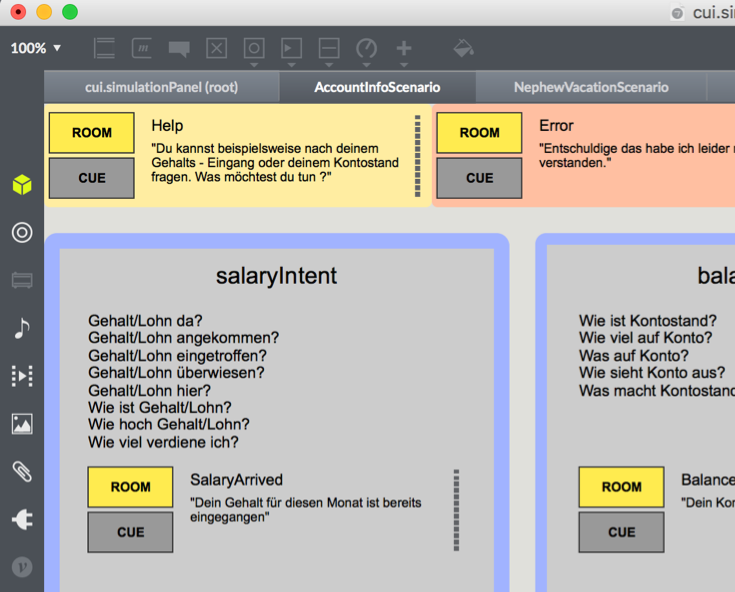
\includegraphics[width=1.0\textwidth]{bilder/3_cptGui.png}
    \caption{cpt GUI für das Testen der ersten Aufgabe im Partnerschaft Szenario}
    \label{fig:cpt-gui}
\end{figure}

Im Testlabor muss das Tester-Panel geöffnet werden. Im Idealfall weiß die Testperson nichts vom Simulator-Panel oder der Person die es steuert. Beide Panele werden mit der \ac{IP}-Adresse des jeweils anderen Rechners und dem entsprechenden Port konfiguriert. Der Aufbau ist damit abgeschlossen und der eigentliche Test kann durchgeführt werden.\\

\textbf{Test Durchführung}\\
Der Testoperator unterweist die Testperson und stellt das Szenario vor. Im Anschluss führt der Tester die vom Operator genannten Aufgaben aus. Abbildung \ref{fig:test-user-woz} zeigt eine der Testpersonen und den im Nebenraum sitzenden \ac{WOz} bei der Durchführung eines Tests.

\begin{figure}[!htb]
  \centering
  \begin{minipage}[b]{0.48\textwidth}
    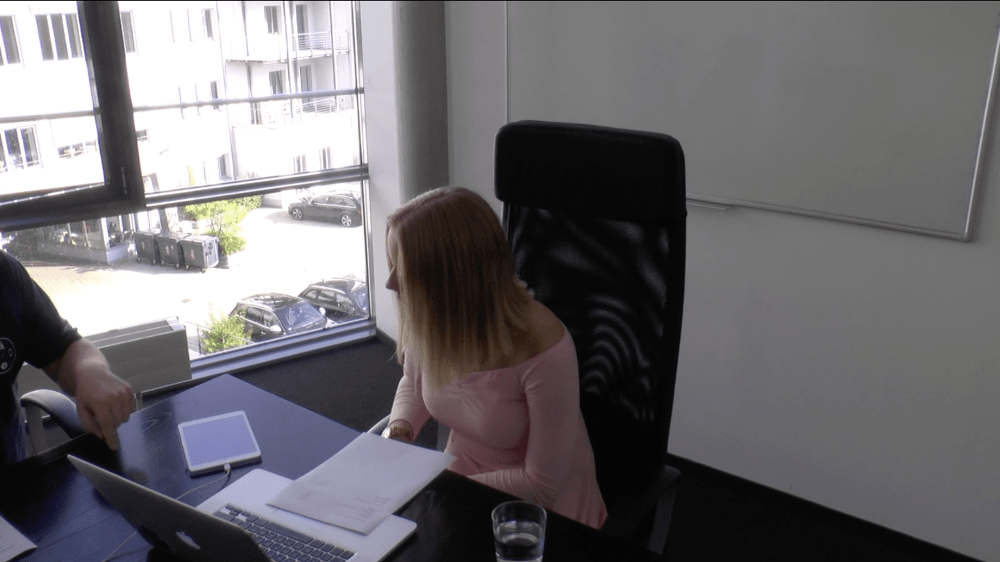
\includegraphics[width=\textwidth]{bilder/3_testUser.png}
  \end{minipage}
  \begin{minipage}[b]{0.48\textwidth}
    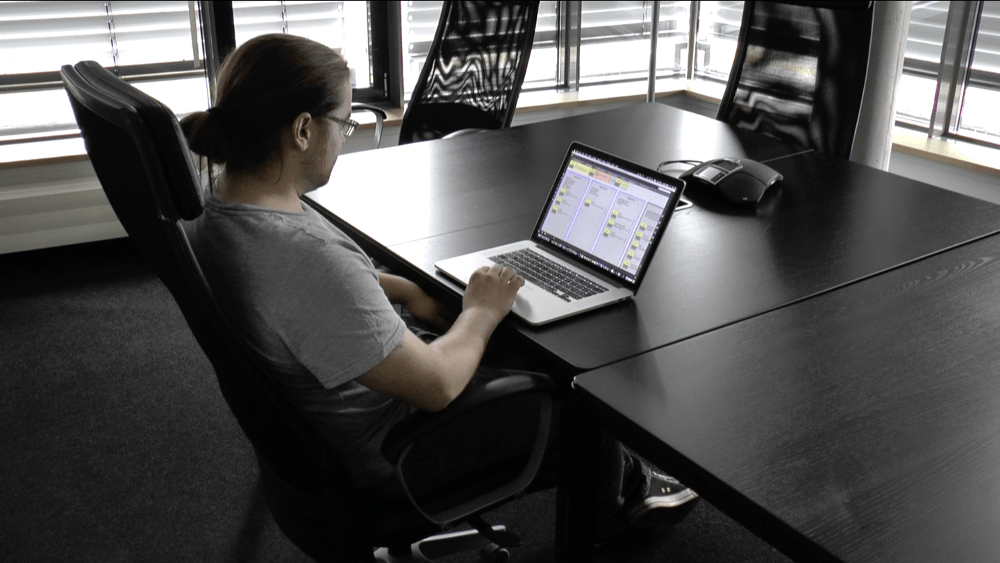
\includegraphics[width=\textwidth]{bilder/3_testWoz.png}
  \end{minipage}
  \caption{Testperson und WOz bei der Durchführung eines Tests}
  \label{fig:test-user-woz}
\end{figure}

Währenddessen notieren der Operator und \ggf der \ac{WOz} Auffälligkeiten und Anmerkungen zum Ablauf. Nach Abschluss der Aufgaben kann der Tester befragt oder das System diskutiert werden. Die Auswertung der Aufnahmen und Notizen erfolgt im Anschluss. Gewonnene Erkenntnisse fließen in die nächste Iteration ein.

\textbf{Test Ergebnisse}\\
Zwölf verschiedene Personen haben die Tests durchgeführt. Obwohl viel Zeit in die Anforderungsanalyse aus Kapitel \ref{sec:requirements-engineering} geflossen ist, hat jeder Test wichtige und sinnvolle Erkenntnisse erschlossen. Darunter auch neue Funktionalitäten, die den User Stories unter Kapitel \ref{sec:anhang-user-stories} hinzugefügt werden.. Im Folgenden wird eine Zusammenfassung gegeben.

\begin{itemize}
 \item Budget der letzten Finanzperiode: Neben der Ausgabe des Budgets der aktuellen Finanzperiode, kann auch das der letzten ausgegeben werden. Denkbar ist auch ein Vergleich beider Budgets. Dadurch ist es Nutzern möglich herauszufinden mit welcher Tendenz zu rechnen ist oder ob Anpassungen im Ausgabeverhalten bereits Wirkung zeigen.
 
 \item Ausgaben der letzten Finanzperiode: Tester haben nach den Ausgaben der letzten Finanzperiode gefragt. Dabei sollen nicht nur Fixkosten, sondern alle Ausgaben einkalkuliert werden.
 
 \item Sparziele ausgeben: Neben der Verwaltung soll es auch möglich sein alle Sparziele auszugeben.
 
 \item Fixkosten: Neben der Höhe der Fixkosten haben Tester auch gefragt, woraus sich die Fixkosten zusammen setzen. Eine Auflistung aller regelmäßigen Ausgaben ist denkbar.
 
 \item Transaktion mit IBAN: In Kapitel \ref{subsec:user-stories} ist konzipiert, dass Transaktion nur über vorher angelegte Vorlagen durchgeführt werden können. Bei Verwendung eines \ac{IBAN}, sollen Benutzer auf eine grafische Anwendung \bzw Überweisungsträger zurückgreifen. Eine der Testpersonen trägt eine Gleitsichtbrille. Sie hat folgendes sinngemäß angegeben: 
 \textit{Möchte man eine \ac{IBAN} von einem Blatt Papier, zum Beispiel einer Rechnung, ablesen und unter Verwendung einer Online-Banking-Anwendung eingeben, ist das ständige Hin- und Herwechseln zwischen Papier und Bildschirm unangenehm. Es wäre wesentlich einfacher die \ac{IBAN} vom Papier abzulesen und einem Gerät zu diktieren. Dabei muss man nicht einmal die Augen vom Papier abwenden}.
 
 \item Höhe und Überweisungsdatum des Gehaltes prüfen: Neben der Information, ob das Gehalt bereits überwiesen wurde, haben viele der Tester nach der Höhe des Gehaltes gefragt. Auch das Überweisungsdatum scheint von Interesse zu sein.
\end{itemize}

Die hier erlangten Ergebnisse zeigen, wie wichtig der Einsatz von Prototyping ist.\\
Das über die Tests iterativ entwickelte Konzept soll nun in eine einheitliche, schriftliche Form gebracht werden. Da ein Alexa Skill gemäß Kapitel \ref{sec:alexa-voice-service} in Intents organisiert ist, wird das Konzept auch auf diese Weise dokumentiert. Jeder Intent wird nach aktuellem Kenntnisstand identifiziert und über dessen Slots, in den empirischen Daten und Tests gesammelten Utterances und Antwort-Beispielen definiert. Aus Gründen der Übersichtlichkeit und Lesbarkeit, wird nur einer dieser Intents beschrieben.

\begin{figure}[!htb]
    \centering
    \fbox{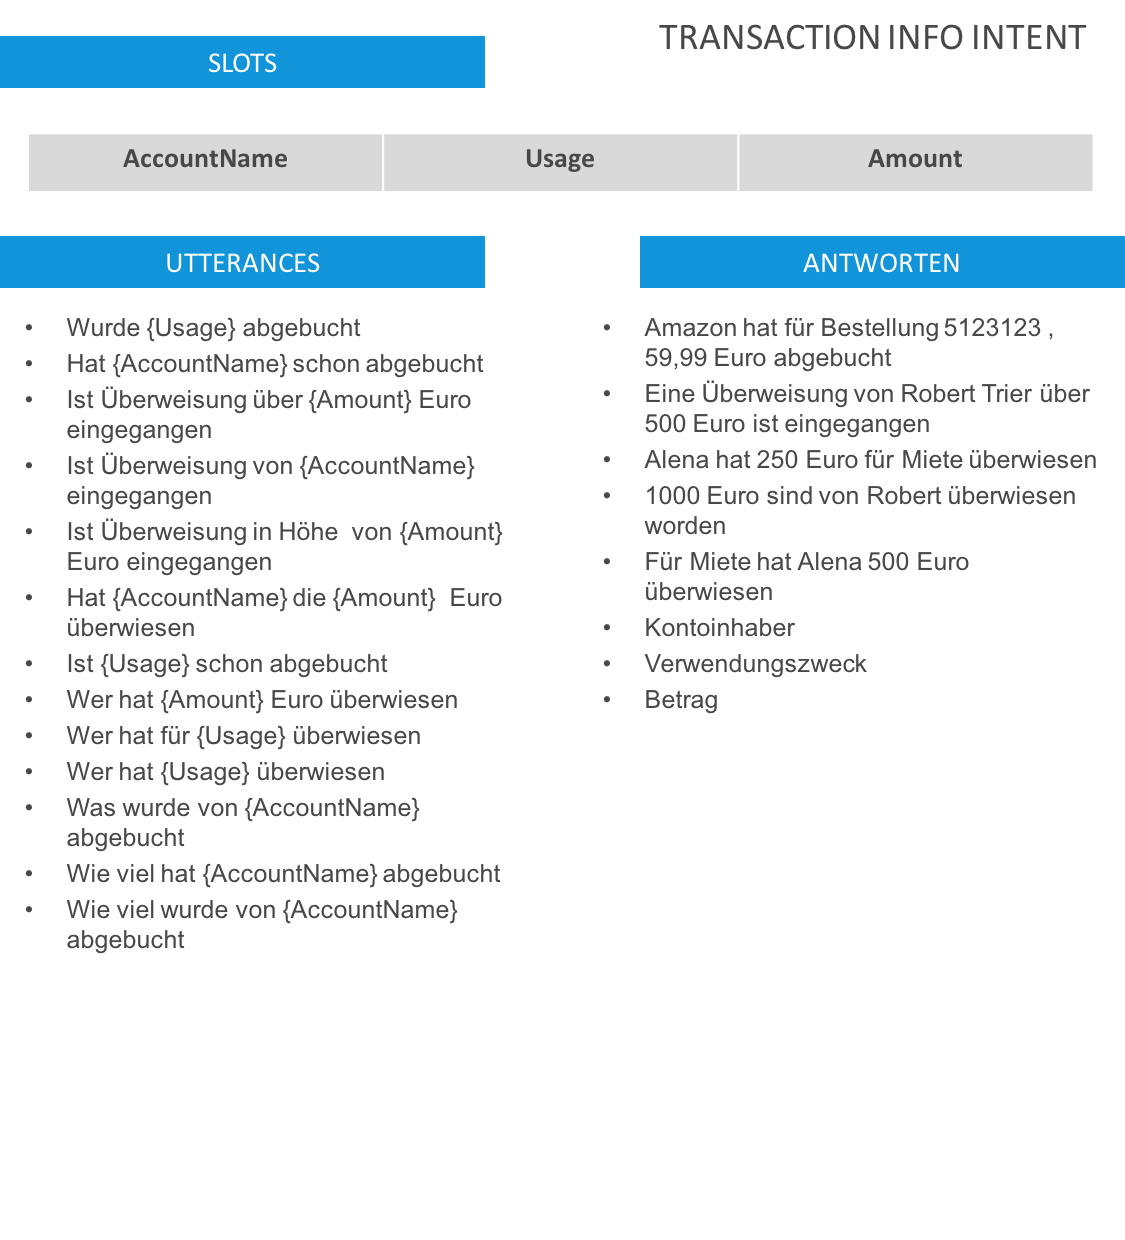
\includegraphics[width=1.0\textwidth]{bilder/3_conceptTransactionInfo.png}}
    \caption{Ausgearbeiteter Transaktions-Info Intent}
    \label{fig:conception-transaction-info}
\end{figure}

Sämtliche Intents sind im Anhang unter Kapitel \ref{sec:anhang-konzept} zu finden. Abgesehen von etwaigen Änderungen die für die Umsetzung notwendig sind, wird das Konzept im weiteren Verlauf der Arbeit nicht weiter ausgebaut. An dieser Stelle sei jedoch erwähnt, dass das Bedienkonzept einer \ac{CUI} Anwendung auch lange nach der Auslieferung intensiv erweitert werden muss. Die hier erarbeiteten Formulierungen bilden lediglich eine kleine Basis dessen ab, was der Skill verstehen sollte. Abbildung \ref{fig:conception-transaction-info} zeigt die Ausarbeitung des „TransactionInfoIntent“. Gemäß Kapitel \ref{sec:ziel-der-arbeit}, werden Teile dieses Konzeptes in Kapitel \ref{cha:umsetzung} umgesetzt.\\

\section{Sicherheits-Konzept}
\label{sec:sicherheits-konzept}
Bei den User Stories 2-5 aus Kapitel \ref{sec:anhang-user-stories} geht es um die Authentifizierung \bzw die Registrierung von Benutzern. Unter Verwendung von Alexa gibt es jedoch ein Problem. Man kann nicht zwischen den Personen differenzieren, die in den Echo sprechen. Alexa Endgeräte sind zwar über einen bestimmten Benutzer mit dessen Amazon Account eingerichtet, dennoch kann das Gerät von mehreren Personen verwendet werden. Der Echo \bzw Echo Dot wird überwiegend zu Hause benutzt. Theoretisch hat jeder im Haus Zugang zum Lautsprecher, egal ob Familie, eingeladene Freunde, die Haushaltshilfe oder ein Einbrecher. Dabei wäre es fatal, wenn ein Banking Skill nicht zwischen diesen Personen unterscheiden kann und jedem Zugang zum Bankkonto des Echo-Besitzers gewährt. Genauso ist irgendeine Art von Passwort, die man in das Gerät spricht wenig zielführend. Der Weg bis zum Mikrofon ist unverschlüsselt und jede Person in unmittelbarer Nähe kann mithören. Amazon arbeitet im Moment an einer Stimmenerkennung \cite{alexa-voice-recognition}, jedoch ist noch nicht bekannt wann diese in Deutschland verfügbar ist.\\
In der Umfrage aus Kapitel \ref{subsec:online-umfrage} gibt einer der Befragten an, dass es effizienter wäre sich über das Smartphone mit Fingerabdruck statt einem Passwort zu authentifizieren. Zwar ist damit eine Online-Banking-Anwendung gemeint, jedoch kann man den Gedanken trotzdem aufgreifen. Statt über den Echo wäre es auch möglich, Benutzer des Banking-Skills über ihr Smartphone zu authentifizieren. Abbildung \ref{fig:security-concept} zeigt ein denkbares Konzept.

\begin{figure}[!htb]
    \centering
    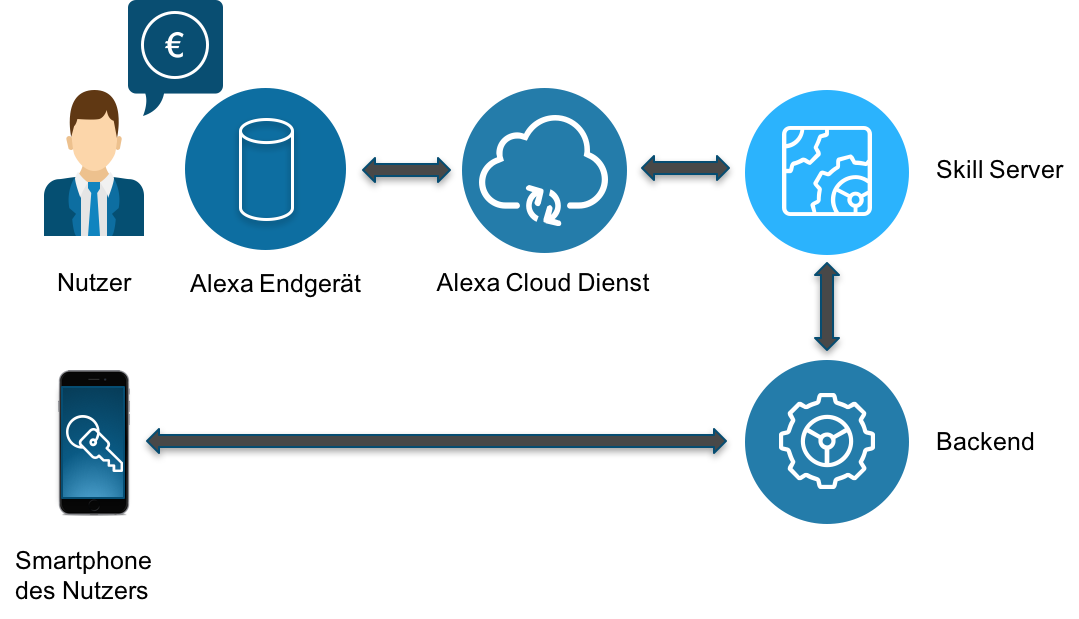
\includegraphics[width=1.0\textwidth]{bilder/3_securityConcept.png}
    \caption{Konzept für Authentifizierung}
    \label{fig:security-concept}
\end{figure}

Das Backend für die Registrierung ist bewusst als eigenständige Instanz und nicht als Teil des Skill-Servers konzipiert. Da dieser Mechanismus auch für andere \acp{VUI} Systeme (Cortana, Siri, \etc) funktionieren kann, ist man so unabhängig von der verwendeten Plattform.\\
Bevor ein Benutzer den Banking Skill verwenden kann, muss er sich zunächst über eine Smartphone App beim entsprechenden Server registrieren. Beim Starten oder bei Verwendung des Banking Skills, kann das System den Nutzer beispielsweise nach seinem Namen fragen. Im Anschluss wird geprüft, ob der Name bereits registriert ist. Daraufhin wird die Aufforderung zur Authentifizierung via \textit{Push Notification} an das Smartphone des Benutzers gesendet. Um den Gedanken aus der Umfrage aufzugreifen, ist hier eine Bestätigung per Fingerabdruck denkbar. Da der schnellere Zugang einer der Gründe für die Nutzung des Skills ist, stellt eine Fingerabdruck Abfrage einen guten Kompromiss zwischen Sicherheit und Effizienz dar. Erst wenn der Sprechende authentifiziert ist kann er alle Funktionen des Skill nutzen.\\
Alle Teilnehmer der Umfrage, der Interviews und User Tests haben große Sicherheitsbedenken. Auch wenn ein solcher Mechanismus Zeit kostet, wirkt sich dessen Verwendung möglicherweise positiv auf sicherheitskritische Nutzer aus. Es gibt noch einen Vorteil den dieses Konzept mit sich bringt. Die schützenswerten Daten für die Authentifzierung passieren dabei nicht die Amazon Plattform. Der Austausch findet abseits zwischen Smartphone-Anwendung und Backend statt. Die Informationen die an Alexa übertragen werden sind lediglich der Name des Benutzers und die Bestätigung, dass dieser authentifiziert ist.\\
Auch wenn die Stimmenerkennung für Alexa veröffentlicht wird, ist das hier beschriebene Konzept sinnvoll und kann als zusätzliche Maßnahme für mehr Sicherheit sorgen. Als Teil der Umsetzung in Kapitel \ref{cha:umsetzung} sind dort weitere Details dazu beschrieben.
\chapter{Umsetzung}
\label{cha:umsetzung}
Im Folgenden wird der \ac{HiFi}-Prototyp gemäß der Zielsetzung unter Kapitel \ref{sec:ziel-der-arbeit} umgesetzt. Die Umsetzung umfasst die dort konkret genannten Funktionen. Nutzern soll es möglich sein den Kontostand abzurufen und unter Verwendung von Vorlagen Überweisungen durchzuführen. Die Basis für die Implementierung bilden die dafür relevanten Ergebnisse aus der Konzeption unter Kapitel \ref{cha:konzeption}.\\
Die Implementierung jeder Komponente ist im jeweiligen Kapitel beschrieben. Dabei werden die verwendeten Technologien, Besonderheiten und Probleme erläutert. Da es in der Arbeit in erster Linie um die konzeptionellen Aspekte der Umsetzung geht, wird versucht auf die Darstellung von Quelltext zu verzichten. Sämtlicher Programmcode aller Komponenten ist auf der CD zu finden.\\
Vor der detaillierten Beschreibung der Umsetzung, wird an dieser Stelle noch der Name des Systems genannt. Dies ist kein zentraler Bestandteil der Arbeit, jedoch spielt er für das Starten des zu entwickelnden Alexa Skills (Invocation-Name) und auch für die Smartphone-App eine Rolle. Zunächst fällt die Wahl auf „finlexa“, eine Zusammensetzung aus „financial“ und „Alexa“. Das Problem dabei ist die Verwendung als Invocation-Name. Der Sprachbefehl zum Starten des Skills ist dann: 

\begin{center}
    „Alexa, starte finlexa“
\end{center}

Besser ist die zweite Wahl „Voice Bank“. Nicht nur der Sprachbefehl ist geeigneter, der Name sagt zudem aus, was die Anwendung bezweckt. Abbildung zeigt das dafür konstruierte Logo\footnote{Das Logo wurde von Isabella Thürauf entworfen.}.

\begin{figure}[h]
  \centering
  
\includegraphics[width=0.4\textwidth]{bilder/4_logo.png}
  \caption{Voice Bank Logo}
  \label{fig:voicebank-logo}
\end{figure}

\section{Vorüberlegungen}
\label{sec:umsetzung-vorueberlegung}
Als Voraussetzung für das Implementieren der Kontostand-Abfrage und der Transaktion via Vorlage, müssen weitere Stories aus \ref{sec:anhang-user-stories} umgesetzt werden. Das schließt nicht nur die Hilfe (1) und Eingabemöglichkeit der TAN (16) ein, welche als Teil des Skill-Servers agieren, auch die Folgenden gehören dazu:

\begin{itemize}
    \item \textbf{Profilverwaltung (2- 4) und Authentifizierung (5)}: Diese werden unter Verwendung des Sicherheits-Konzeptes aus Kapitel \ref{sec:sicherheits-konzept} umgesetzt. Dafür werden eine App und ein Backend entwickelt. Für das Speichern der Benutzerprofile ist dem Backend auch eine Datenbank anzubinden. Die App bildet das Frontend für deren Verwaltung. Außerdem können sich Nutzer für die Verwendung des Alexa Banking Skills über die App authentifizieren. 
    
    \item \textbf{Bankkonten-Anbindung (6- 9) und Wahl des Hauptkontos (9)}: Um den Kontostand abzufragen und Überweisungen durchzuführen müssen Benutzer ihre Konten zunächst an das System anbinden. Da das bereits genannte Sicherheits-Konzept ohnehin die Entwicklung einer App und eines Backends vorsieht, kann man diese auch für die Anbindung der Bankkonten nutzen. Ein registrierter und angemeldeter Benutzer soll seine Konten über die App mit dem System verbinden können. Dabei werden die für die Verwendung erforderlichen Informationen in der Datenbank gespeichert. Das Hauptkonto bestimmen die Nutzer ebenfalls über die App, indem eines der verknüpften Konten dafür ausgewählt wird. Da es sich hier um einen Prototypen handelt, werden die Bankkonten gemockt. Hierfür wird der in Kapitel \ref{sec:bankkonto-anbindung} beschriebene Dienst verwendet.
    
    \item \textbf{Verwaltung der Überweisungsvorlagen (10- 12)}: Ebenso wie die Konto-Anbindungen können Nutzer auch ihre Überweisungsvorlagen über die Smartphone-App verwalten. In der Datenbank werden die Vorlagen in Relation zum entsprechenden Benutzer gespeichert. 
\end{itemize}

Abbildung \ref{fig:umsetzung-komponenten} zeigt eine Komponentenübersicht, in der diese Überlegungen einfließen.\newpage

\begin{figure}[!htb]
    \centering
    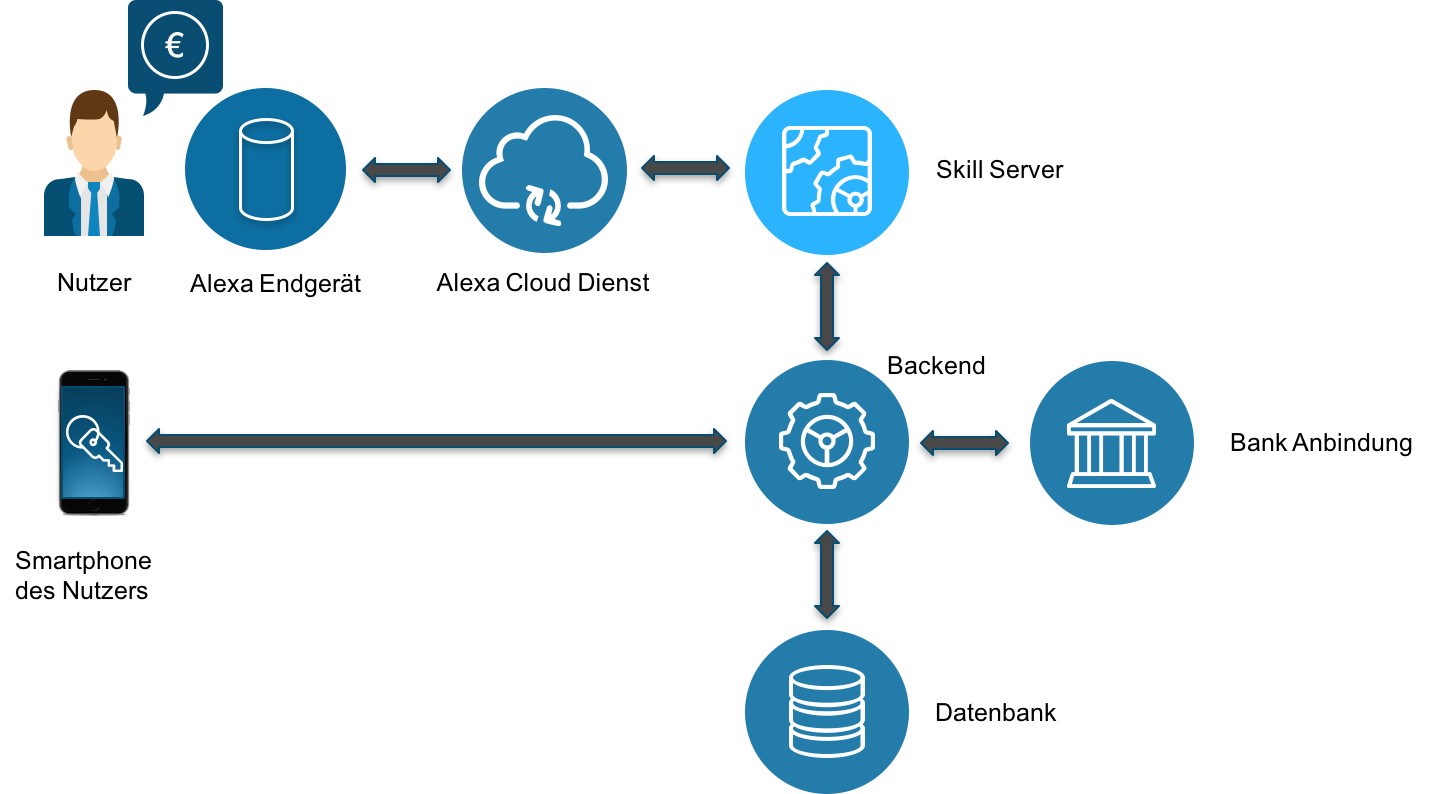
\includegraphics[width=1.0\textwidth]{bilder/4_umsetzungKomponenten.png}
    \caption{Komponentenübersicht für die Umsetzung}
    \label{fig:umsetzung-komponenten}
\end{figure}

Wie bereits erwähnt, speichert die Datenbank Benutzerprofile, Überweisungs-Vorlagen und Bankkonten-Anbindungen. Zunächst werden die dafür benötigten Datenmodelle beschrieben. Abbildung \ref{fig:datenbank-modell} zeigt eine vereinfachte Darstellung.

\begin{figure}[!htb]
    \centering
    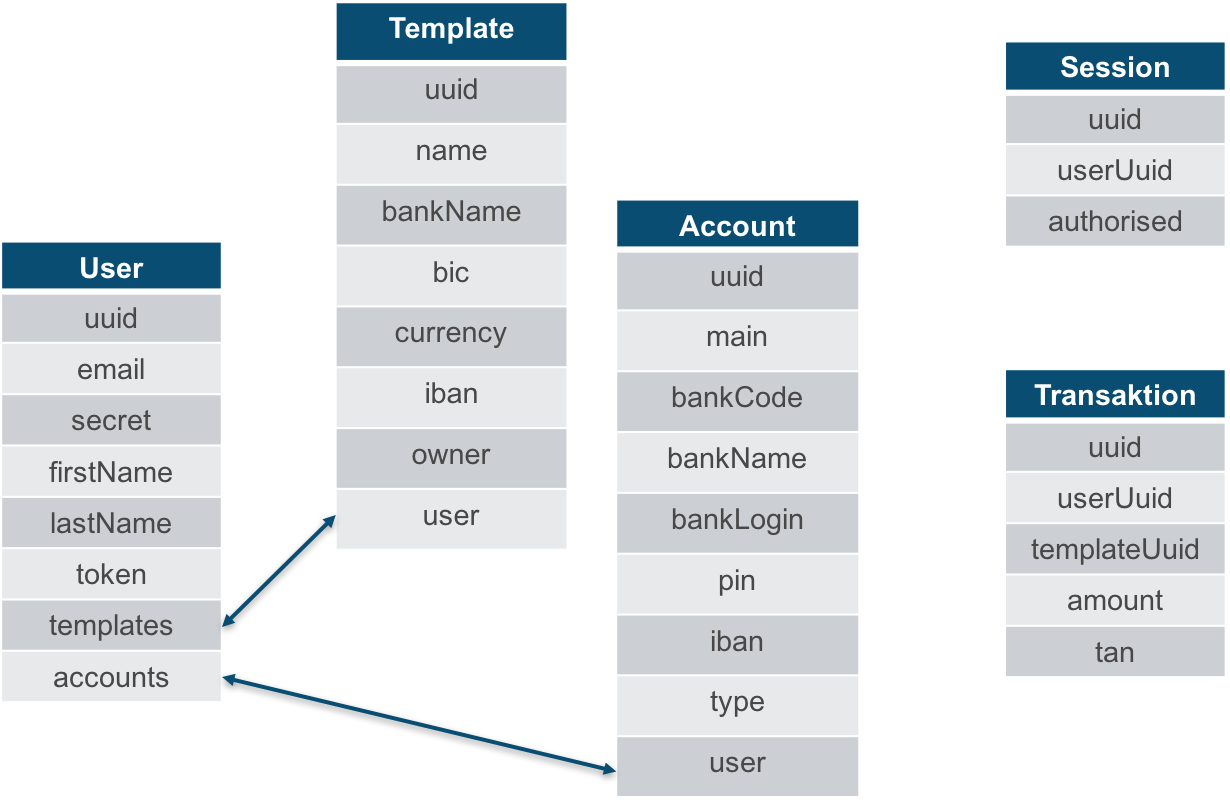
\includegraphics[width=0.8\textwidth]{bilder/4_datenmodelle.png}
    \caption{Vereinfachte Darstellung der Objekte und Relationen für die Datenbank}
    \label{fig:datenbank-modell}
\end{figure}

Jedes der Modelle hat einen \textit{\ac{UUID}}, um die Datensätze eindeutig zu kennzeichnen. Für ein Benutzerprofil sind nicht nur die Anmeldedaten wichtig, wie hier die Email Adresse und das Passwort (Secret). Der Vorname wird benötigt, um die Authentifizierung via Alexa für diesen anzustoßen. Für den Fall, dass Benutzer den gleichen Vornamen haben dient der Nachname der Unterscheidung dieser Nutzer. Mit Hilfe des Tokens wird das Smartphone des hinterlegten Benutzers für die Push-Nachrichten adressiert. Diese werden in den Kapiteln \ref{sec:backend} und \ref{sec:app} genauer betrachtet. Außerdem gehören Templates und Accounts zum Benutzerprofil, welche mit den entsprechenden Datensätzen verknüpft sind. Dabei handelt es sich um die Überweisungs-Vorlagen und Bankkonten-Anbindungen, die dieser Nutzer angelegt hat. Eine Überweisungs-Vorlage enthält alle notwendigen Informationen für das Durchführen von Transaktionen über Alexa, darunter die Zielbank, \ac{BIC}, \ac{IBAN} des Zielkontos und der Kontoinhaber. Beim Anlegen der Vorlage muss der Benutzer einen Namen vergeben, um die Vorlage über Alexa zu adressieren. Der Betrag ist nicht Bestandteil der Vorlage, da dieser vom Benutzer über Sprache eingegeben wird.\\ 
Die Konto-Anbindung speichert ebenfalls die Daten für den Login, die für die Anmeldung bei der entsprechenden Online-Banking-Anwendung verwendet werden. Neben der \ac{IBAN} wird auch der Typ des Kontos gespeichert. Dieser kann vom Nutzer festgelegt werden und dient als Orientierungshilfe in der App. Das Feld „main“ sagt aus, ob es sich bei diesem Konto um das Hauptkonto handelt. Auch die Konto-Anbindung verweist auf den Benutzer, der die Verknüpfung angelegt hat.\\
Die Datenbank wird entsprechend dieser Modelle an das Backend angebunden. Das heißt, dass nur das Backend einen direkten Zugriff auf diese Daten hat. Damit auch andere Anwendungen auf die Daten zurückgreifen können, muss das Backend eine Schnittstelle zur Verfügung stellen, die von diesen Anwendungen konsumiert werden kann. Diese Schnittstelle wird zunächst modelliert.\\
Es gibt verschiedene Formen der Interoperabilität zwischen Diensten im Internet. Eine dieser Formen ist \ac{REST}. Da die Alexa Plattform mit dem Skill-Server via \ac{REST} kommuniziert, soll auch das Backend eine solche Schnittstelle bereit stellen. Tabelle \ref{tab:backend-rest-api} zeigt die modellierte \ac{REST}-Schnittstelle. Dabei werden die \textit{\ac{CRUD}} Operationen für Profile, Bank-Anbindungen und Überweisungs-Vorlagen umgesetzt. \ac{CRUD} definiert die vier Basis Operationen für persistenten Speicher. Einige der Endpunkte beinhalten geklammerte Ausdrücke, wie \zB „\{userId\}“. Diese stellen Parameter dar, die sich für jede Anfrage ändern können. Alle Id-Parameter sind Platzhalter für die \ac{UUID} des jeweiligen Datensatzes. 

\begin{table}[!h]
\centering
 \begin{tabular}{ | m{4.5cm} || C{2cm}| C{2cm} | C{2cm} | C{2cm} |} 
 \hline
 Ressource & POST & GET & PUT & DELETE\\ 
 Endpunkt & create & read & update & delete \\
 \hhline{=::====}
  /users & Profil anlegen & Alle Profile ausgeben & n.a. & n.a.\\ 
 \hline /users/\{userId\} & n.a. & Profil ausgeben & Profil bearbeiten & Profil löschen\\
 \hline /users/\{userId\}/accounts & Account anlegen & Alle Accounts des Nutzers ausgeben & n.a. & n.a.\\
 \hline /users/\{userId\}/accounts/\{accId\} & n.a. & Account ausgeben & Account bearbeiten & Account löschen\\
 \hline /users/\{userId\}/templates & Template anlegen & Alle Templates des Nutzers ausgeben & n.a. & n.a.\\ 
 \hline /users/\{userId\}/templates/
 \{tmpId\} & n.a. & Template ausgeben & Template bearbeiten & Template löschen\\ 
 \hline
\end{tabular}
\caption{Backend REST-Schnittstelle für die Verwaltung von Profilen, Bank-Anbindungen und Überweisung-Vorlagen}
\label{tab:backend-rest-api}
\end{table}

Die hier modellierte \ac{REST}-Schnittstelle für das Backend setzt in Verbindung mit der App die Stories für die Verwaltung von Profilen (2-4), Bank-Anbindungen (6-9) und Überweisungs-Vorlagen (10-12) um. Für die eigentlichen Banking Funktionalitäten über Alexa, darunter die Authentifizierung (5), Kontostand Abfrage (13), Transaktion (14) und TAN-Eingabe (16), muss der Skill-Server mit dem Backend kommunizieren. Auch für diese Kommunikation soll das Backend eine \ac{REST}-Schnittstelle definieren. Zunächst wird der Vorgang der Authentifizierung näher betrachtet. \\
Benötigt man für die Verwendung eines Alexa Skills zusätzliche Endgeräte, wie hier das Smartphone, sind gewisse Dinge zu beachten. Alexa funktioniert nach dem Frage-Antwort-Prinzip. Ein Benutzer stößt die Interaktion an und der Skill-Server gibt die Antwort zurück. Alexa kann dabei nicht über Ereignisse (engl. Events) gesteuert werden. Gemäß Kapitel \ref{sec:sicherheits-konzept} startet die Authentifizierung, sobald der Name des Benutzers eingegeben wird. Nun kann zwar die Aufforderung an das Smartphone des Nutzers gesendet werden, jedoch kann die Bestätigung des Fingerabdrucks nicht direkt die Ausgabe über Alexa anstoßen. Aus diesem Grund werden Session-Objekte verwendet. Sie werden vom Backend verwaltet und ebenfalls in der Datenbank gespeichert. Abbildung \ref{fig:datenbank-modell} zeigt auch das Modell der Session. Nennt ein Benutzer seinen Namen wird ein Session-Objekt im Backend \bzw der Datenbank angelegt und die Aufforderung zur Bestätigung des Fingerabdruckes an das mobile Endgerät geschickt. Für einen besseren Überblick wird im Folgenden das Zusammenspiel zwischen Skill-Server, Backend und App für den Authentifizierungsprozess dargestellt. Abbildung \ref{fig:sequenz-authentifizierung} zeigt diesen in Form eines Sequenzdiagrammes. 

\begin{figure}[!htb]
    \centering
    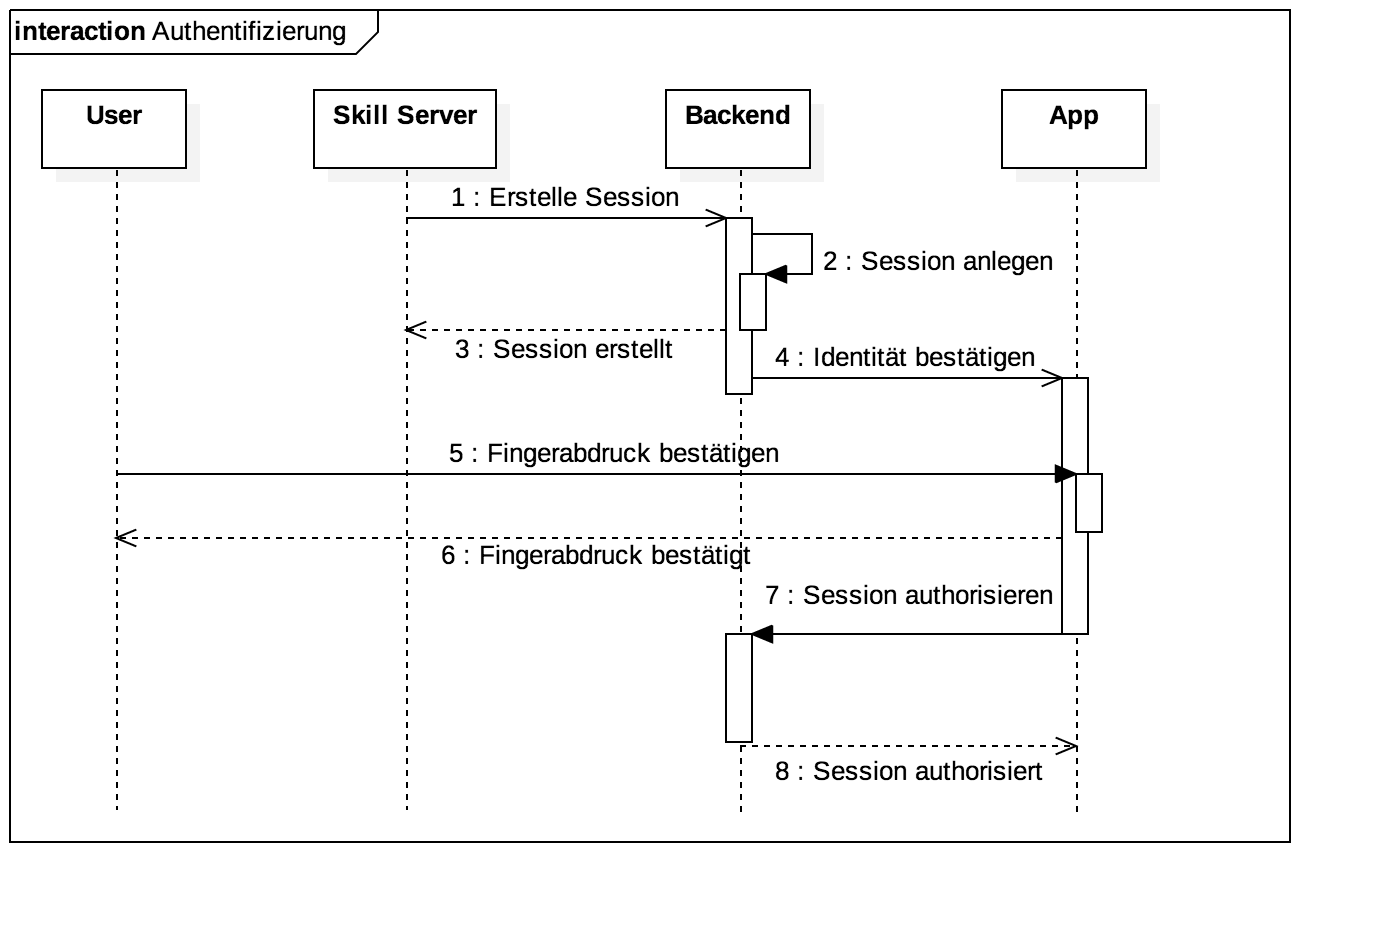
\includegraphics[width=1.0\textwidth]{bilder/4_sequenzAuthentifizierung.png}
    \caption{Sequenzdiagramm für den Authentifizierungsprozess}
    \label{fig:sequenz-authentifizierung}
\end{figure}

Bei erfolgreicher Authentifizierung teilt nun die App dem Backend mit, dass diese Session autorisiert ist. Im Anschluss können die Banking Funktionen über Alexa genutzt werden. Wird der Skill beendet ist die Authorisierung nichtig. Bei erneutem Öffnen muss der Vorgang wiederholt werden. Im Folgenden wird der Prozess der Kontostand-Abfrage betrachtet.\\
Ist die Session des Benutzers autorisiert, kann der Kontostand abgefragt werden. Da das Backend als Vermittler zwischen Skill-Server und Bank-Anbindung agiert (\vgl Abbildung \ref{fig:umsetzung-komponenten}), wird auch hierfür ein Endpunkt benötigt, der vom Skill-Server angesprochen werden kann. Bei Verwendung holt sich das Backend, über das vom Benutzer hinterlegte Hauptkonto die Information von der Bank-Anbindung. Abbildung \ref{fig:sequenz-kontostand} veranschaulicht den Prozess.\newpage

\begin{figure}[!htb]
    \centering
    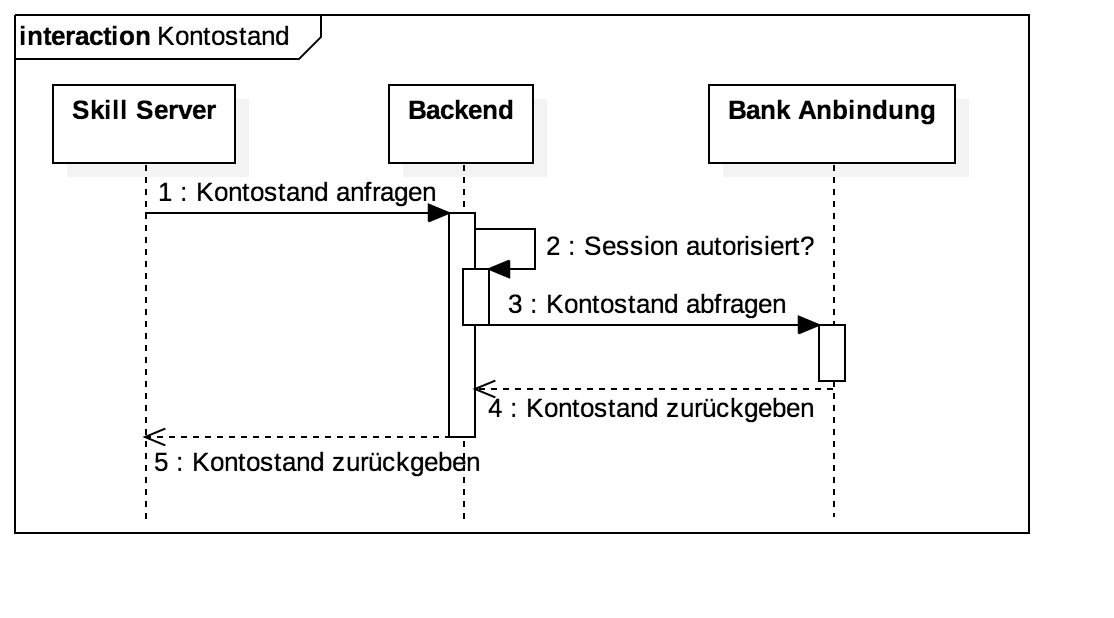
\includegraphics[width=1.0\textwidth]{bilder/4_sequenzKontostand.png}
    \caption{Sequenzdiagramm für die Abfrage des Kontostandes}
    \label{fig:sequenz-kontostand}
\end{figure}

Die Durchführung einer Transaktion ist ähnlich. Der Skill-Server sendet eine Anfrage mit den für die Überweisung benötigten Daten an das Backend. Anders als die Kontostand Abfrage muss eine Transaktion zusätzlich über die Eingabe einer \ac{TAN} bestätigt werden. Auch hier kann vorerst ein Objekt angelegt werden, welches sämtliche Informationen für die Durchführung der Überweisung enthält (\vgl Abbildung \ref{fig:datenbank-modell}). Darunter der Benutzer und die verwendete Überweisungsvorlage in Form der entsprechenden \acp{UUID}. Zusätzlich wird der Betrag für die Durchführung benötigt. Da es sich um einen Prototypen handelt und die Bankkonten gemockt werden, gibt es keine Bank für die Generierung der \ac{TAN}. Sie muss vom Backend erzeugt werden. Dieser Prozess wird in Abbildung \ref{fig:sequenz-transaktion-anlegen} veranschaulicht.\newpage

\begin{figure}[!htb]
    \centering
    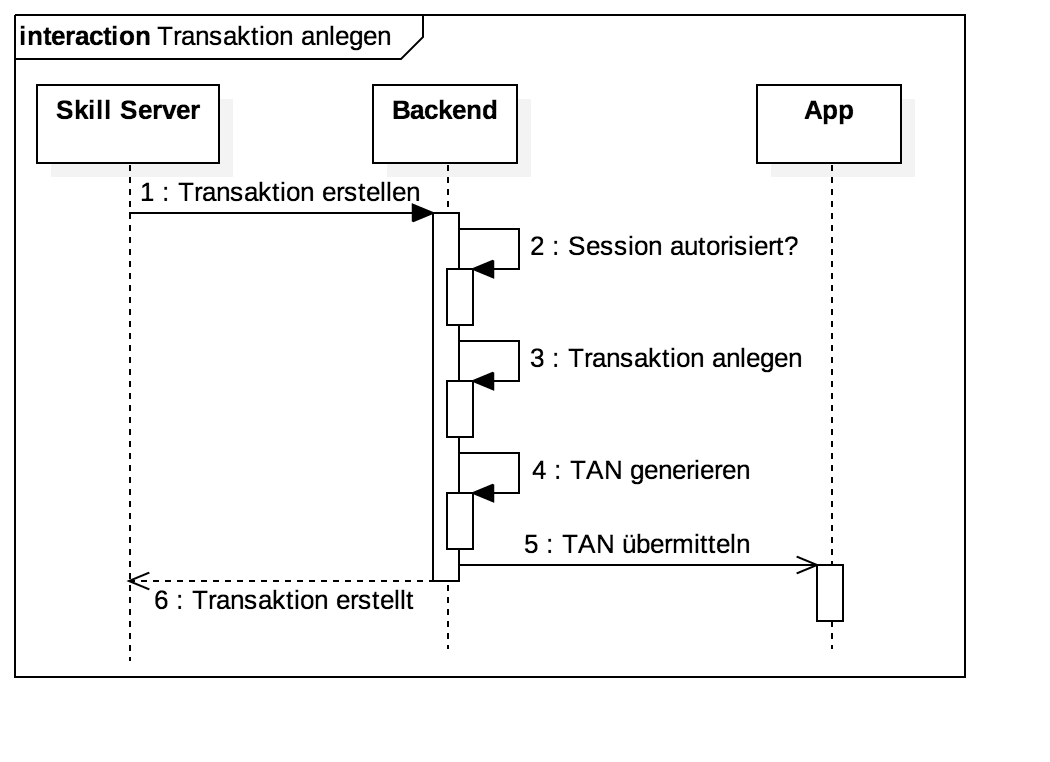
\includegraphics[width=1.0\textwidth]{bilder/4_sequenzTransaktionAnlegen.png}
    \caption{Sequenzdiagramm für das Anlegen einer Transaktion}
    \label{fig:sequenz-transaktion-anlegen}
\end{figure}

Im Anschluss wird dem Benutzer die Nummer per Smartphone-App übermittelt. Nachdem er die \ac{TAN} in den Echo diktiert hat wird diese validiert. Ist die Nummer korrekt wird die Transaktion bestätigt und an die Bank-Anbindung gesendet, zu sehen in Abbildung \ref{fig:sequenz-transaktion-bestaetigen}.\newpage 

\begin{figure}[!htb]
    \centering
    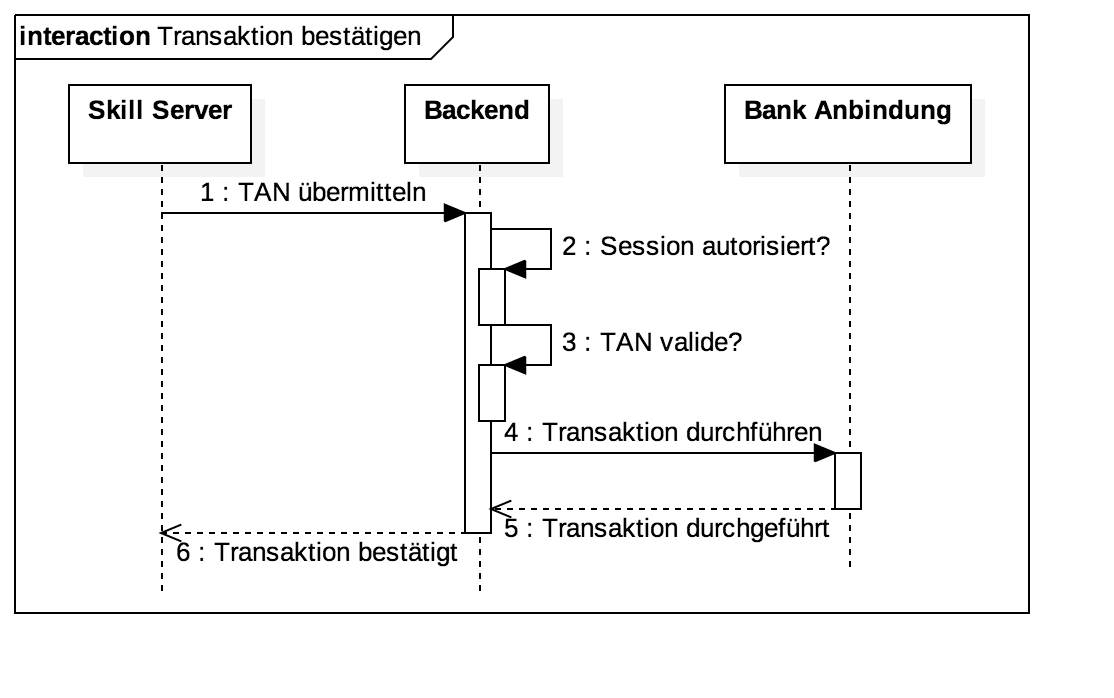
\includegraphics[width=1.0\textwidth]{bilder/4_sequenzTransaktionbestaetigen.png}
    \caption{Sequenzdiagramm für das Bestätigen einer Transaktion}
    \label{fig:sequenz-transaktion-bestaetigen}
\end{figure}

Das Diktieren der \ac{TAN} über den Echo ist dabei unkritisch, da diese Nummer nur einmal gültig ist.\\
Zusätzlich zur bereits gezeigten Schnittstelle benötigt das Backend also eine weitere für die Ausführung der beschriebenen Banking-Funktionen. Daraus ergibt sich das in Tabelle \ref{tab:backend-banking-rest-api} gezeigte Modell.

\begin{table}[!htb]
\centering
 \begin{tabular}{ | m{4cm} || C{2cm}| C{2cm} | C{2cm} | C{2cm} |} 
 \hline
 Ressource & POST & GET & PUT & DELETE\\ 
 Endpunkt & create & read & update & delete\\
 \hhline{=::====}
  /sessions & Session anlegen & Alle Sessions ausgeben & n.a. & n.a.\\ 
 \hline /sessions/\{sessionId\} & Session authorisieren & Session ausgeben & Autorisierung erneut senden & n.a.\\
 \hline /balance & Kontostand ausgeben & n.a. & n.a. & n.a.\\
\hline/transactions & Transaktion anlegen & Alle Transaktionen ausgeben & n.a. & n.a.\\ 
 \hline /transactions/\{transId\} & n.a. & Transaktion ausgeben & n.a. & n.a.\\ 
\hline /transactions/\{transId\}/\{tan\} & Transaktion bestätigen & n.a. & n.a. & n.a.\\ 
 \hline
\end{tabular}
\caption{Backend REST-Schnittstelle für Banking Funktionen}
\label{tab:backend-banking-rest-api}
\end{table}

Die folgenden Kapitel beschreiben die Implementierung jeder Komponente aus Abbildung \ref{fig:umsetzung-komponenten}. Der Fokus der Arbeit liegt auf der Umsetzung des \ac{CUI}. Aus diesem Grund werden die Kapitel des Skill-Servers (\ref{sec:skill-server}) und Interaction Models (\ref{sec:interaction-model}) detaillierter beschrieben. Für die anderen Kapitel soll lediglich ein Überblick gegeben werden. 

\section{Bank-Anbindung}
\label{sec:bankkonto-anbindung}
Da es sich bei der Umsetzung um einen Prototypen handelt, werden keine realen Konten an das System angebunden. Die Daten werden über den \textit{Multibanking-Mock-Service} simuliert. Dabei handelt es sich um einen bereits existierenden Dienst, der vom Projektträger der Arbeit bereit gestellt wird. Im weiteren Verlauf wird dieser als Multibank-Mock oder einfach nur Mock bezeichnet. Neben diesem gibt es auch den \textit{Multibanking-Service}. Darüber ist die Anbindung realer Konten möglich. Da die Datenmodelle beider Services ähnlich sind, ist eine spätere Integration des Multibanking-Service gut umzusetzen. Der Mock wird beim Projektträger verwendet, um entwickelte Anwendungen mit Kontodaten zu testen. Die Konten kann man dabei beliebig konfigurieren. Kontostände, Buchungen, Daueraufträge \usw können über die \ac{REST}-Schnittstelle des Mocks \bzw dem Hochladen einer Excel-Tabelle bequem eingerichtet und geändert werden. Da der Fokus der Arbeit ein anderer ist, werden hier Datenmodell und Endpunkte des Mocks nicht näher erläutert. Für den späteren Test des Prototypen wird mit dessen Hilfe ein Konto erstellt und an das System angebunden.

\section{Backend}
\label{sec:backend}
Das Backend ist die vermittelnde Instanz zwischen Skill-Server, Smartphone-App, Datenbank und Bank-Anbindung. Ein Teil der Funktionalität ist bereits in Kapitel \ref{sec:umsetzung-vorueberlegung} konzeptionell beschrieben. Die dort beschriebenen \ac{REST}-Schnittstellen und die Datenbank-Anbindung werden im Backend umgesetzt. Die Prozesse der Authentifizierung sehen außerdem vor, dass das Backend Informationen an die Smartphone-App übermittelt. Wie in Kapitel \ref{sec:sicherheits-konzept} erwähnt, soll dies über Push-Nachrichten erfolgen, daher ist auch diese Funktionalität im Backend zu implementieren. 

\subsection{Datenbank}
\label{subsec:backend-datenbank}
Als Datenbank aus Abbildung \ref{fig:umsetzung-komponenten} kommt \textit{PostgreSQL} \cite{postgres} zum Einsatz. Dabei handelt es sich um eine Open-Source \textit{\ac{SQL}} Datenbank. Für diese Wahl gibt es keinen bestimmten Grund.

\subsection{Plattform}
\label{backend-plattform}
Bei der Implementierung des Backends wird \textit{Node.js} \cite{node-js} verwendet, eine serverseitige \textit{\ac{JS}} Plattform. Da bei der Alexa Skill Entwicklung größtenteils darauf zurückgegriffen wird, ist der Skill-Server ebenfalls in Node.js entwickelt. Im Bereich des Backends gibt es jedoch keinen speziellen Grund dafür. Eine Node.js Anwendung kann über den \textit{\ac{npm}} \cite{npm}, mit zusätzlichen Open-Source Bibliotheken, sogenannten Modulen, erweitert werden. Auf die wichtigsten Bibliotheken wird im Folgenden eingegangen.

\begin{itemize}
    \item \textit{Express}: Express ist ein minimalistisches und flexibles Node.js Framework für Web-Anwendungen, dass vieles an Funktionalität mit sich bringt. Hier wird es in erster Linie für den Aufbau der Endpunkte, der Integration von \textit{Middleware}\footnote{Bei Web Servern handelt es sich dabei um Routinen, die zwischen dem Endpunkt und der eigentlichen Businesslogik greifen.} und dem Starten der Backend-Anwendung verwendet. Express erleichtert vor allem die Umsetzung der in Kapitel \ref{sec:umsetzung-vorueberlegung} beschriebenen \ac{REST}-Schnittstellen \cite{express-js}.
    
    \item \textit{\ac{TS}}: TypeScript ist ein typisiertes Superset von \ac{JS}. Es ermöglicht die Implementierung von Klassen und ist typensicher, was die ausschlaggebenden Gründe für die Verwendung sind. Der Quelltext des Backends und des Skill-Servers sind in \ac{TS} geschrieben. Für die Ausführung des Programmcodes wird der Quelltext vorher in \ac{JS} kompiliert \cite{typescript}. 
    
    \item \textit{TypeORM}: Dabei handelt es sich um ein Modul für \textit{\ac{ORM}}. Diese Technik wird im Allgemeinen dafür verwendet, Daten zwischen System mit inkompatiblen Typen zu transferieren. Im Backend wird \ac{ORM} für die Datenbank-Anbindung genutzt. Es erlaubt eine komfortable Verwaltung der Daten unter Verwendung bereits implementierter \ac{TS} Typen \bzw Klassen. Das Schreiben von \textit{\ac{SQL}} Methoden entfällt dabei \cite{typeorm}.
    
    \item \textit{Firebase}: Firebase ist eine freie Plattform, die bei der Entwicklung von mobilen Anwendungen unterstützt. Sie bietet dabei viele unterschiedliche Funktionen an. Hier wird lediglich das \textit{Cloud Messaging} verwendet, um die Push-Nachrichten für die Authentifizierung und das Versenden der \ac{TAN} umzusetzen. Um Firebase nutzen zu können, muss man sich zunächst registrieren und seine Anwendung hinterlegen. Das Backend agiert als der Server, der die Nachrichten über Firebase an die hinterlegte App schickt. Dafür ist im Backend die „Firebase Service“ Klasse implementiert. Für Nutzung des Dienstes, werden Daten aus dem Firebase Benutzerprofil benötigt. Um diese Daten bei Veröffentlichung der Arbeit zu schützen, wird der Teil des Quelltextes entfernt und entsprechend kommentiert \cite{firebase}.
\end{itemize}

Der Programmcode des Backends ist auf der beiliegenden CD unter \textit{„Quelltexte/finlexa\_central/“} zu finden.

\section{Smartphone Anwendung}
\label{sec:app}
Die App ist nicht nur ein wichtiger Teil des Sicherheits-Konzeptes, sondern bildet auch das Frontend für die Verwaltung der Profile, Überweisungsvorlagen und Bankkonten-Anbindungen. Auch hier soll nur ein Überblick gegeben und nicht im Detail auf den Quelltext eingegangen werden. Die App ist für das \textit{Android} Betriebssystem \cite{android} implementiert. Im Folgenden werden anhand der erstellten Oberflächen die grundlegenden Funktionen der Anwendung erklärt. Aufgrund der zeitlichen Begrenzung beschränkt sich die Anwendung in erster Linie auf die Funktionalität. Gestaltung und Usability liegt hier nicht im Fokus.

\subsection{Registrieren und anmelden}
\label{subsec:app-registrieren-anmelden}
Damit sich Benutzer registrieren können, wird die entsprechende \ac{REST}-Schnittstelle des Backends konsumiert. Abbildung \ref{fig:app-login} zeigt die Bildschirme für den Login-Bereich und der Registrierung. Letzterer wird durch Klicken des Buttons auf dem Login-Bildschirm geöffnet.

\begin{figure}[h]
  \centering
  \begin{minipage}[b]{0.45\textwidth}
    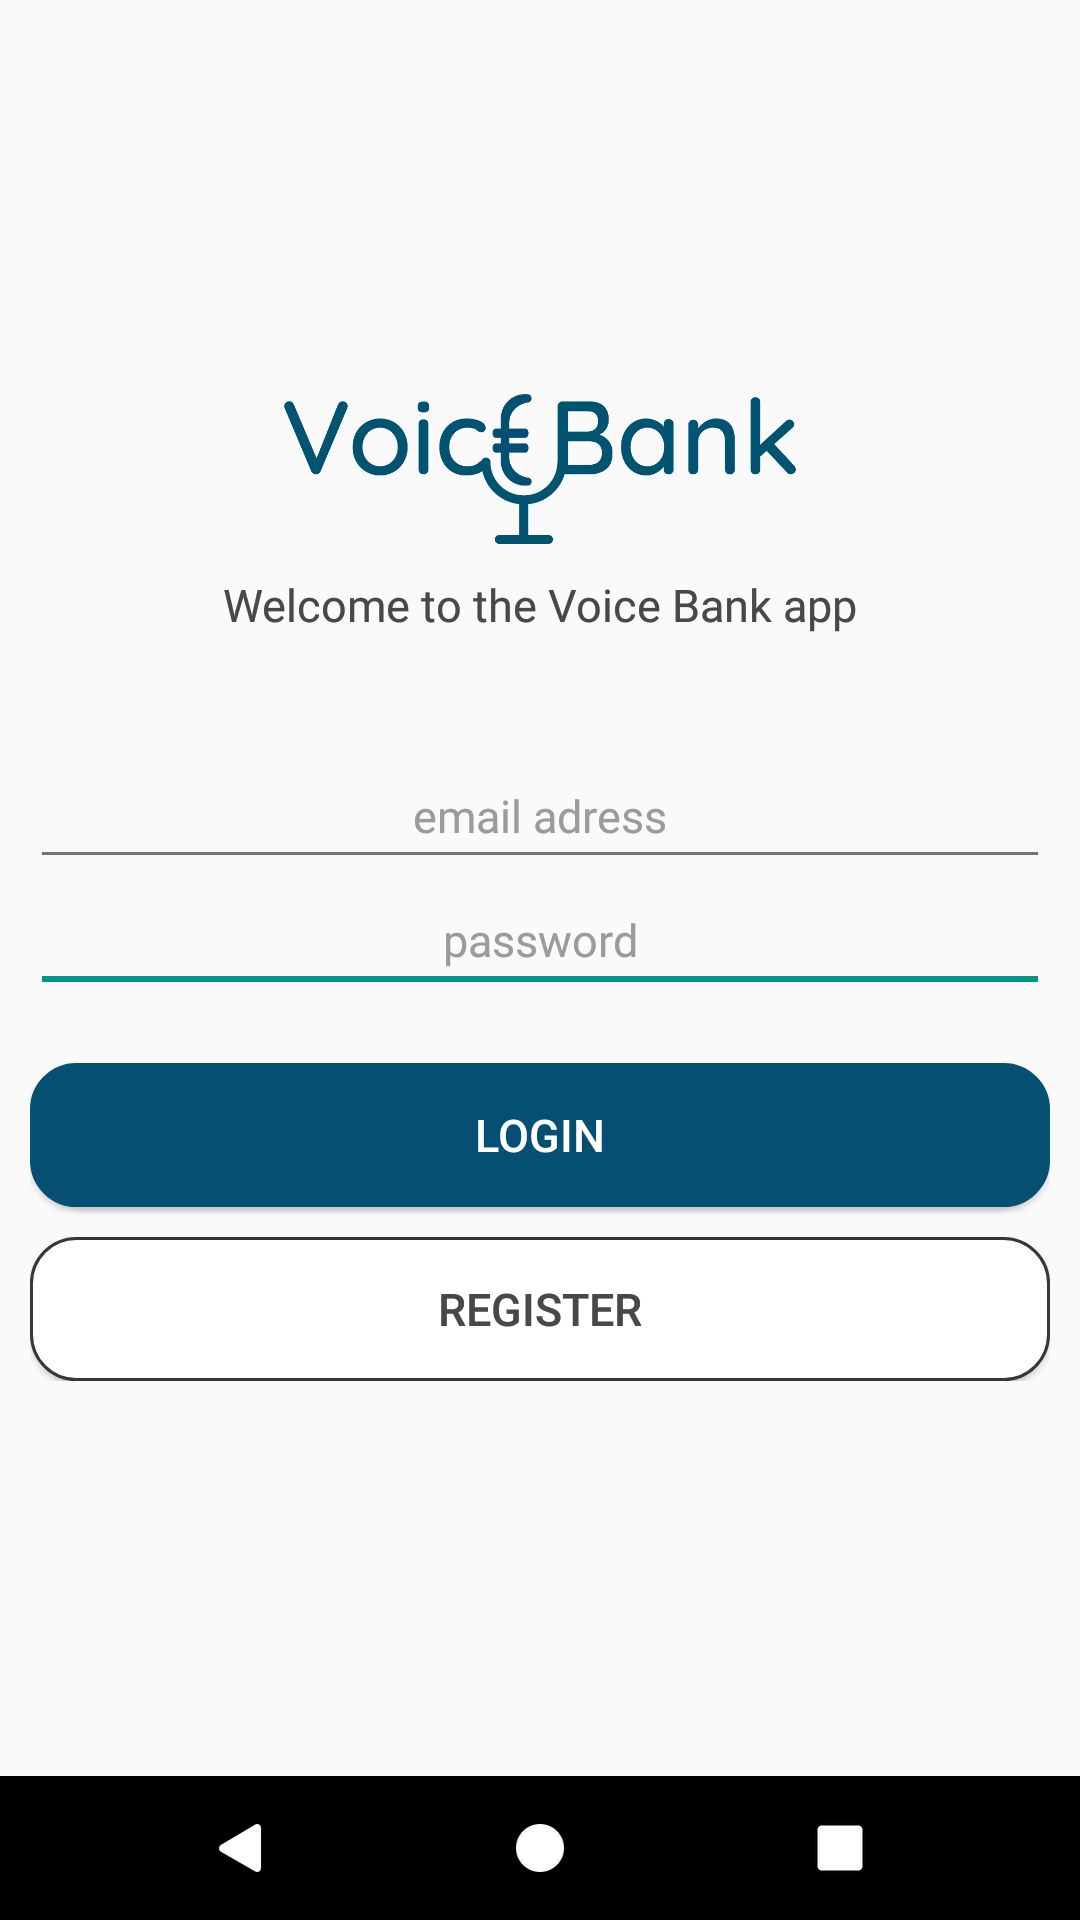
\includegraphics[width=\textwidth]{bilder/4_appLogin.png}
  \end{minipage}
  \begin{minipage}[b]{0.45\textwidth}
    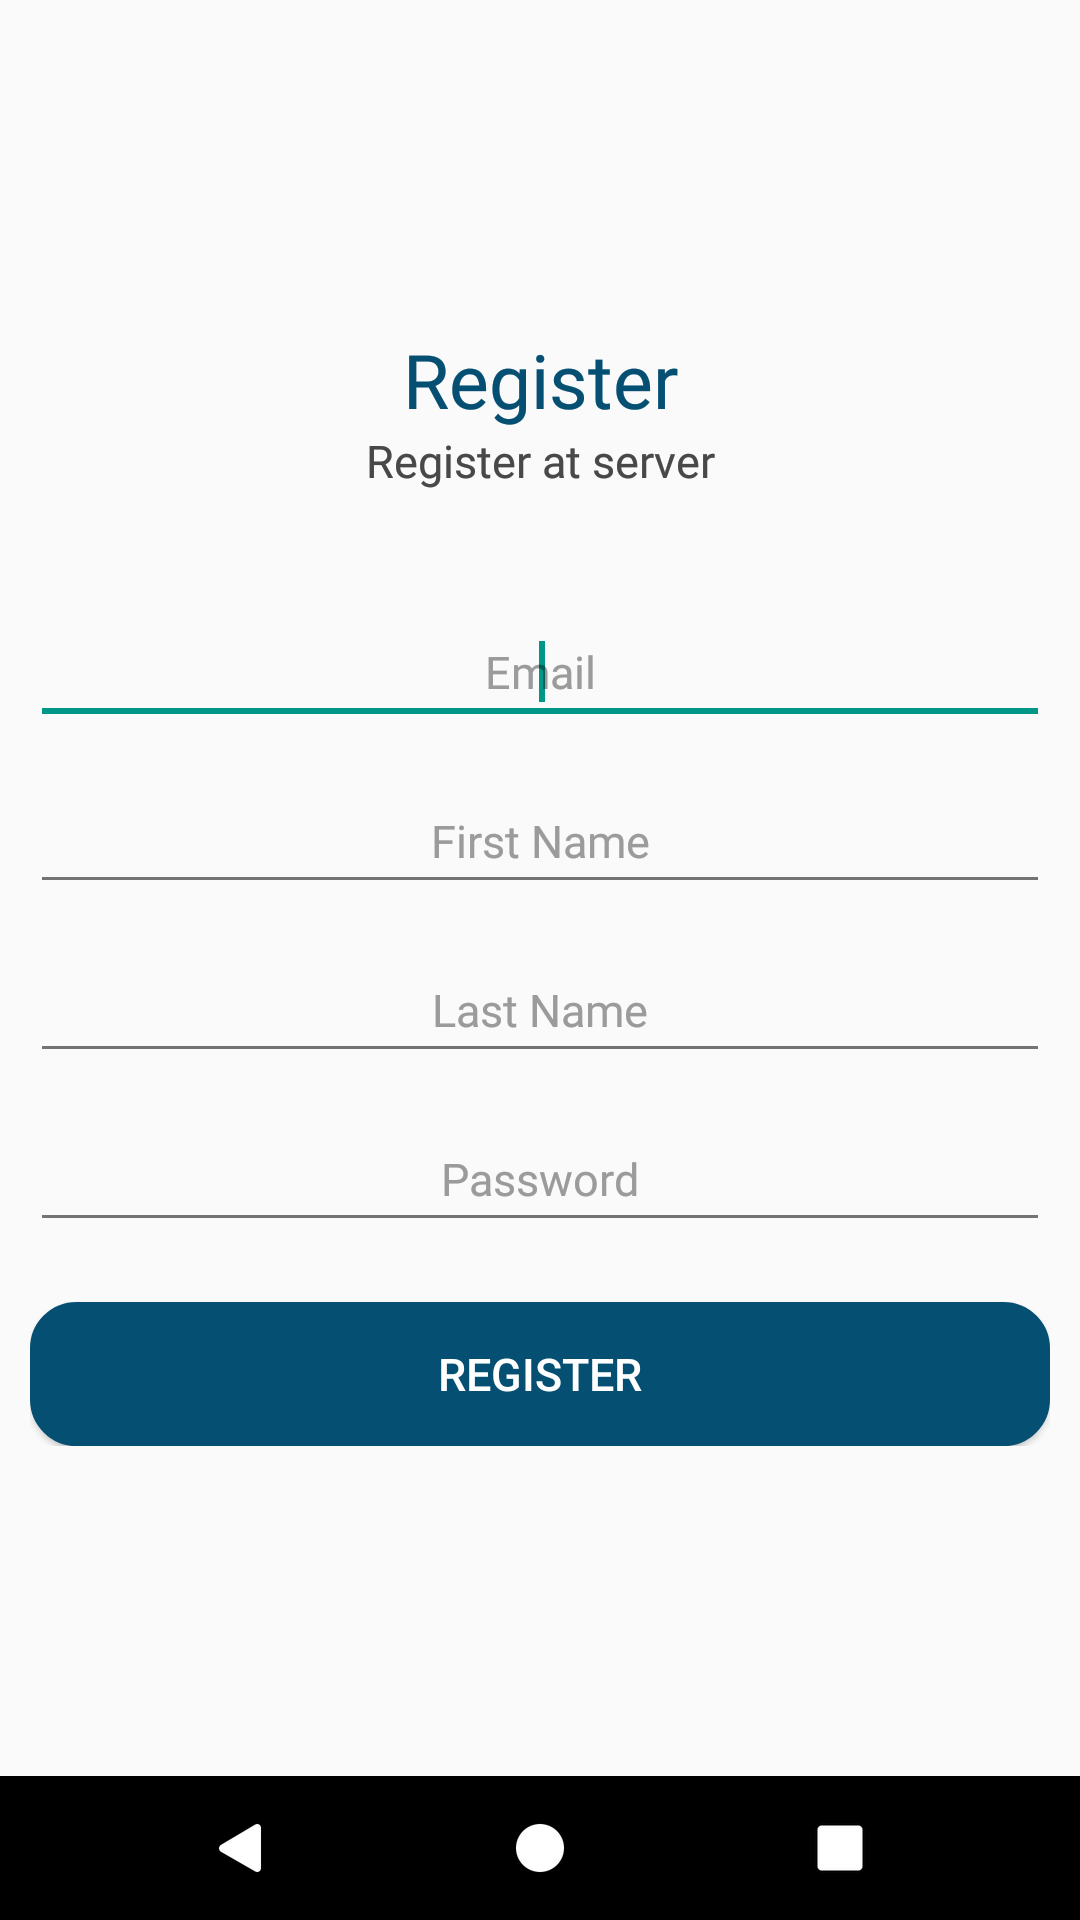
\includegraphics[width=\textwidth]{bilder/4_appRegister.png}
  \end{minipage}
  \caption{Login- und Registrierungs-Bildschirm der Voice Bank App}
  \label{fig:app-login}
\end{figure}

Hat sich ein Benutzer registriert, kann er sich unter Eingabe der Daten anmelden. Im Anschluss kann man Überweisungs-Vorlagen und die Anbindungen der Bankkonten verwalten. Für die App wird ebenfalls Firebase implementiert, um die vom Backend generierten Push-Nachrichten zu empfangen. Beim Registrieren eines Benutzers wird der Firebase Token in der Datenbank hinterlegt (\vgl Abbildung \ref{fig:datenbank-modell}). Dieser Token adressiert die Voice Bank App eines Benutzers für die Push-Nachrichten des Backends.

\subsection{Verwalten}
\label{subsec:app-verwalten}
Nachdem sich ein Benutzer angemeldet hat, erscheinen die Oberflächen für die Verwaltung der Vorlagen und Anbindungen. Abbildung \ref{fig:app-accounts} zeigt links die Liste der angebundenen Konten.

\begin{figure}[h]
  \centering
  \begin{minipage}[b]{0.45\textwidth}
    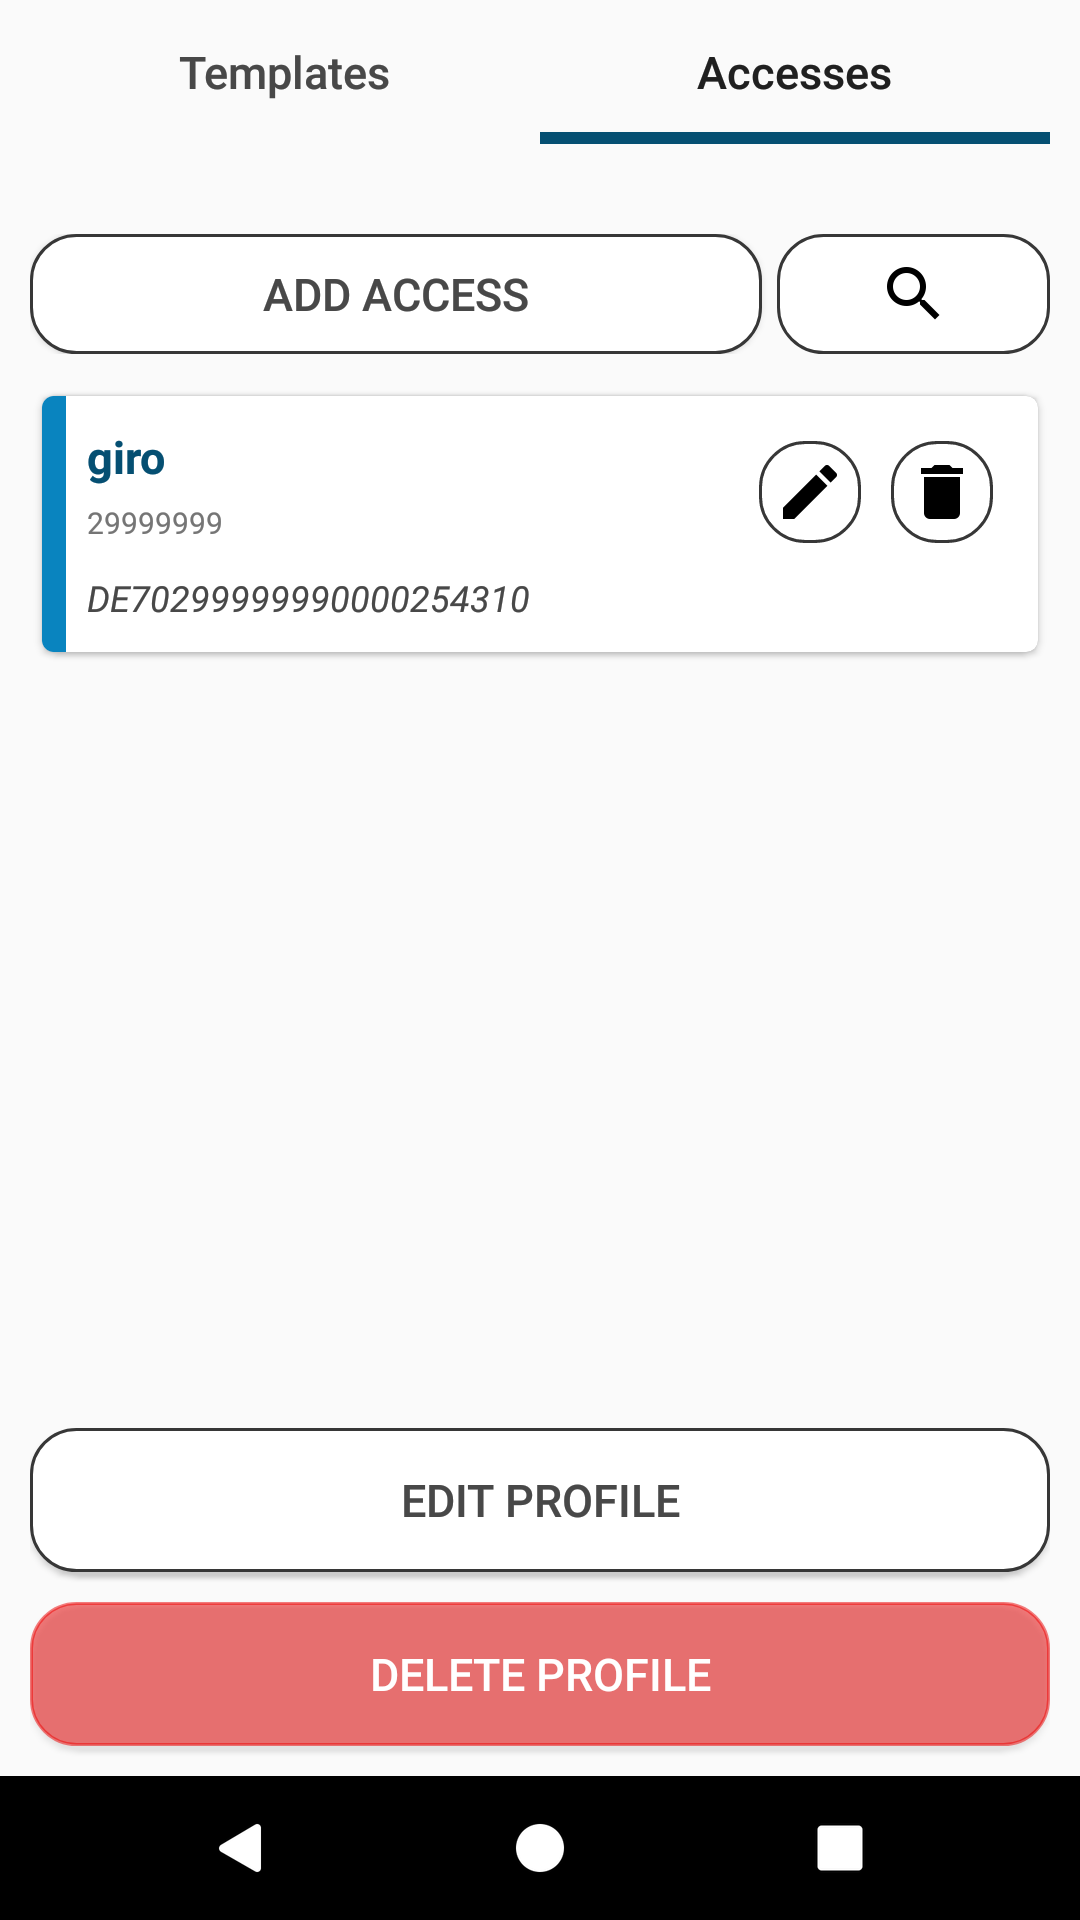
\includegraphics[width=\textwidth]{bilder/4_appAccounts.png}
  \end{minipage}
  \begin{minipage}[b]{0.45\textwidth}
    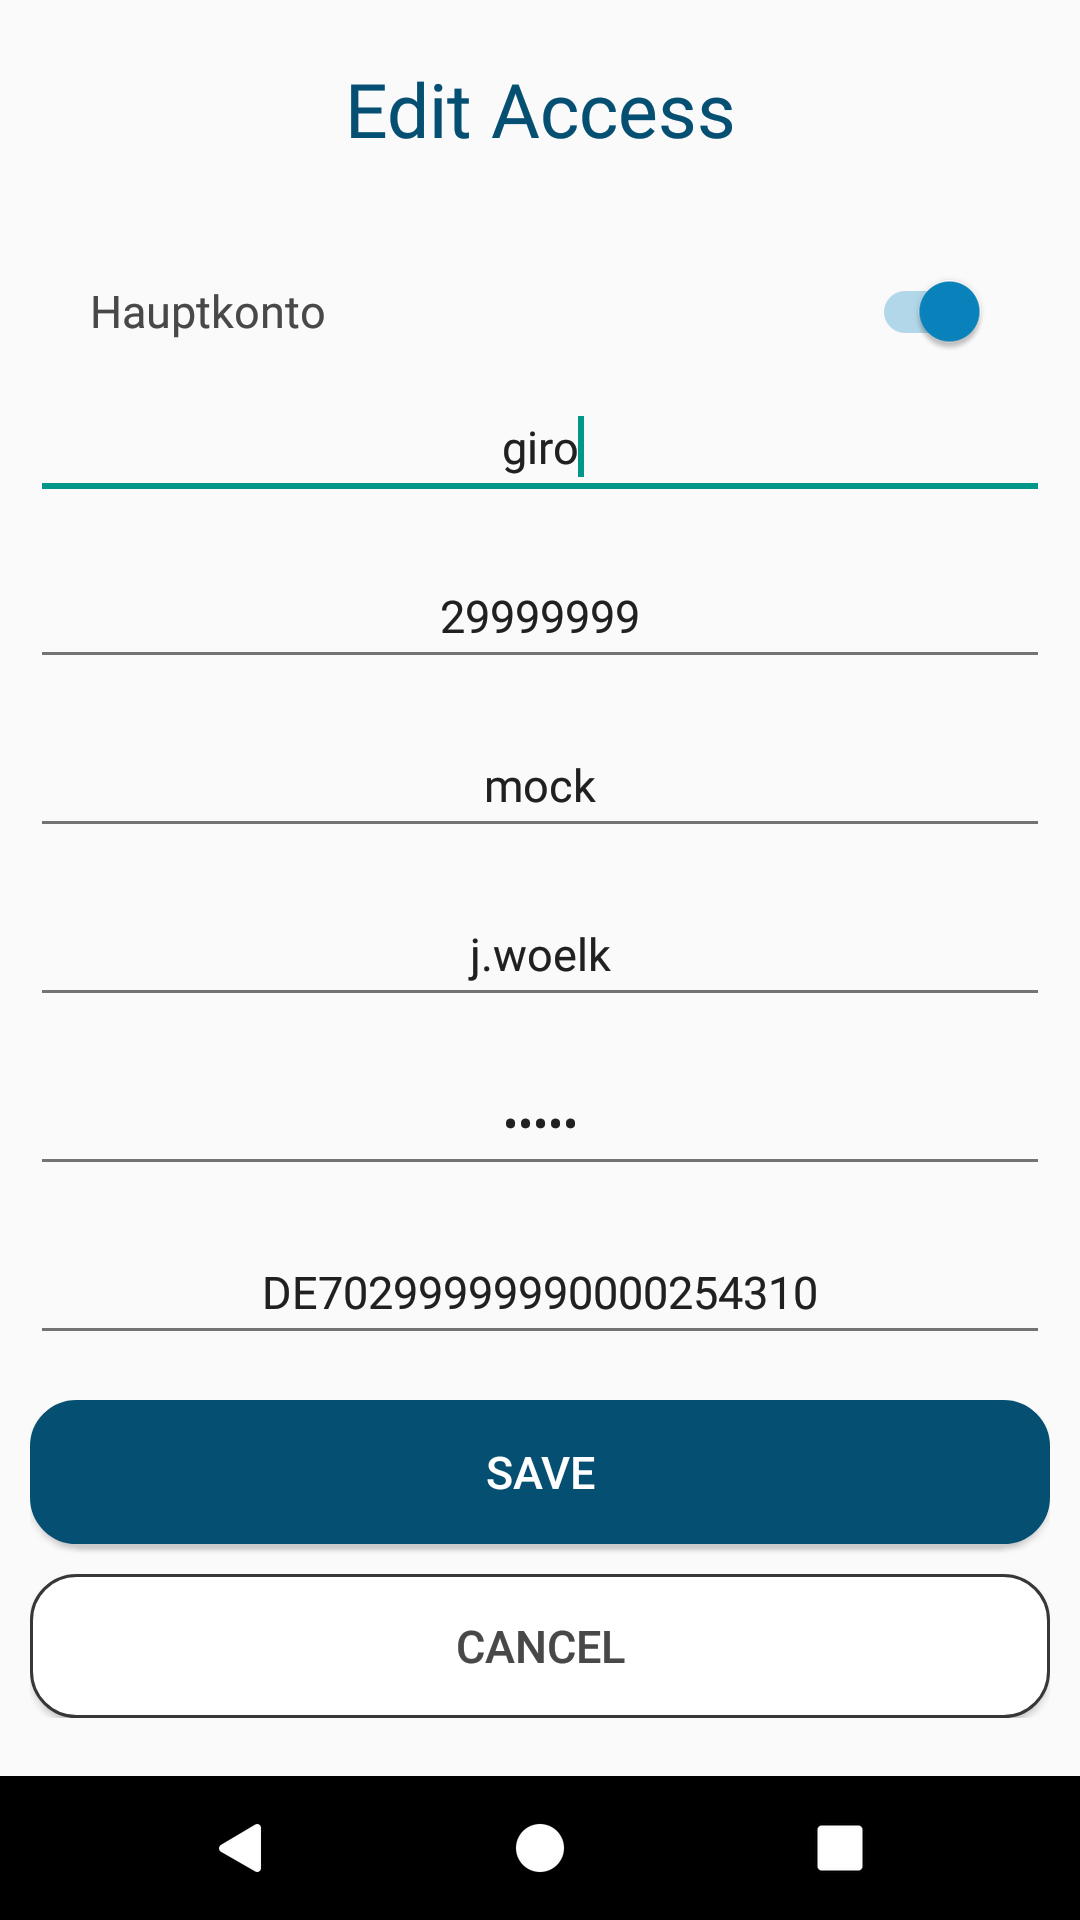
\includegraphics[width=\textwidth]{bilder/4_appMainAccount.png}
  \end{minipage}
  \caption{Bildschirm zur Anzeige und Bearbeitung der Bankkonten-Anbindungen}
  \label{fig:app-accounts}
\end{figure}

Jeder Datensatz wird in einem eigenen Reiter organisiert. Die Oberfläche für die Bearbeitung einer Anbindung wird rechts in Abbildung \ref{fig:app-accounts} dargestellt. Oben rechts ist dort auch die Schaltfläche zu sehen, mit der dieses Konto als „Hauptkonto“ gesetzt werden kann. In der Liste ist ein Hauptkonto durch eine blaue Markierung auf der linken Seite markiert. Falls viele Vorlagen erstellt oder Konten angebunden werden, kann das Suchfeld die Bedienung erleichtern. 

\subsection{Auf Push-Nachrichten reagieren}
\label{subsec:app-push}
Um die Aufforderung der Authentifzierung entgegen zu nehmen und die generierten \acp{TAN} zu empfangen wird Firebase verwendet. Durch Klicken auf die empfangene Push-Nachricht erscheint der Bildschirm mit der Aufforderung zur Bestätigung des Fingerabdruckes. Abbildung \ref{fig:app-auth} zeigt die empfangene Nachricht und den Bildschirm mit der Aufforderung. 

\begin{figure}[h]
  \centering
  \begin{minipage}[b]{0.45\textwidth}
    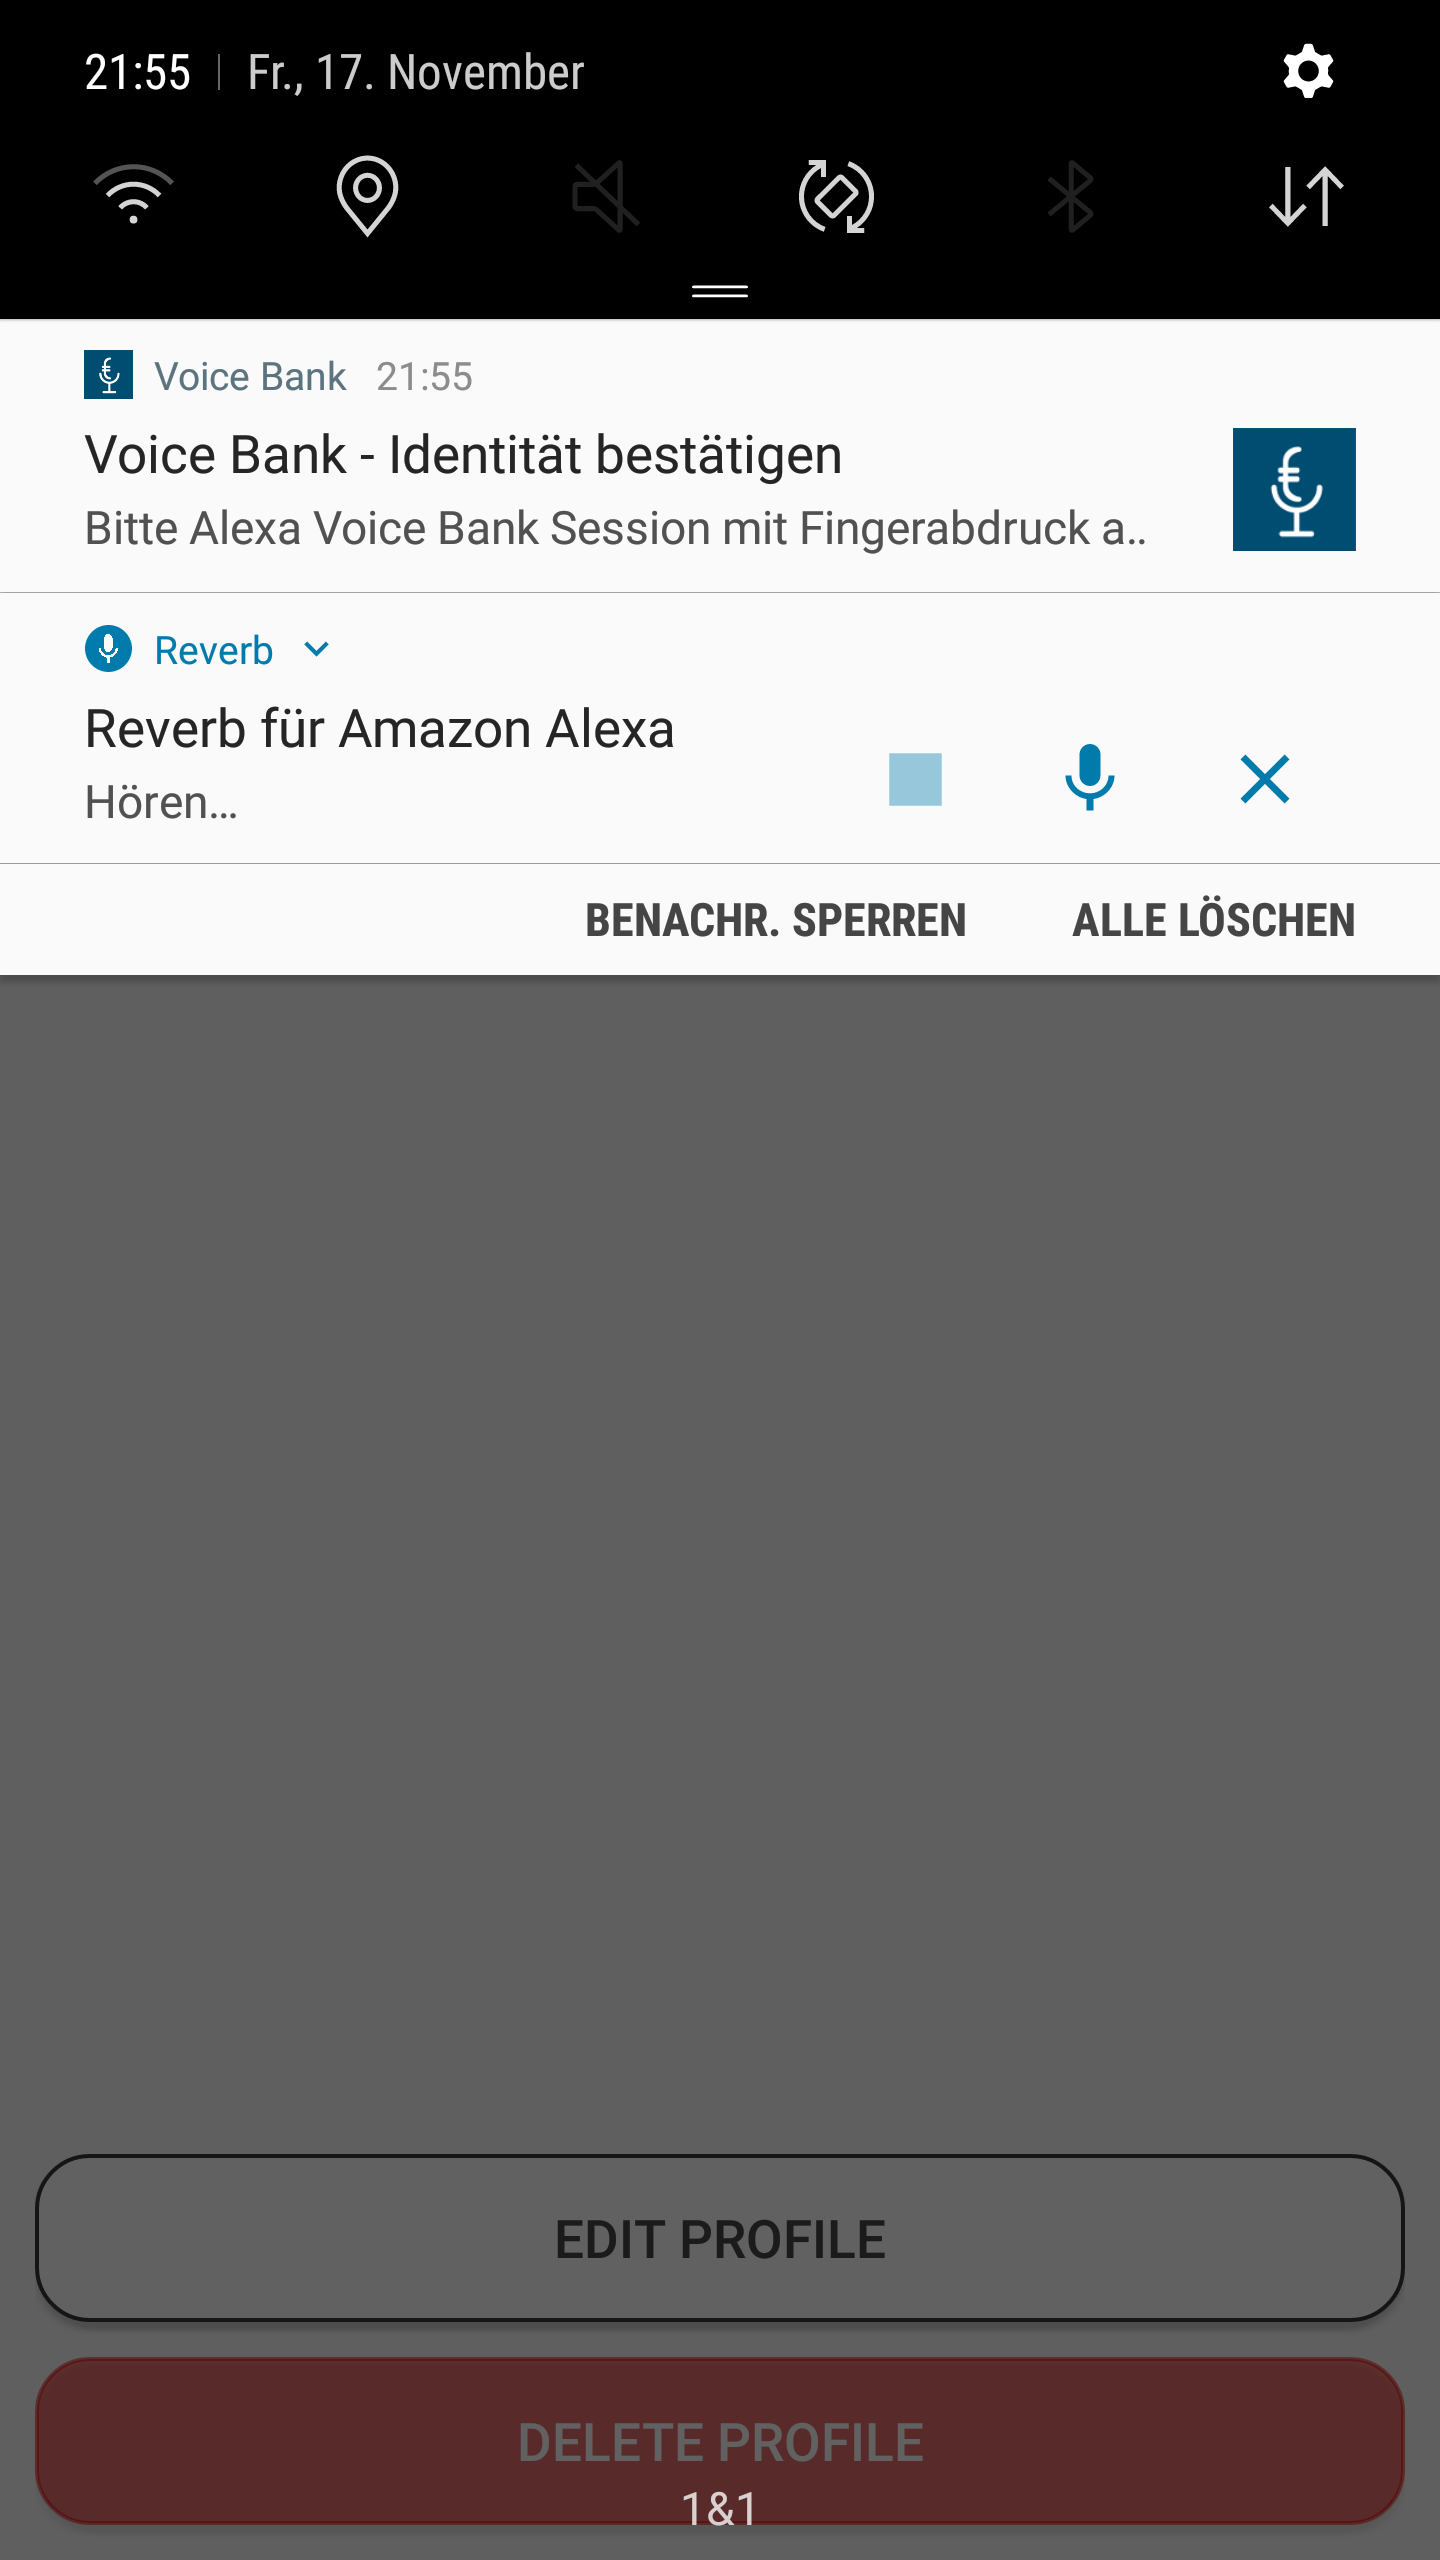
\includegraphics[width=\textwidth]{bilder/4_appPushNachricht.png}
  \end{minipage}
  \begin{minipage}[b]{0.45\textwidth}
    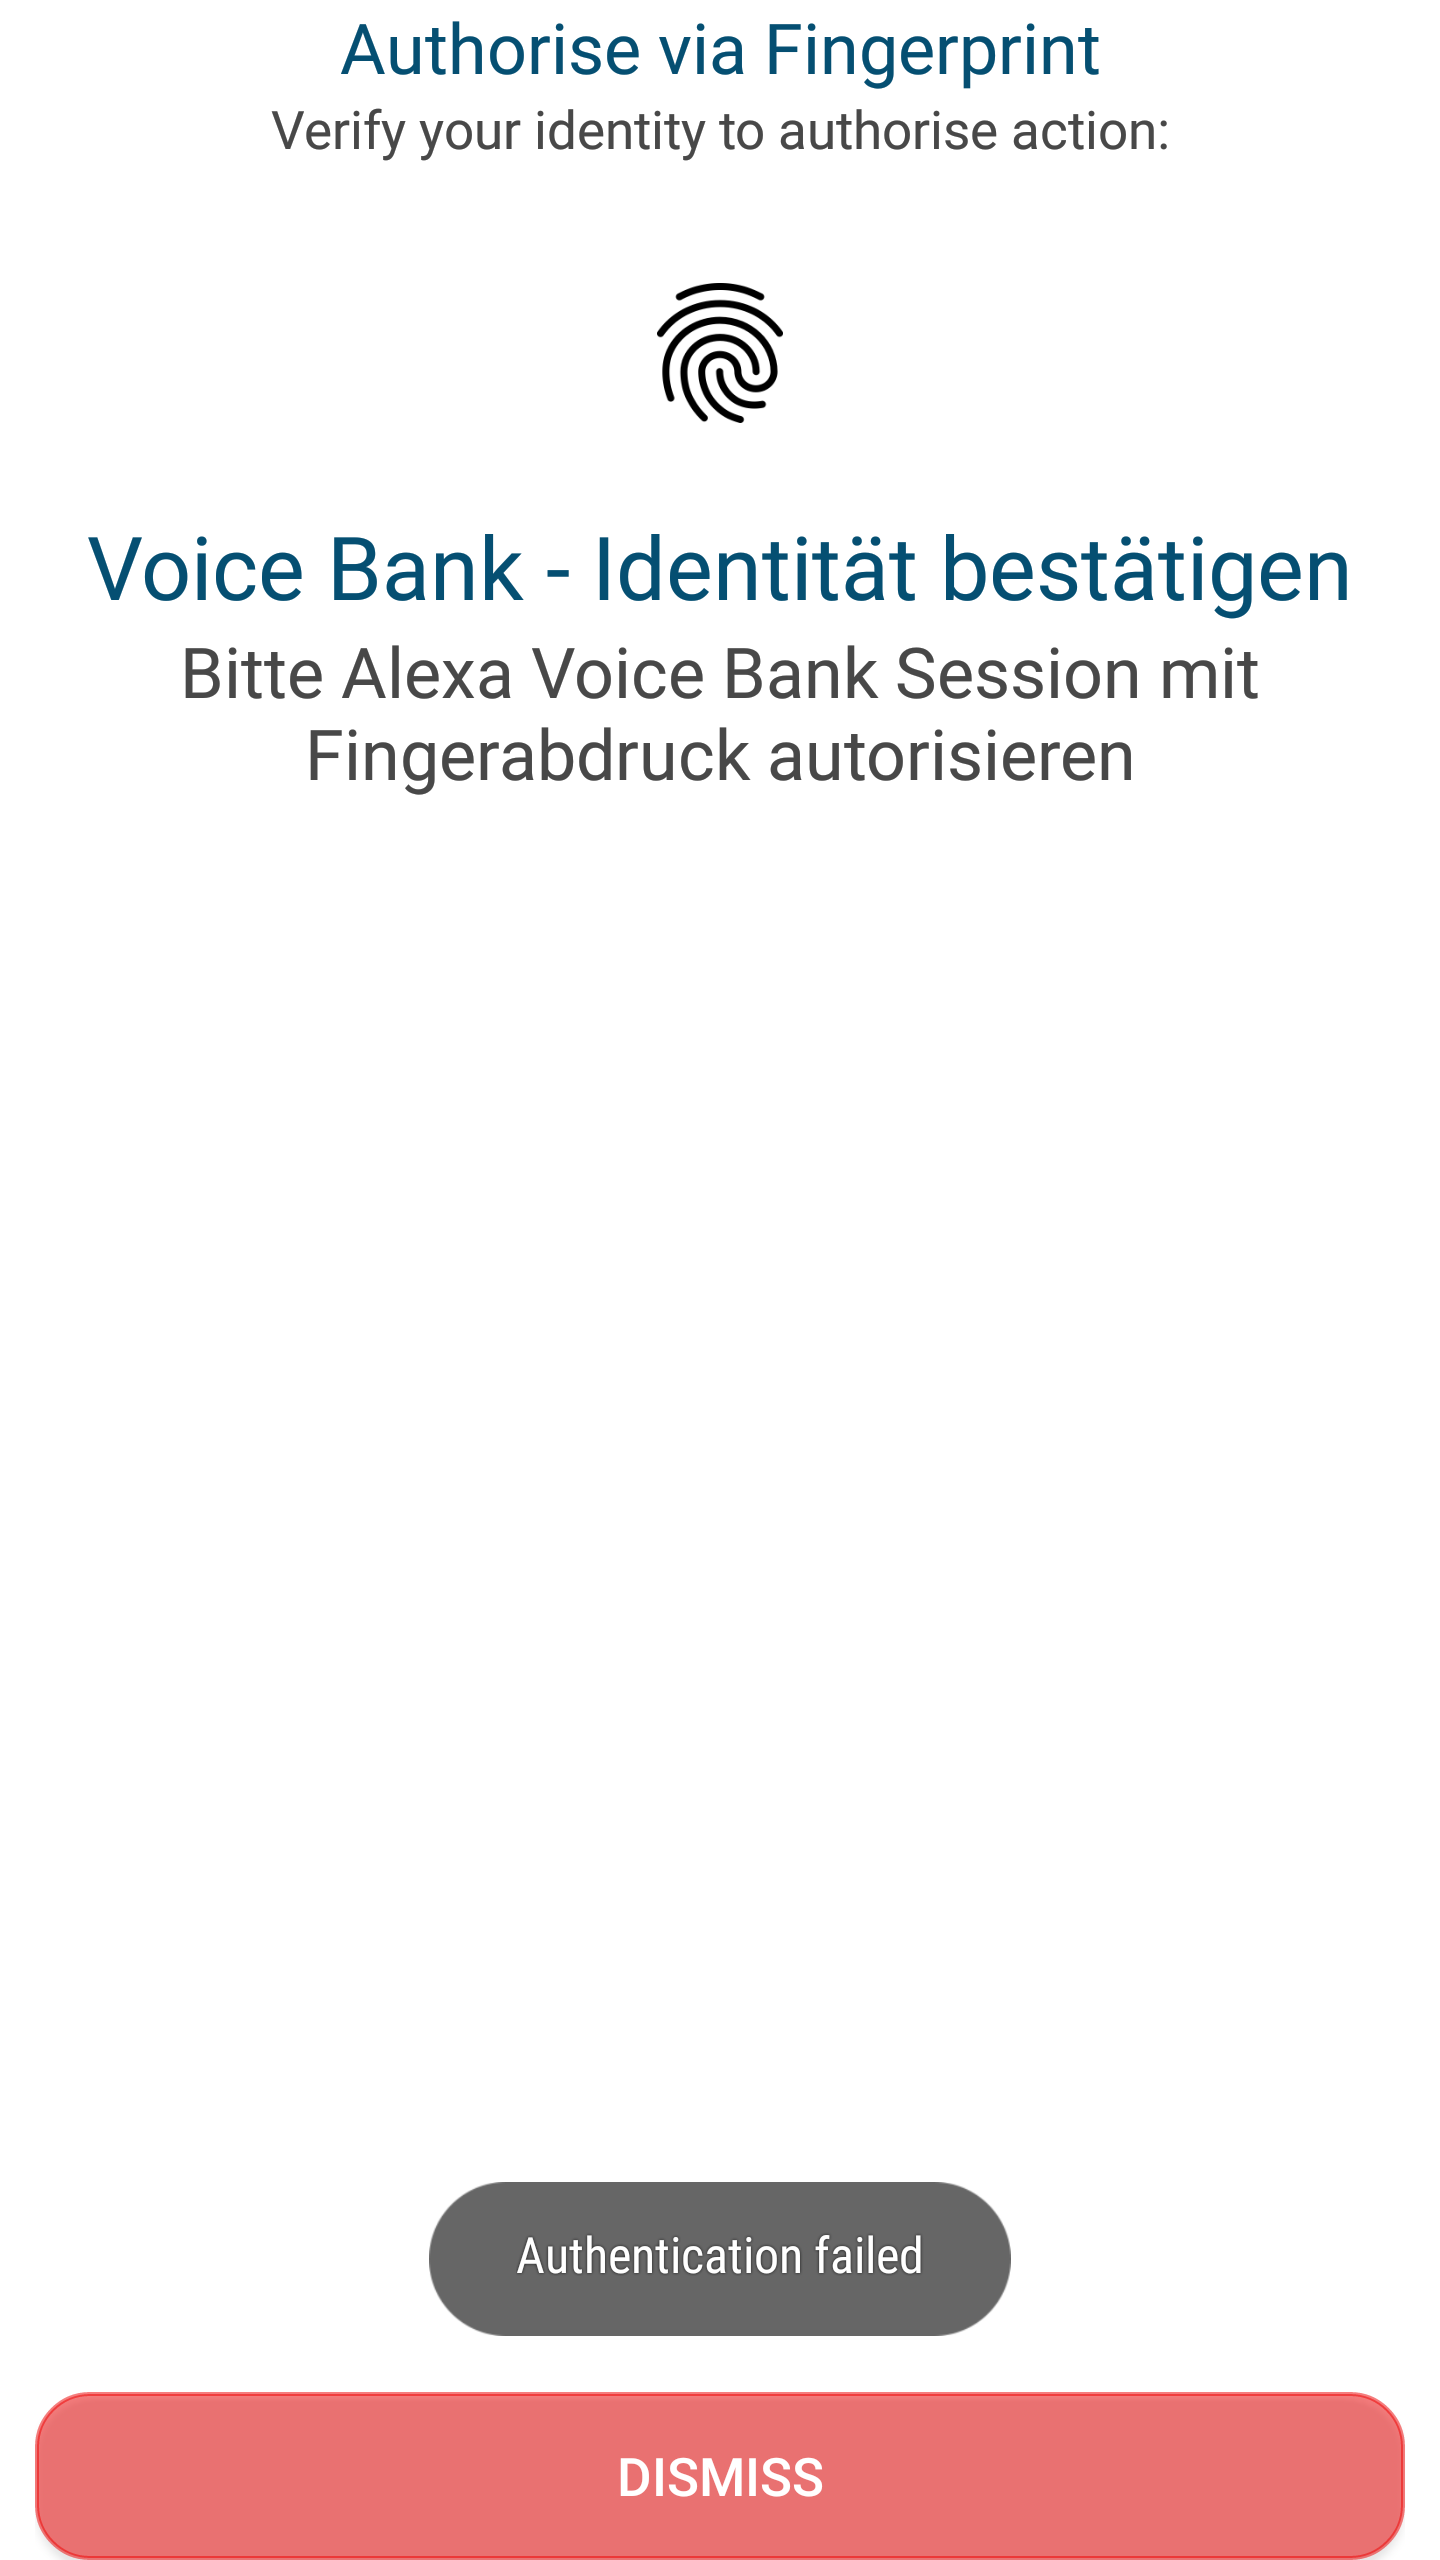
\includegraphics[width=\textwidth]{bilder/4_appAuthorise.png}
  \end{minipage}
  \caption{Bildschirm mit empfangener Push-Benachrichtigung und Aufforderung zur Authentifizierung}
  \label{fig:app-auth}
\end{figure}

Eine empfangene \ac{TAN} Nachricht dient lediglich der Anzeige der Nummer. Durch Klicken wird hier kein neuer Bildschirm geöffnet. Die folgenden Kapitel beschreiben die Implementierung des eigentlichen \ac{CUI}. Der Programmcode der Voice Bank App ist auf der beiliegenden CD unter \textit{„Quelltexte/finlexa\_android/“} zu finden.

\section{Skill-Server}
\label{sec:skill-server}
Aus Kapitel \ref{sec:alexa-voice-service} ist bekannt, dass der Skill-Server die Logik des \ac{CUI} abbildet. Die mit Hilfe des Interaction Model und der \ac{NLP} interpretierten Daten werden an den Skill-Server übermittelt. Hier müssen die entsprechenden Verknüpfungen mit dem Nutzungskontext stattfinden. Des Weiteren ist die Antwort zu generieren, die zurück an die Alexa Plattform geschickt wird. Dafür muss der Skill-Server ebenfalls eine \ac{REST}-Schnittstelle implementieren, die Alexa konsumieren kann. Der Server muss für die Alexa Plattform über das Internet zugänglich sein. Dabei gibt es mehrere Möglichkeiten für die Bereitstellung. Eine ist die Nutzung von \textit{Lambda}, einer sogenannten \textit{\ac{FaaS}}\footnote{FaaS ist ein Dienst, der von Cloud-Plattformen angeboten wird. Er ermöglicht die Entwicklung, Verwaltung und Bereitstellung von Applikationen ohne die sonst benötigte, komplexe Konfiguration einer Server Infrastruktur.}. Lambda ist Teil der \textit{\ac{AWS}} und erleichtert die Bereitstellung eines Skill-Servers in vielerlei Hinsicht. Ein Skill-Server muss verschiedene Voraussetzungen erfüllen, damit er von Alexa genutzt werden kann \cite{alexa-verify-request}.

\begin{itemize}
    \item Er muss über das Internet erreichbar sein
    \item Er muss gemäß der von Amazon definierten \ac{ASK}-Schnittstelle kommunizieren
    \item Er muss \ac{SSL}/\ac{TLS} unterstützen
    \item Er muss Anfragen auf Port 443 akzeptieren
    \item Er muss Anfragen von Alexa validieren
\end{itemize}

Fast alle der Anforderungen werden von Lambda \bzw \ac{AWS} übernommen. Zu erwähnen ist, dass \ac{AWS} nur ein Jahr lang kostenfrei benutzt werden kann\footnote{Mittlerweile kann AWS über das erste Jahr hinaus verwendet werden, wenn der Datenverkehr ein bestimmtes Kontingent nicht überschreitet}. Man ist jedoch nicht auf dessen Nutzung angewiesen. Für die Bereitstellung kann man jede Art von Web-Server verwenden, die diese Anforderungen erfüllt. Der Skill-Server wird in dieser Arbeit ebenfalls über einen eigenen Server bereitgestellt. Der Grund dafür ist in erster Linie, diese Art der Bereitstellung einmal selbst durchgeführt zu haben. Des Weiteren kann die Infrastruktur des Projektträgers ohne zusätzlichen Kostenaufwand verwendet werden. Der Prozess ist in Kapitel \ref{sec:deployment} näher beschrieben. Die Nutzung von Lamba wird hier nicht dokumentiert. Es gibt bereits zahlreiche Tutorials und Anleitungen, die sich im Detail damit beschäftigen \cite{aws-lambda}. Im nächsten Kapitel wird das \ac{ASK}-\textit{\ac{SDK}}\footnote{Ein \ac{SDK} ist typischerweise eine Ansammlung von Tools und bereits geschriebenem Programmcode, die bei der Entwicklung von Software-Anwendungen unterstützen.} vorgestellt. 

\subsection{Alexa Skills Kit SDK}
\label{subsec:skill-ask-sdk}
Ein gängiges Mittel für die Entwicklung eines Alexa Skills ist die Verwendung des \ac{ASK}-\ac{SDK} \cite{alexa-sdk}. Es stellt viele Dinge bereit und erleichtert damit den Entwicklungsprozess. Die folgenden Funktionalitäten sind \ua Teil des \ac{SDK}.

\begin{itemize}
    \item \textit{Request handling}: Es unterstützt bei der Verarbeitung der eingegangenen Anfragen von Alexa. \ac{JSON} Daten werden bereits geparsed, das heißt für die weitere Verarbeitung als nutzbares Objekt angeboten. Für definierte Intents kann man auf einfache Weise die Funktionen mit der entsprechenden Logik adressieren.
    
    \item \textit{Session handling}: Da \ac{REST} im Allgemeinen zustandslos ist, erfolgt die Interaktion mit einem Skill in sogenannten Sessions. Es handelt sich dabei um ein Objekt, welches relevante Daten im Zuge einer Konversation speichern kann. In der Regel ist eine Session vom Start des Skills bis zu dessen Beendigung aktiv. Das \ac{SDK} unterstützt beim Handhaben des Session-Objektes. Konkret vereinfacht es die Erstellung und Bearbeitung. 
    
    \item \textit{State handling}: Ein Skill kann verschiedene Zustände einnehmen. Diese können frei vom Entwickler definiert werden. Auch hierbei unterstützt das \ac{SDK} bei der Handhabung dieser Stati. 
    
    \item \textit{Response building}: Die \ac{ASK} Schnittstelle arbeitet unter Verwendung einer definierten \ac{JSON} Syntax. Sowohl Anfragen von Alexa, als auch die Antworten müssen diesem Schema entsprechen \cite{alexa-response-request-format}. Unter Verwendung des \ac{SDK} müssen lediglich die Antworten selbst generiert werden. Es erstellt im Anschluss die notwendigen Strukturen für die Antwort.
\end{itemize}

Auch wenn es sichtlich viele Vorteile bietet, ist die Nutzung des \ac{SDK} auch mit einer gewissen Einschränkung verbunden. Bei der Entwicklung muss man den vorgegebenen Paradigmen folgen. Gerade beim Verarbeiten der eingegangenen Anfragen hat man als Entwickler erst spät Einfluss auf den weiteren Weg der Anfrage. Der Einstiegspunkt sind die für die Intents adressierten Funktionen, auch Handler genannt. Da das Bewusstsein für den Kontext eine der Anforderungen an das \ac{CUI} ist (\vgl Kapitel \ref{sec:conversational-user-interface}), soll der Skill-Server auch dementsprechend kontextbasiert agieren. Das erfordert die Anfrage auszuwerten und selbst zu entscheiden, welche Handler für diesen Kontext in Frage kommen. Eine weitere Einschränkung gilt der Auswertung der Slots, was gerade für den Banking Skill ein Problem darstellt. Für ein besseres Verständnis wird dies anhand eines Beispiels erklärt.\\
Hierfür werden die Intents „Transaktion via Vorlage“ und „Sparziel“ verwendet. Beide benötigen einen „Name“ Slot für die Verarbeitung. Für die Transaktion ist das der Name der verwendeten Überweisungsvorlage, während das Sparziel den Namen des Themas benötigt, für das gespart werden soll. Aus Kapitel \ref{sec:alexa-voice-service} ist bekannt, dass sämtliche Formulierungen für Alexa vorgegeben werden müssen. Das schließt auch die Formulierungen ein, die Benutzer im Fall von fehlenden Slots verwenden. Auch wenn das Interaction Model in Kapitel \ref{sec:interaction-model} beschrieben ist, wird hier für das Verständnis eine Erklärung benötigt. Eine Utterance für das Beispiel der Transaktion wäre:\\\\
Transaktion \textit{Überweise \{Betrag\} an \{Name\}}
\\\\
An erster Stelle steht der Intent, der über die angegebene Formulierung angesprochen wird. Danach ist die eigentliche Formulierung mit ihren Slots, hier „Betrag“ und Name“, gegeben. Die Möglichkeit besteht, dass ein Nutzer lediglich den Betrag nennt. Der Skill sollte dann auf den fehlenden Namen aufmerksam machen und \zB das Folgende ausgeben:
\begin{center}
   \textcolor{mybluelight}{Alexa: „An wen möchtest du überweisen?“}
\end{center}
Gemäß den User Tests aus Kapitel \ref{sec:prototyping}, hat jeder Benutzer diese Frage alleine mit dem entsprechenden Namen beantwortet. Die Utterance hierfür sieht also folgendermaßen aus:\\\\
Transaktion\textit{\{Name\}}\\\\
Denkt man nun an alle Intents, die einen derartigen Slot beinhalten, wie \zB der Sparziel Intent oder der Intent für Informationen zu Umsatzdaten, sehen deren Utterances für diesen Fall identisch aus.\\\\
    Transaktion \textit{\{Name\}}\\
    Sparziel \textit{\{Name\}}\\
    UmsatzInformation \textit{\{Name\}}\\\\
Alexa kann Intents lediglich anhand der im Interaction Model hinterlegten Formulierungen unterscheiden. An dieser Stelle gibt es also ein Problem. Nennt ein Benutzer einen Namen, kann Alexa nicht differenzieren, welcher der Intents angesprochen werden muss. Größtenteils wird der erste angesprochen, der mit der Eingabe übereinstimmt. In diesem Fall ist das die Transaktion. Aus den genannten Gründen wird das \ac{SDK} nicht in dieser Arbeit verwendet\footnote{Im Verlauf dieser Arbeit wurde das \ac{SDK} von Amazon erweitert. Die beschriebenen Einschränkungen können dadurch gelöst werden. Da nach einer Evaluierung der Ansatz aus Kapitel \ref{subsec:skill-architektur} dennoch als flexibler erachtet wird, wurde dieser weiter verfolgt.}. Kapitel \ref{subsec:skill-architektur} beschreibt die Entwicklung einer Architektur, mit deren Hilfe der Skill-Server implementiert werden kann.

\subsection{Architektur}
\label{subsec:skill-architektur}
Aufgrund der in Kapitel \ref{subsec:skill-ask-sdk} genannten Einschränkungen des \ac{SDK}, wird eine Architektur für den Skill-Server entwickelt. Diese soll in erster Linie die beschriebenen Probleme lösen. Abbildung \ref{fig:skill-architektur-komponenten} zeigt das Ergebnis in Form einer Komponentenübersicht.

\begin{figure}[!htb]
    \centering
    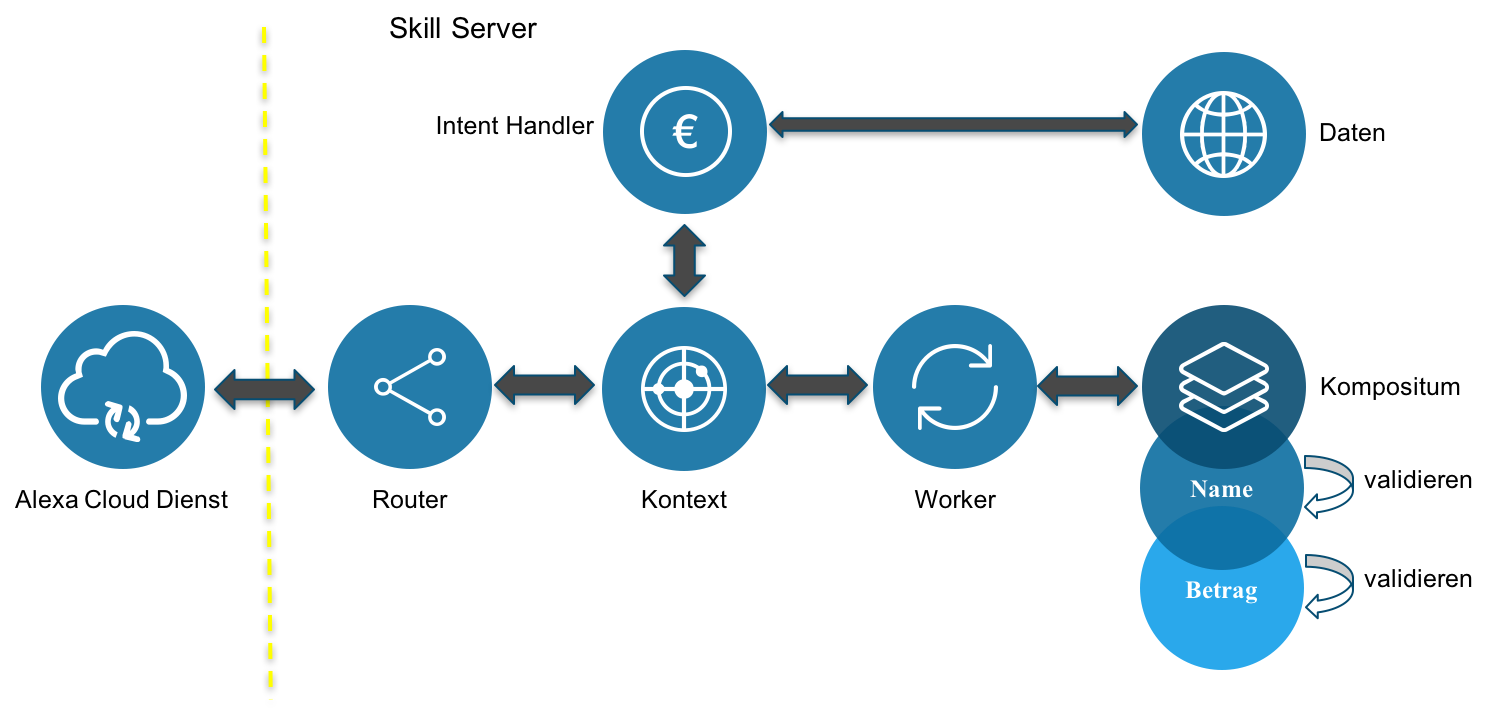
\includegraphics[width=1.0\textwidth]{bilder/4_skillArchitektur.png}
    \caption{Komponentenübersicht der Architektur}
    \label{fig:skill-architektur-komponenten}
\end{figure}

Alexa sendet eine Anfrage an den Skill-Server. Entsprechend der Daten baut dieser den Kontext auf. Der Kontext erstellt auf Basis der für den Intent benötigten Slots und deren Werte eine Worker Instanz. Der Worker hält ein \textit{Kompositum}\footnote{Ein Entwurfsmuster aus der Software Entwicklung \cite{freeman-headfirst-patterns}} mit diesen Slots, die nun sequentiell validiert werden. Falls Slots fehlen oder eingegebene Werte vom Benutzer bestätigt werden müssen, wird die Antwort vom Worker generiert und über den Kontext zurück an die Alexa Plattform gesendet. Bei erfolgreicher Validierung gibt der Worker keine Antwort an den Kontext zurück. Die Parameter werden dann an den Intent Handler übermittelt, worauf dieser ausgeführt wird. Die entsprechende Logik wird durchlaufen und \ggf werden relevante Daten über weitere Dienste beschafft. Im Anschluss generiert er die Antwort und gibt sie dem Kontext zurück. Dieser überträgt die Antwort wiederum an die Alexa Plattform.\\
Der aktuelle Kontext besteht also aus dem Intent und dem Kompositum mit den entsprechenden Slots. Aus Kapitel \ref{subsec:skill-ask-sdk} ist das Alexa Session-Objekt bereits bekannt. Bevor der Skill-Server eine Antwort zurück zur Alexa Plattform sendet, wird dieses mit dem aktuellen Kontext beschrieben. Bei der nächsten Anfrage, kann man auf das gleiche Objekt zurückgreifen. Entsprechend dessen und der neuen Daten vom Benutzer wird ein neuer Kontext aufgebaut, die Slots mit \ggf neuen Werten validiert und der Intent Handler ausgeführt. Geht man zum Problem der Slot Validierung aus Kapitel \ref{subsec:skill-ask-sdk} zurück, bietet dieses Vorgehen eine mögliche Lösung. Anstatt jedem der Intents eine Formulierung mit dem Slot „Name“ zuzuweisen, gibt es einen eigenen Intent für diesen Slot. Im Interaction Model sieht das folgendermaßen aus: \\\\
Transaktion \textit{Überweise \{Betrag\} an \{Name\}}\\
Name \textit{\{Name\}}\\
Betrag \textit{\{Betrag\}}\\

Nennt ein Benutzer lediglich den fehlenden Namen, gibt es nur noch einen Intent, der angesprochen werden kann. Diese speziellen Intents werden im Folgenden als \textit{Atomic Intents} bezeichnet. Der Wert des Slots kann nun vom Skill-Server kontextbezogen verarbeitet und an den richtigen Intent Handler adressiert werden. Im Falle einer Transaktion wird der Atomic Intent „Name“ als Name der verwendeten Überweisungsvorlage gehandhabt. Man kann also sagen, dass das Kompositum in Abbildung \ref{fig:skill-architektur-komponenten} aus Atomic Intents zusammengesetzt wird. Kapitel \ref{subsec:skill-implementierung} beschreibt die Umsetzung der hier beschriebenen Architektur. 

\subsection{Implementierung}
\label{subsec:skill-implementierung}
Im Folgenden wird der Skill-Server auf Basis der in Kapitel \ref{subsec:skill-architektur} beschriebenen Architektur umgesetzt. Wie das Backend, ist der Skill-Server mit Node.js, Express und TypeScript implementiert. Die Gründe dafür sind in Kapitel \ref{backend-plattform} genannt. Node.js ist für die Skill Entwicklung die am weitesten verbreitete  Plattform. Erwähnenswert sind außerdem zwei weitere \ac{npm} Module, die hier verwendet werden. 

\textbf{Bespoken Tools}\\
Dabei handelt es sich um einen Verbund an Tools, welche die Entwicklung von Alexa und Google \ac{VUI} Anwendungen unterstützen \cite{bespoken}. Unabhängig davon, ob man den Skill über \ac{AWS} oder einem eigenen Web Server bereitstellt, nimmt der Prozess der Auslieferung (Deployment) einige Minuten in Anspruch. Um Zeit zu sparen ist es wesentlich angenehmer lokal zu entwickeln und zu testen. Da ein Skill-Server über das Internet für Alexa erreichbar sein muss, ist das normalerweise nicht möglich. Mit Hilfe der Bespoken Tools kann genau das erreicht werden, indem ein Proxy Dienst eingerichtet wird. Die Konfiguration dauert nur wenige Minuten und wird mit Hilfe der Kommandozeile durchgeführt. Das Tool gibt eine \textit{\ac{URL}} aus. Diese wird auf der Alexa Plattform als Adresse des Skill-Servers eingetragen. Startet man nun den Proxy und Skill-Server lokal, kann Alexa diese über den Proxy Dienst erreichen und nutzen, zu sehen in  Abbildung \ref{fig:bst-proxy} \cite{bespoken}.

\begin{figure}[!htb]
    \centering
    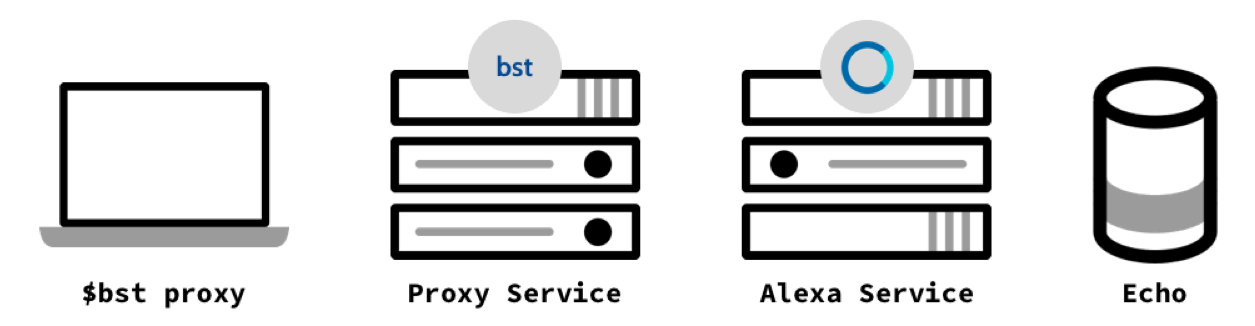
\includegraphics[width=0.8\textwidth]{bilder/4_bstProxy.png}
    \caption{Bespoken Tools Proxy Dienst}
    \label{fig:bst-proxy}
\end{figure}

Der Proxy ist nur eine der Anwendungen von Bespoken. Auf Weitere wird im Zuge dieser Arbeit nicht eingegangen, da lediglich die hier beschriebene verwendet wird.

\textbf{Alexa Verifier Middleware}\\
Mit Hilfe dieses Moduls können Anfragen von Alexa validiert werden \cite{alexa-verify-request}. Somit werden einige der in Kapitel \ref{sec:skill-server} genannten Voraussetzung eines Skill-Servers erfüllt. Mit Hilfe von Express kann dieses Modul über zwei Zeilen Quelltext eingesetzt werden. 

\textbf{Umsetzung}\\
Im Anschluss folgt die Umsetzung der in Kapitel \ref{subsec:skill-architektur} beschriebenen Architektur. Angefangen mit einer groben Übersicht in Abbildung \ref{fig:skill-komponenten}, werden die hellblau hinterlegten Komponenten im weiteren Verlauf näher beschrieben. Die Übersicht aus Kapitel \ref{subsec:skill-architektur} unterscheidet sich von der hier gezeigten Abbildung und stellt lediglich den Anfangsgedanken der Implementierung dar. Die Unterschiede in Abbildung \ref{fig:skill-komponenten} sind auf die Gegebenheiten der verwendeten Plattform und auf die Weiterentwicklung dieses Gedankens zurückzuführen.

\begin{figure}[!htb]
    \centering
    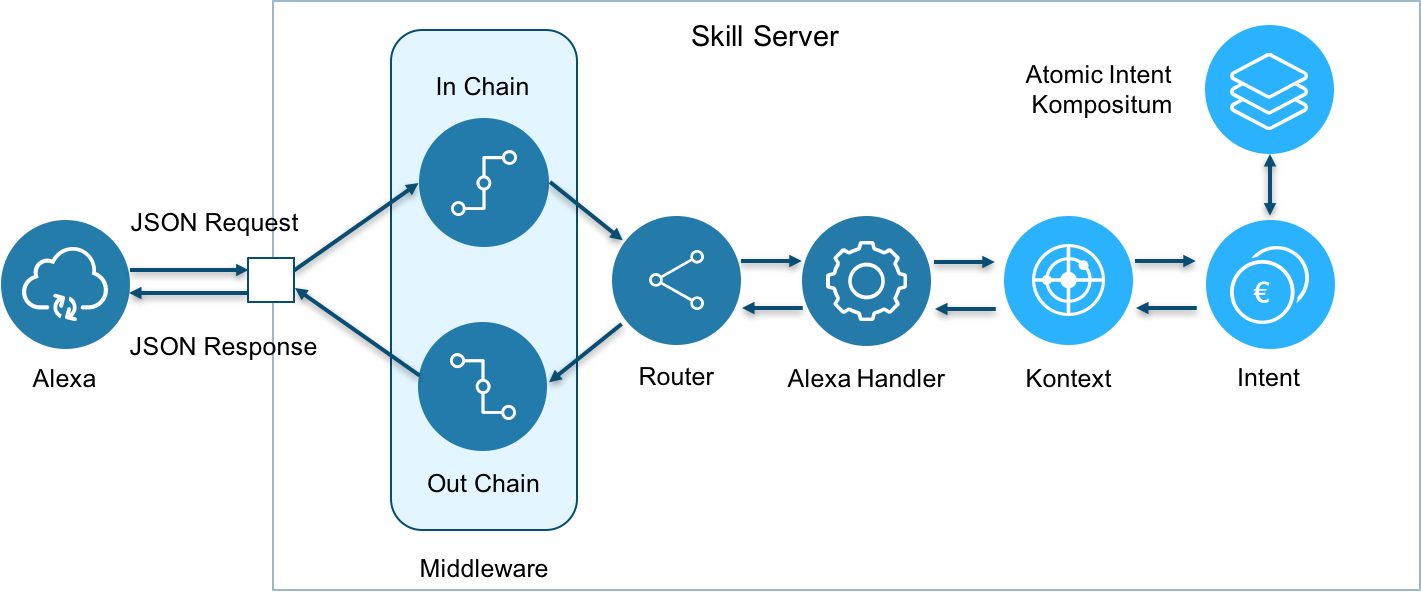
\includegraphics[width=1.0\textwidth]{bilder/4_skillKomponenten.png}
    \caption{Komponentenübersicht des Skill-Servers}
    \label{fig:skill-komponenten}
\end{figure}

Alexa sendet eine \ac{JSON} Anfrage (Request) an den Endpunkt des Servers. Die Anfrage passiert zunächst die Middleware. Diese besteht zum einen aus der „In Chain“, die \ua die beschriebene Alexa Verifier Middleware enthält. Zum anderen aus der „Out Chain“, welche die Antwort (Response) des Skills lediglich weitergibt. Der Router leitet die Request entsprechend ihres Ziels zur registrierten Handler Funktion. Hier gibt es nur eine Route, die den Alexa Handler adressiert. Dieser erstellt mit Hilfe der Daten aus der Request den Kontext. Die Daten umfassen \ua das Session-Objekt und die analysierten Informationen der Alexa \ac{NLP} mit dem vom Benutzer angesprochenen Intent, enthaltenen Slots und deren Werte. Ist der Kontext erstellt, wird dieser vom Alexa Handler ausgeführt.\\
Über den Kontext wird ein Intent erzeugt. Dieser baut wiederum sein Kompositum aus Atomic Intents auf, welches mit den übergebenen Slot Werten validiert wird. Außerdem hält der Intent die Logik. Nach der Validierung des Kompositums entscheidet diese, ob Daten vom Multibanking-Mock beschafft werden müssen und welche Antwort generiert wird. Die Antwort wird über den Kontext an den Handler zurückgegeben. Der Alexa Handler bettet die Phrasen in die \ac{JSON} Syntax ein, die Alexa verstehen kann. Dabei wird auch das Session-Objekt mit dem aktuellen Kontext beschrieben. Das \ac{JSON} Response Objekt wird dann über die Out Chain der Middleware zurück an Alexa gesendet und vom Echo ausgegeben. Im Folgenden werden mit Hilfe von Klassen- und Sequenzdiagrammen die Abhängigkeiten und Prozesse der in Abbildung \ref{fig:skill-komponenten} hellblau hinterlegten Komponenten näher betrachtet. Für einen besseren Überblick wird die Architektur dabei in kleinere Ausschnitte zerlegt.\\
Die Namen der Klassen, Funktionen und Typen in den Diagrammen sind den englischen Begriffen aus der Implementierung nachempfunden. Abbildung \ref{fig:skill-klassen-kontext} zeigt ein Klassendiagramm, dass die Kontext und Intent Komponenten aus Abbildung \ref{fig:skill-komponenten} näher beschreibt. 

\begin{figure}[!htb]
    \centering
    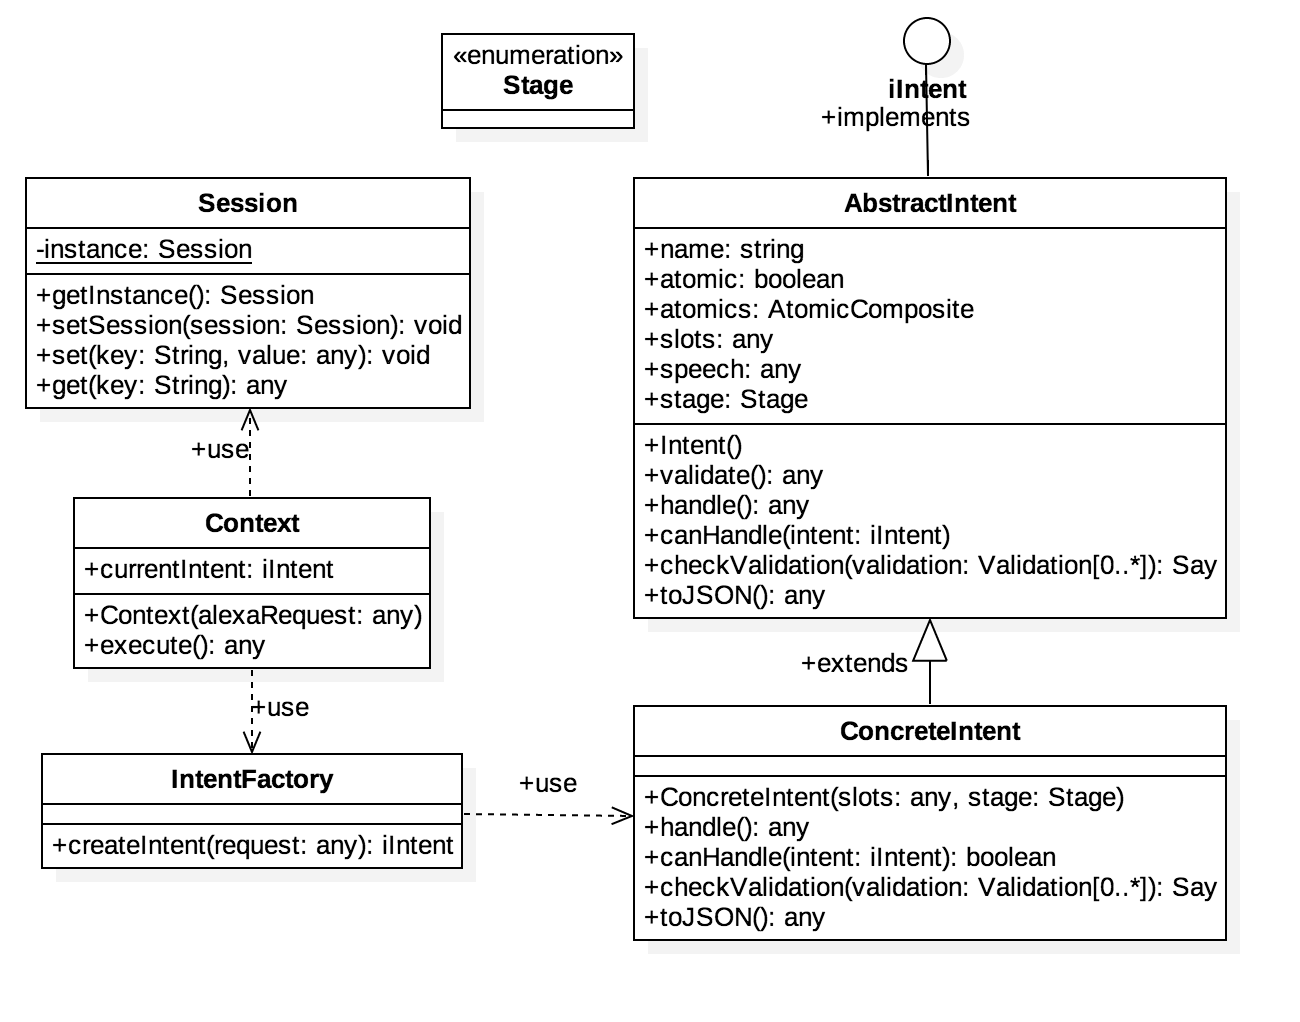
\includegraphics[width=1.0\textwidth]{bilder/4_klassenContext.png}
    \caption{Vereinfachtes Klassendiagramm von Kontext und Intent}
    \label{fig:skill-klassen-kontext}
\end{figure}

Die Kontext Klasse hat einen Konstruktur und die „execute“ Funktion. Im Konstruktor wird zunächst das Session-Objekt der Alexa Request ausgewertet. Die Session Klasse hilft hier beim Auslesen und Modifizieren dieses Objektes. Ist dort noch kein Intent aus vorherigen Interaktionen vorhanden, wird über die Factory ein neuer erstellt und als „currentIntent“ gesetzt. Die Factory ist, wie das Kompositum, ein Entwurfsmuster aus der Softwareentwicklung \cite{freeman-headfirst-patterns}. Sie ist für die Instanziierung eines konkreten Intents zuständig. Nachdem der Kontext erstellt ist, führt der Alexa Handler die execute Funktion aus, die wiederum die „handle“ Funktion des konkreten Intents ausführt. Der Intent gibt entsprechend seiner Logik eine Antwort über den Kontext zurück an den Alexa Handler. Das Sequenzdiagramm aus Abbildung veranschaulicht diesen Prozess.

\begin{figure}[!htb]
    \centering
    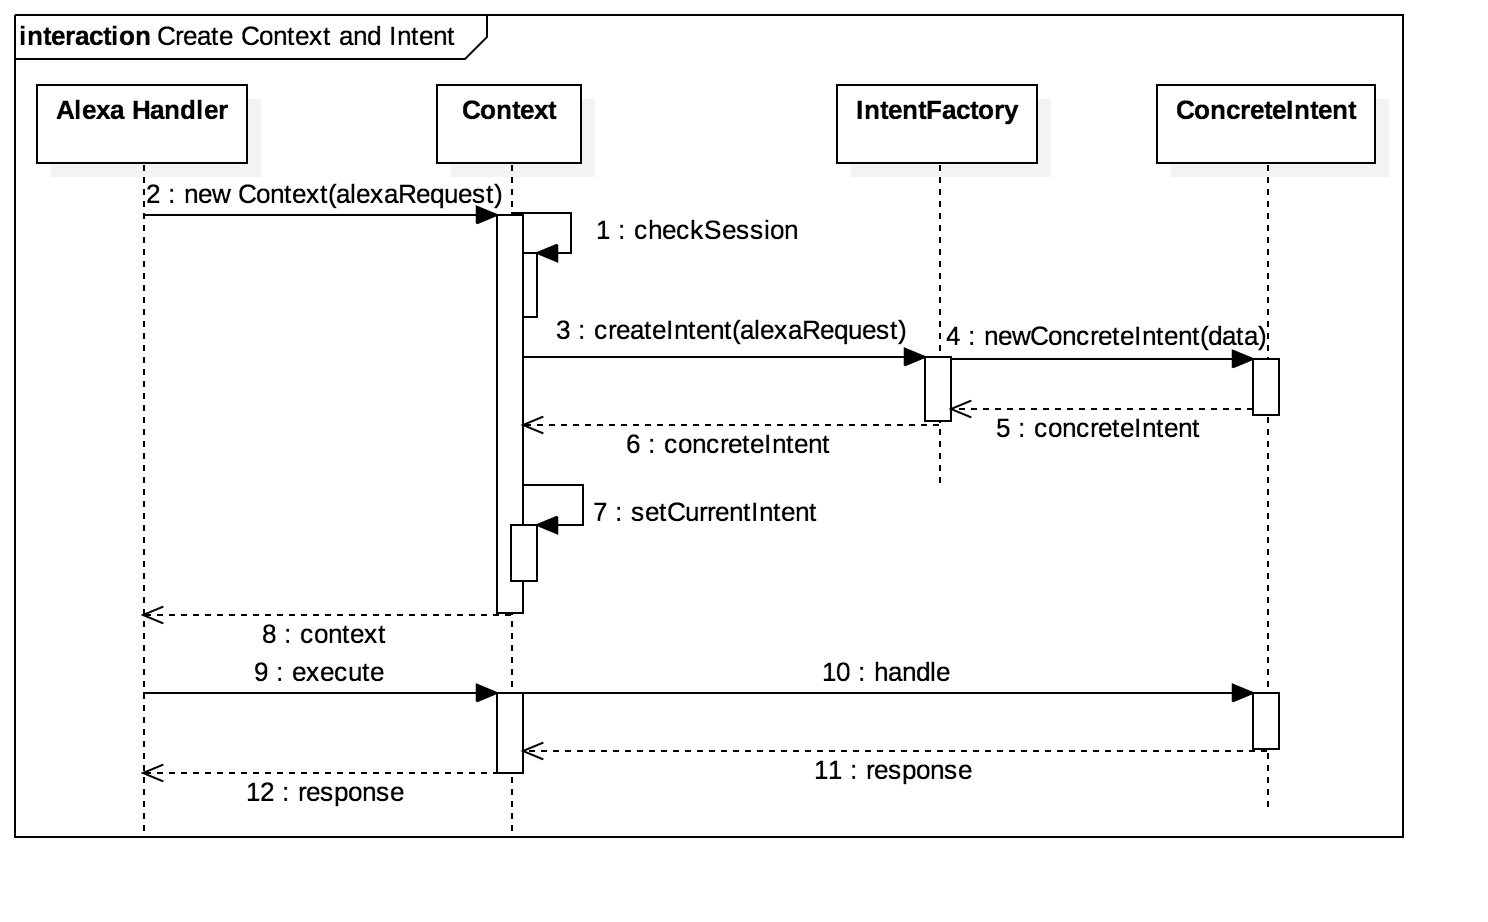
\includegraphics[width=1.0\textwidth]{bilder/4_skillSequenzKontextIntent.png}
    \caption{Sequenzdiagramm Instanziierung von Kontext und Intent}
    \label{fig:skill-sequenz-kontext}
\end{figure}

Im Folgenden wird das Zusammenspiel der Intent und Kompositum Komponente aus Abbildung \ref{fig:skill-komponenten} erläutert. Abbildung \ref{fig:skill-klassen-intent} stellt das entsprechende Klassendiagramm dar.\newpage

\begin{figure}[!htb]
    \centering
    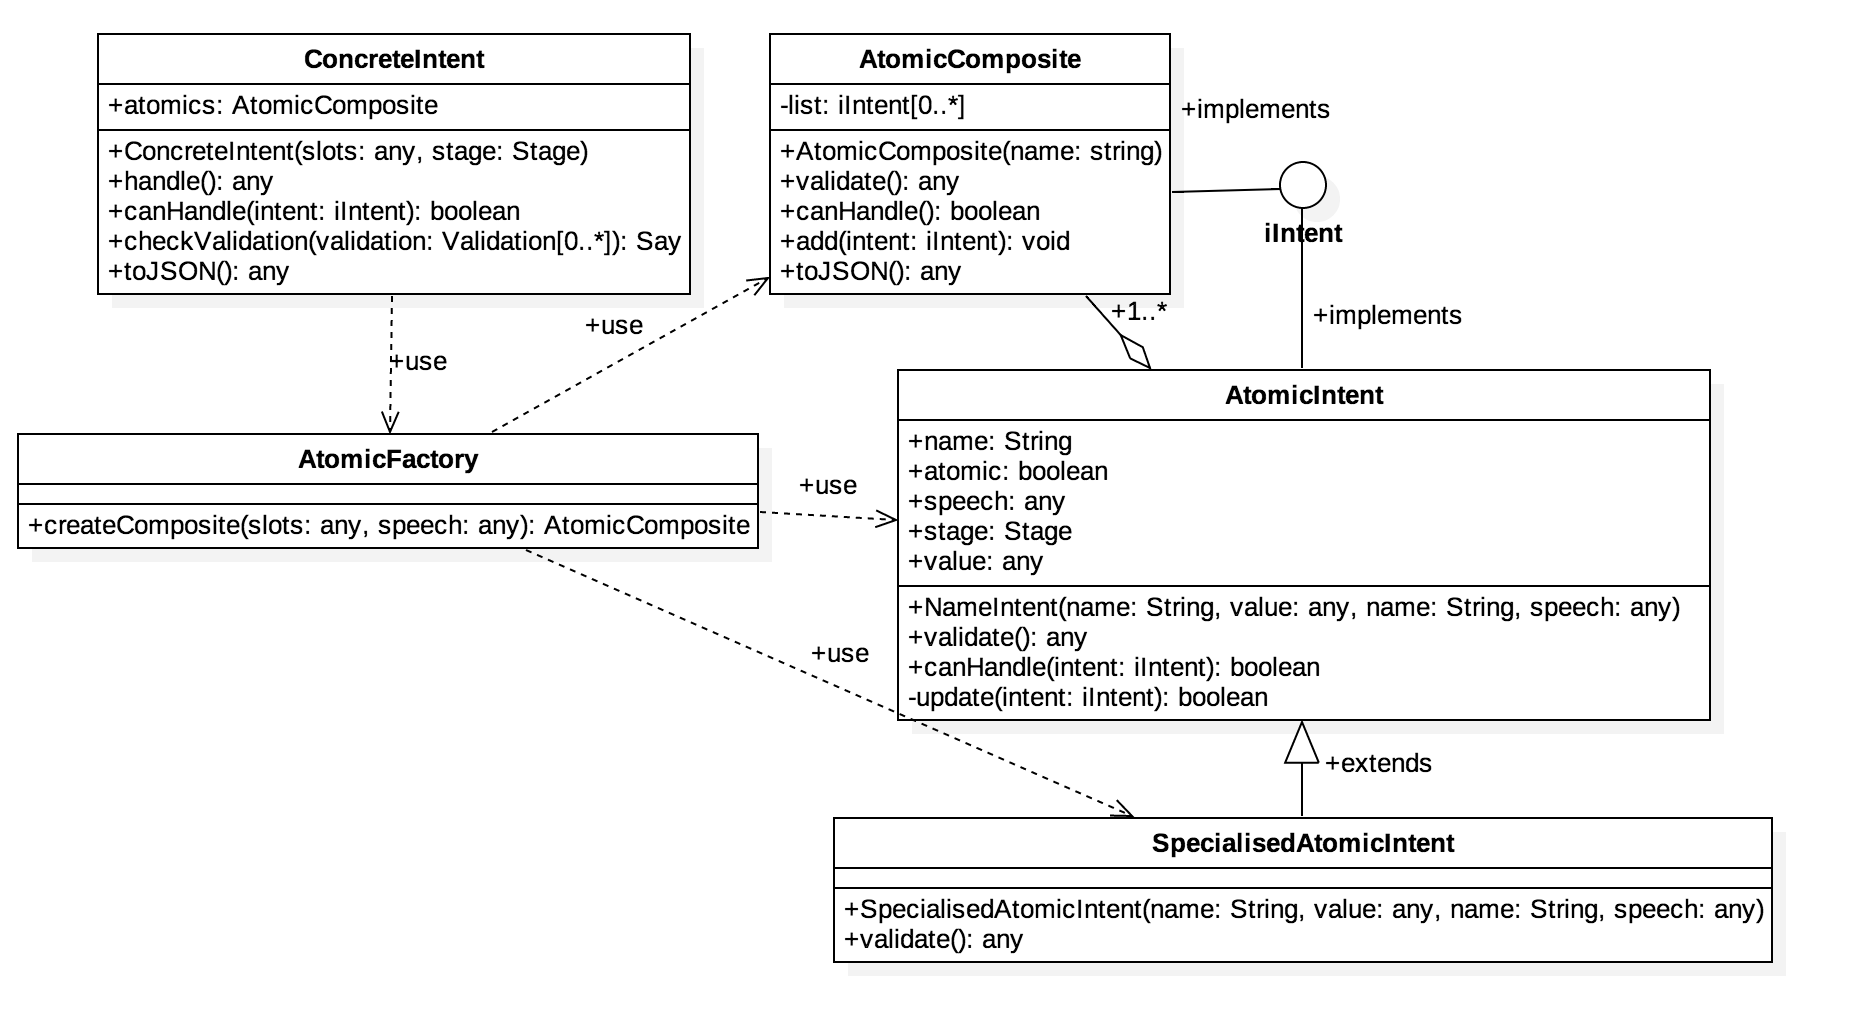
\includegraphics[width=1.0\textwidth]{bilder/4_klassenIntent.png}
    \caption{Vereinfachtes Klassendiagramm von Intent und Atomic Kompositum}
    \label{fig:skill-klassen-intent}
\end{figure}

Konkrete Intents, Atomic Intents und das Atomic Kompositum implementieren das iIntent Interface, dessen wichtigste Eigenschaften und Methoden vorerst erläutert werden.
\begin{itemize}
    \item \textit{atomic}: Legt fest \bzw zeigt an, ob es sich um einen Atomic Intent handelt oder nicht.
    
    \item \textit{speech}: Ein Objekt, dass die Antwortphrasen dieses Intents enthält. Konkrete Intents haben jeweils ein eigenes speech Objekt. 
    
    \item \textit{stage}: Die stage ist eine Enumeration, die verschiedene Stati beschreibt. Bei Atomic Intents dient der Status als Information, ob der Wert validiert wurde, fehlt oder vom Benutzer bestätigt werden muss. Andere Intents wie die Transaktion, die der Nutzer vor deren Durchführung ebenfalls bestätigen muss, greifen auch auf diese Eigenschaft zurück.
    
    \item \textit{value}: Der value ist optional, da er nur von Atomic Intents benötigt wird. Der value enthält den eigentlichen Wert, der über die Slots der Alexa Anfrage gesetzt wird. 
    
    \item \textit{validate()}: Diese Funktion bildet die Logik ab, mit der ein Atomic Intent validiert wird. Je nachdem was validiert werden muss, kann diese Logik variieren.
    
    \item \textit{handle()}: Diese Funktion enthält die Logik eines Intents.
    
    \item \textit{canHandle()}: Die canHandle Funktion wird beim Erstellen des Kontextes verwendet. Ist im Session-Objekt bereits ein Intent enthalten, wird geprüft, ob der Intent aus der Anfrage von diesem gehandhabt werden kann. Ein Beispiel soll dies verdeutlichen. Ein Benutzer hat eine Transaktion angestoßen, jedoch vergessen den Betrag zu nennen. Die Transaktion wird mit dem aktuellen Stand in das Session-Objekt gespeichert. Der Benutzer erhält die Antwort, dass der Betrag fehlt. Spricht der Benutzer nun eine Nummer in den Echo wird dabei der Atomic Intent „Number“ adressiert. Im Kontext wird nun geprüft ob der Transaktions Intent den Number Intent handhaben kann. Da dies der Fall ist, wird der Betrag des Transaktions Intent mit dem Wert des Number Intents aktualisiert.
\end{itemize}

Beim Erstellen eines konkreten Intents wird die Alexa Request an die Intent Factory übergeben. Falls Slots für diesen Intent vorgesehen sind, übergibt die Factory die Daten entsprechend. Innerhalb des konkreten Intent Konstruktors wird eine weitere Factory verwendet, um das Atomic Kompositum aufzubauen. Die Atomic Factory instanziiert ein solches Kompositum und fügt für jeden übergebenen Slot den entsprechenden Atomic Intent hinzu. Aufgrund der Implementierung des iIntent Interfaces, kann das Kompositum von außen als ein Intent Objekt und nicht als Liste behandelt werden. Es spielt dabei keine Rolle ob es nur einen oder viele Atomic Intents enthält. Abbildung \ref{fig:skill-sequenz-kompositum} zeigt das entsprechende Sequenzdiagramm. Es verdeutlicht die Schritte zwischen Sequenz 4 und 5 des Diagrammes aus Abbildung \ref{fig:skill-sequenz-kontext}.\newpage

\begin{figure}[!htb]
    \centering
    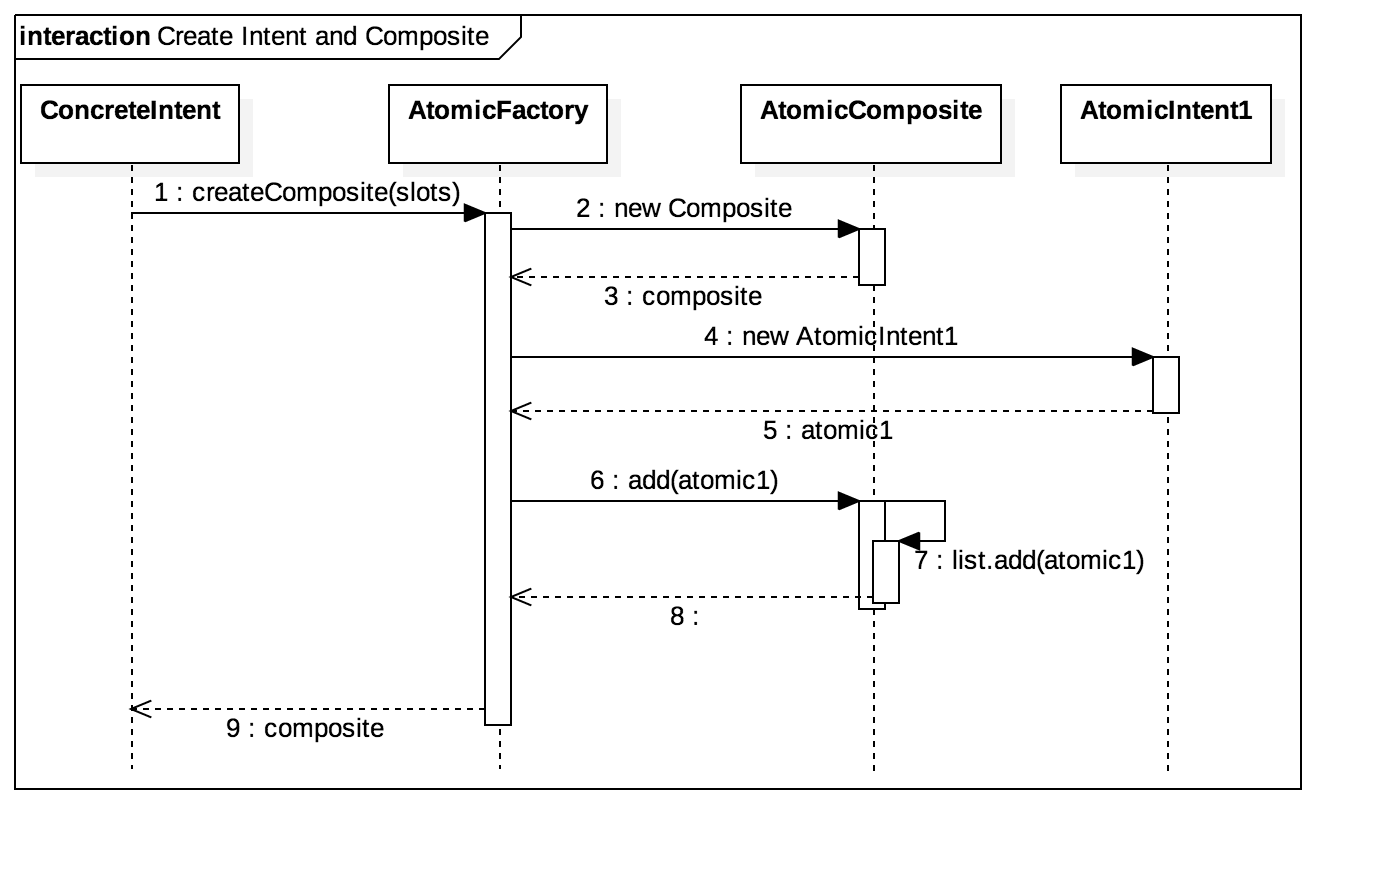
\includegraphics[width=1.0\textwidth]{bilder/4_skillSequenzIntentKompositum.png}
    \caption{Sequenzdiagramm Instanziierung eines Atomic Kompositums}
    \label{fig:skill-sequenz-kompositum}
\end{figure}

Nun sollen die Prozesse zwischen den Schritten 10 und 11 aus dem Sequenzdiagramm in Abbildung \ref{fig:skill-sequenz-kontext} beschrieben werden. Dabei handelt es sich um die Logik \bzw handle Funktion eines konrekten Intents. An dieser Stelle muss man zwischen Intents mit und ohne Slots \bzw Kompositum unterscheiden. Der „Hilfe“ Intent, der keine Slots enthält, gibt lediglich eine der vordefinierten Antworten aus. Sind Slots vorhanden, unterscheiden sich die Methoden je nach Anwendungsfall, dennoch ist ihr grundlegender Aufbau identisch. Zunächst wird die „validate“ Funktion des Kompositums ausgeführt. Sequentiell werden die Ergebnisse jedes Atomic Intents in Form von „Validation“ Objekten einer Liste hinzugefügt, welche zurück an den Intent geht. Diese Objekte umfassen jeweils die Antwortphrase und Stage eines Atomic Intents. Zurück im Intent setzt die „checkValidation“ Methode aus dieser Liste eine Antwort zusammen. Ist die Antwort leer, sind alle Atomic Intents erfolgreich validiert und die handle Logik kann weiter ausgeführt werden. Das Programm holt beispielsweise Daten vom Backend, generiert eine Antwort und gibt diese zurück. Für den Fall, dass die Antwort aus der checkValidation Methode nicht leer ist, beinhaltet sie weitere Rückfragen an den Benutzer. Dabei wird sie direkt und ohne Ausführung der weiteren Logik, an diesen zurückgegeben. Bei den Rückfragen kann es sich um fehlende Slots handeln, die noch eingegeben werden müssen. Falls nötig, wird vor dem Zurückgeben der Antwort der Session Kontext auf den aktuellen Stand gesetzt. Das ist vor allem bei fehlenden Slots der Fall. Diese werden zusammen mit ihren Werten und Stages im Session-Objekt unter dem entsprechenden Intent Namen gespeichert. Stößt der Benutzer den nächsten Schritt der Konversation an, kann der gespeicherte Intent ausgewertet und im neuen Kontext verwendet werden.  Abbildung \ref{fig:skill-sequenz-handle} zeigt die Prozesse der Intent Logik in einem Sequenzdiagramm .

\begin{figure}[!htb]
    \centering
    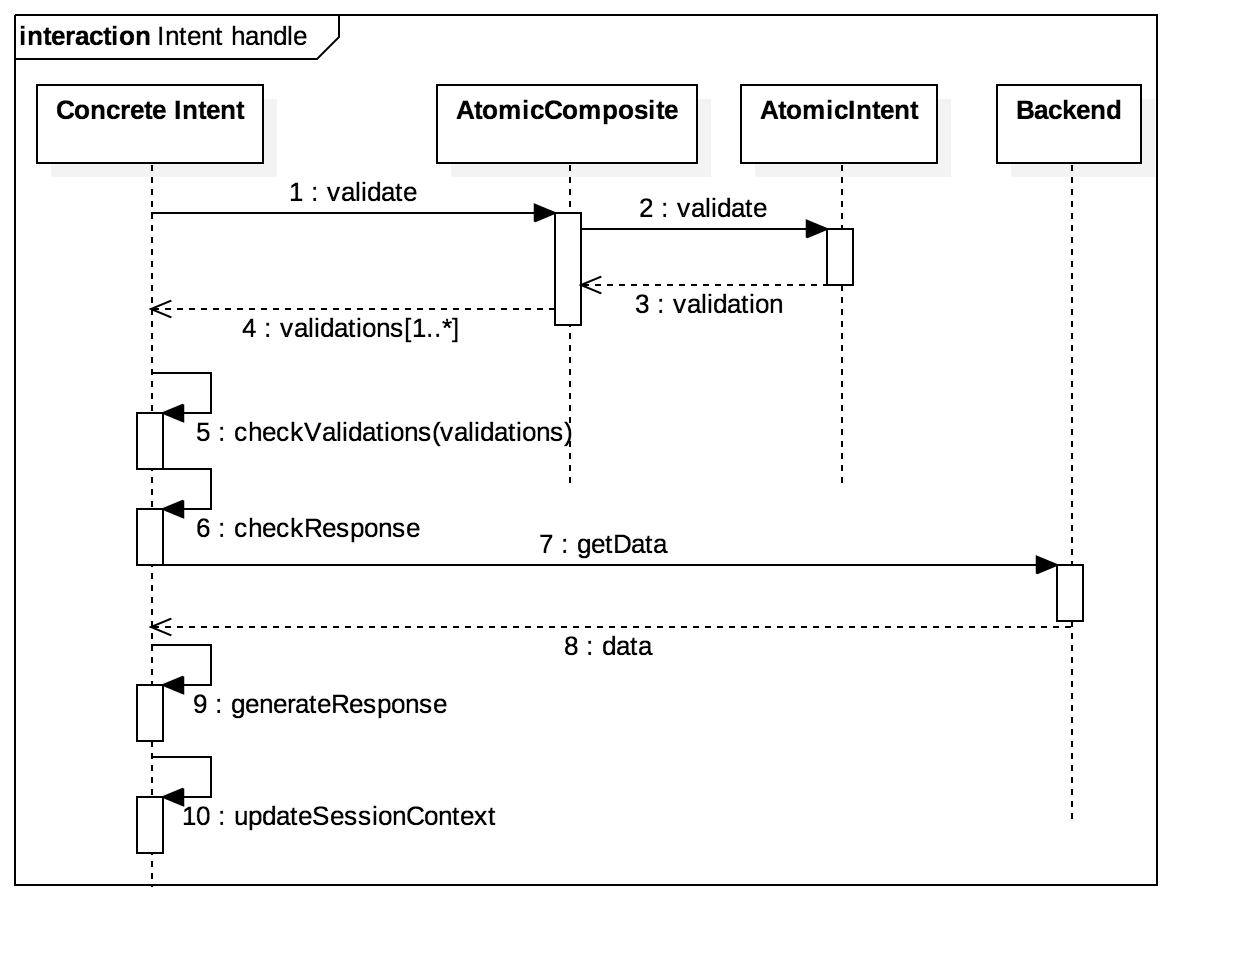
\includegraphics[width=1.0\textwidth]{bilder/4_skillSequenzIntentHandle.png}
    \caption{Sequenzdiagramm der Intent handle Funktion}
    \label{fig:skill-sequenz-handle}
\end{figure}

Die hier gegebenen Beschreibungen stellen die Prozesse der Architektur in allgemeiner Form dar. Im Folgenden werden daher die implementierten Intents mit ihren Besonderheiten zusammengefasst. 

\begin{itemize}
    \item Launch Intent: Der Launch Intent wird ausgeführt, wenn ein Benutzer den Skill startet und gibt lediglich eine der vordefinierten Antworten aus, um den Benutzer zu begrüßen. Dabei handelt es sich um einen Standard Intent, den jeder Skill implementieren muss
    
    \item Stop Intent: Mit dem Stop Intent verabschiedet sich der Skill vom Benutzer und beendet sich. Dieser Intent ist ebenfalls vorgeschrieben und muss von Skills implementiert werden.
    
    \item Help Intent: Auch die Hilfe muss implementiert werden. Sie gibt Beispielphrasen aus, die Nutzer für die Interaktion mit dem Skill verwenden können.
    
    \item User Intent: Der User Intent wird verwendet, um den Namen des Benutzers in Erfahrung zu bringen. Dabei handelt es sich um einen besonderen Intent. Er wird nicht vom Benutzer angestoßen, sondern in bestimmten Fällen vom Programm als Kontext im Session-Objekt gesetzt. Das ist notwendig, damit ein anschließend eingegebener Name auch als Benutzer Name für die Authentifizierung interpretiert werden kann. Ein Beispiel ist der Launch Intent. Nach Ausgabe des Willkommens Grußes, erfragt der Skill den Benutzer Namen. Ein weiteres Beispiel sind die Banking Funktionen. Ist der Benutzer bei Abfrage des Kontostandes noch nicht identifiziert, setzt der Skill den User Intent als Kontext und bittet den Benutzer  seinen Namen zu nennen. Nach Eingabe wird der Authentifizierungsmechanismus aus Abbildung \ref{fig:sequenz-authentifizierung} angestoßen.
    
    \item Authorise Intent: Ähnlich wie der User Intent, wird der Authorise Intent in bestimmten Situationen vom Programm initiiert. Er wird verwendet wenn ein bekannter, jedoch noch nicht authentifizierter Benutzer Banking Funktionen nutzen möchte. Über den Authorise Intent wird dann eine erneute Push-Nachricht an das Smartphone des Nutzers geschickt, damit dieser per Fingerabdruck bestätigt. 
    
    \item Balance Intent: Der Kontostand Intent enthält keine Slots. Wie im Authorise Intent beschrieben müssen Benutzer authentifiziert sein, bevor eine Abfrage des Kontostandes möglich ist. Natürlich muss der Benutzer vorher ein Konto über die App anbinden, um diese Funktion zu nutzen. Gemäß Abbildung \ref{fig:sequenz-kontostand} wird der Kontostand über das Backend und den Multibanking-Mock erfragt. 
    
    \item Transaction Intent: Die Transaktion ist der komplizierteste der implementierten Intents. Auch hier müssen zunächst Kriterien erfüllt werden. Ein Benutzer muss authentifiziert sein, ein Konto angebunden und Überweisungsvorlagen erstellt haben. Die Vorlage und der Betrag müssen vom Benutzer eingegeben werden. Bei fehlenden Slots gibt der Skill entsprechende Rückfragen aus. Ist die Validierung erfolgreich, wird die Überweisung zur Bestätigung noch einmal ausgegeben. Die Transaktion wird als Kontext gesetzt. Der Benutzer kann nun mit „ja“ bestätigen oder mit „nein“ ablehnen. Dabei handelt es sich auch um Atomic Intents. Ein „ja“ legt die Transaktion an. Der \ac{TAN} wird an das Smartphone des Benutzers gesendet. Im Anschluss setzt der Skill den \ac{TAN} Intent als Kontext. Bei einem „nein“ kann der der Benutzer die Slots noch einmal ändern oder andere Funktionen nutzen.
    
    \item \ac{TAN} Intent: Beim \ac{TAN} handelt es sich ebenfalls um einen vom Skill initiierten Intent. Nach Anlegen einer Transaktion wird dieser als Kontext gesetzt. Die an das Benutzer Smartphone übermittelte Nummer kann nun über Alexa eingegeben werden. Stimmt die Nummer überein, wird die Transaktion durchgeführt. Im Fehlerfall wird eine entsprechende Antwort ausgegeben.
\end{itemize}

An dieser Stelle sei erwähnt, dass der Kontext \bzw der aktuelle Intent jederzeit gewechselt werden kann. Auch wenn der Skill den Benutzer darum bittet die \ac{TAN} einer Überweisung einzugeben, kann dieser im nächsten Schritt den Hilfe- oder Kontostand Intent ansprechen. Mit dem entwickelten Prototypen ist es allerdings nicht möglich, im Anschluss zurück zum \ac{TAN} Intent zu wechseln. Auch wenn dies technisch möglich ist, kann es aus zeitlichen Gründen nicht im Zuge dieser Arbeit umgesetzt werden.\\
Damit Alexa die Daten entsprechend der Implementierung verstehen und an den Skill-Server senden kann, wird in Kapitel \ref{sec:interaction-model} das Interaction Model des Skills erstellt. Der Quelltext des Voice Bank Skill-Servers ist auf der beiliegenden CD unter \textit{„Quelltexte/finlexa\_skill/“} zu finden.

\section{Interaction Model}
\label{sec:interaction-model}
Damit Alexa die verwendeten Formulierungen für den Skill verstehen kann, muss man das Interaction Model erstellen. Hier werden die Intens, Slots und Utterances des Skills angegeben und miteinander verknüpft. Dabei wird das Konzept aus Kapitel \ref{sec:anhang-konzept} für die implementierten Intents verwendet. Des Weiteren sind hier der Skill und Invocation Name einzutragen.  Abbildung \ref{fig:interaction-model} zeigt den Abschnitt des Amazon Developer Portals, der für das Interaction Model des Voice Bank Skill zuständig ist. \newpage

\begin{figure}[!htb]
    \centering
    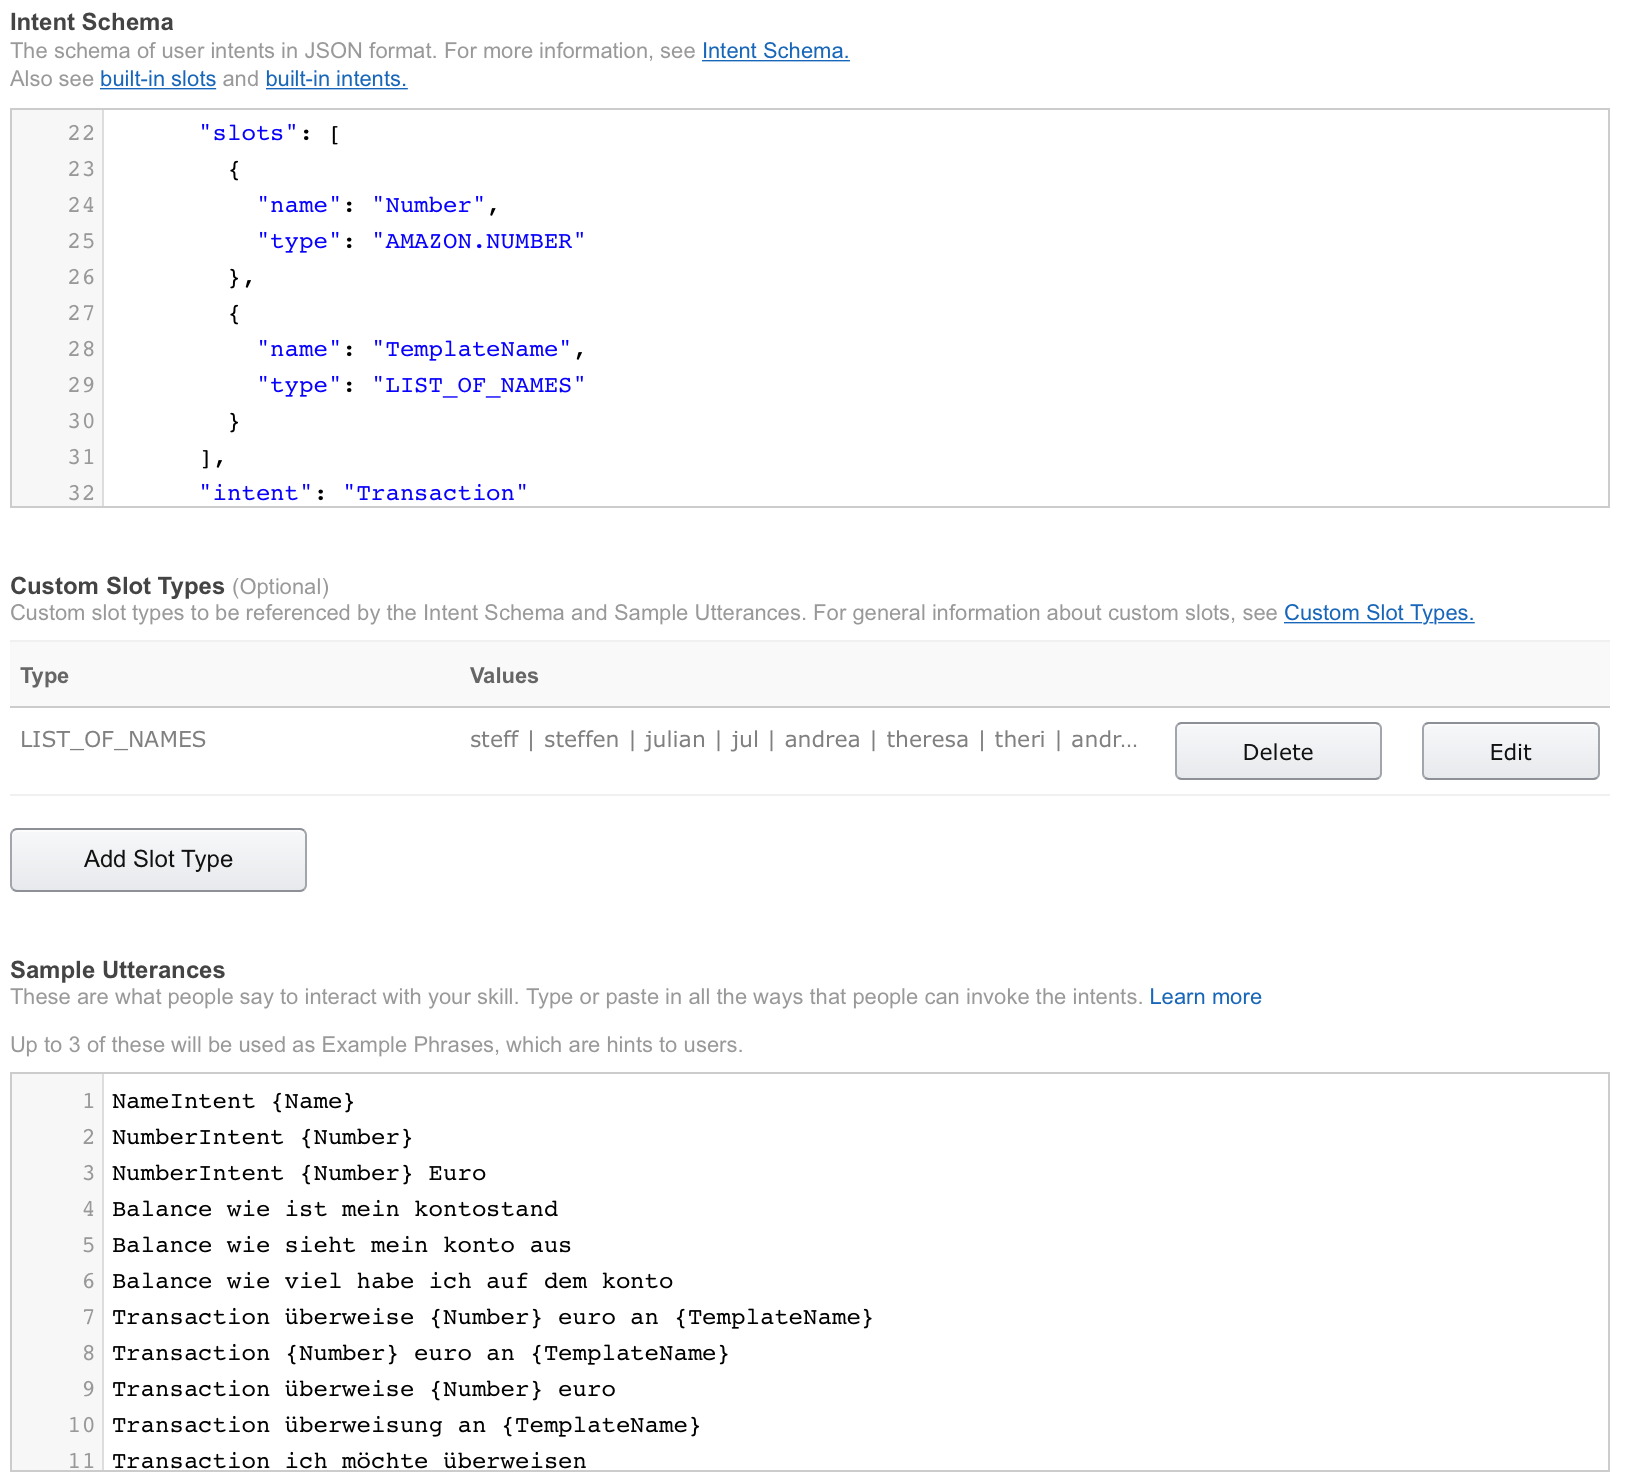
\includegraphics[width=1.0\textwidth]{bilder/4_interactionModel.png}
    \caption{Ausschnitt des Voice Bank Interaction Models}
    \label{fig:interaction-model}
\end{figure}

Dort sind das \textit{Intent Schema}, \textit{Custom Slot Values} und die Utterances zu sehen. Im Intent Schema wird zunächst jeder verwendete Intent mit etwaigen Slots in \ac{JSON} Form angegeben. Neben den Slot Namen ist hier auch der Typ festzulegen. Amazon unterstützt häufig verwendete Typen wie \zB \textit{AMAZON.Date}, \textit{AMAZON.Number} und \textit{AMAZON.Time} \cite{alexa-slot-types}. Diese ermöglichen, dass selbst unterschiedlich formulierte Eingaben eine einheitliche Ausgabe für den Skill-Server gewährleisten. Angaben zu einem bestimmten Tag, darunter „morgen“, „Dienstag“ oder „22.11.2017“, werden in Form von „YYYY-MM-DD“ ausgegeben, \zB 2017-11-22. Während Eingaben zu Wochen, wie „diese Woche“ und “nächste Woche“, als Kalenderwoche interpretiert werden \zB 2017-W47. Es ist auch möglich eigene Typen zu definieren. Das sind die Custom Slot Values aus Abbildung \ref{sec:interaction-model}. Im unteren Feld werden die Utterances nach dem bereits bekannten Schema (\vgl Kapitel \ref{subsec:skill-ask-sdk} und \ref{subsec:skill-architektur}) eingetragen. Abbildung \ref{sec:interaction-model} zeigt dabei nur einen Ausschnitt der definierten Formulierungen. Hier zu sehen sind die zwei Atomic Intents „Number“, “Name“ und ein Teil der „Kontostand“ und “Transaktion“ Intents. An dieser Stelle fließen auch die erarbeiteten Formulierungen aus dem Konzept mit ein. Sämtliche Utterances aus Abbildung \ref{fig:concept-transaction-name} und \ref{fig:concept-balance} werden ergänzt. Im nächsten Schritt ist die Adresse des Skill-Servers zu konfigurieren. Diese wird in Kapitel \ref{sec:deployment} eingefügt, da der Server zunächst bereitgestellt werden soll. Mit dem Anlegen dieses Skills im Developer Portal, der Angabe des Invocation \bzw Skill Namens, des Models und der Server Adresse kann der Skill bereits mit den Alexa Endgeräten des Entwicklers genutzt werden. Um den Skill in den Store hochzuladen, damit ihn auch andere Benutzer verwenden können, sind weitere Schritte nötig. Dabei müssen eine Beschreibung, Beispielphrasen für die Verwendung, ein Icon und weitere Angaben gemacht werden. Der Prozess der Skill Veröffentlichung wird im Zuge dieser Arbeit nicht beschrieben. Das Intent Schema und die Utterances des Interaction Models sind auf der CD unter \textit{„Quelltexte/finlexa\_model“} zu finden. Kapitel \ref{sec:deployment} zeigt den Vorgang und die verwendeten Technologien bei der Bereitstellung des Skill-Servers und Backends.

\section{Deployment}
\label{sec:deployment}
Der umgesetzte Prototyp wird nicht nur lokal über den Rechner gestartet. Der Skill-Server ist über das Web erreichbar. Dabei kommt nicht \ac{AWS}, sondern die Infrastruktur des Projektträgers zum Einsatz. Die dabei verwendeten Technologien werden im Folgenden kurz zusammengefasst.

\begin{itemize}
    \item \textit{Docker}: Docker ist eine offene Plattform zum Entwickeln, Ausliefern und Betreiben von verteilten Applikationen. Anwendungen sind in unabhängigen Containern organisiert. Anders als eine \ac{VM}, nutzen Docker Container das vorhandene Betriebssystem. Das spart Rechenleistung, da kein zusätzliches Betriebssystem emuliert werden muss. Über eine entsprechende Konfigurationsdatei kann mit Hilfe der Kommandozeile ein Abbild eines Containers generiert und gestartet werden. Diese können auch auf Server und Cloud Plattformen hochgeladen werden \cite{docker}. Listing \ref{lst:dockerfile} zeigt die Konfigurationsdatei, das sogenanntes \textit{dockerfile}, für den Skill-Server.\newpage
    
    \begin{lstlisting}[language={HTML},caption={Dockerfile des Voice Bank Skill-Servers},label={lst:dockerfile}]
    FROM node:boron

    ADD . /usr/src/app
    WORKDIR /usr/src/app
    
    RUN npm install -g tsc typescript
    
    RUN npm install
    
    RUN tsc 
    
    EXPOSE 3000
    CMD ["npm", "start"]

    \end{lstlisting}
    
    Dabei wird ein Basis Container „node:boron“ verwendet, der auf einem Linux Betriebssystem aufsetzt und bereits Node.js vorinstalliert hat. Im Anschluss werden die relevanten Quelltext Dateien (hier TypeScript Code) des Skill-Servers in die Ordnerstruktur der Linux Umgebung kopiert. Benötigte \ac{npm} Module müssen zunächst installiert werden. Im weiteren Verlauf wird der \ac{TS} Code kompiliert, der Port 3000 freigegeben und die Anwendung gestartet.
    
    \item \textit{OpenShift}: OpenShift ist eine open source Container Plattform. Sie basiert \ua auf Docker und ermöglicht das Verwalten, Betreiben und Warten von Docker Containern in Projekten. Ein Projekt kann dabei mehrere Container enthalten, die untereinander kommunizieren und von außen erreichbar sein können. Die OpenShift Umgebung wird vom Projektträger bereit gestellt. 
\end{itemize}

Skill-Server, Backend und die Datenbank sind jeweils in einem eigenen Docker Container organisiert. Die entsprechenden dockerfiles sind auf der CD im jeweiligen Ordner abgelegt. Das Dockerfile der Datenbank befindet sich unter \textit{„Quelltexte/finlexa\_central/database/“}. Diese Container werden in ein Projekt auf der OpenShift Plattform des Projektträgers hochgeladen. Abbildung \ref{fig:openshift} zeigt die Web Oberfläche dieses Projektes mit den drei laufenden Containern.\newpage

\begin{figure}[!htb]
    \centering
    \includegraphics[width=1.0\textwidth]{bilder/4_openshift.png}
    \caption{Voice Bank Projekt in OpenShift}
    \label{fig:openshift}
\end{figure}

Da der Name des Systems erst gegen Ende der Arbeit von „finlexa“ auf „Voice Bank“ geändert wurde, sind die Container hier mit dem alten Namen gekennzeichnet. Der „finlexa-central“ bildet das in der Umsetzung beschriebene Backend ab. Damit der Skill-Server und das Backend von außen erreichbar sind, werden für beide Routen angelegt. Die entsprechenden \acp{URL} sind in Abbildung \ref{fig:openshift} aus Sicherheitsgründen geschwärzt. Wird im Interaction Model die hier angelegte Route als Adresse des Skill-Servers eingegeben, hat Alexa Zugriff und der Skill kann über den Echo verwendet werden. Ebenso muss die Adresse des Backends in der Smartphone-App hinterlegt sein. Das folgende Kapitel \ref{sec:evaluierung} evaluiert die beschriebene Umsetzung des Prototypen.

\section{Evaluierung}
\label{sec:evaluierung}
Nach ersten Konversationen mit dem Skill Prototypen, wird klar, dass das kontextbasierte Verarbeiten der Intents, Komplettieren der Slots und die Authentifizierung den konzipierten Sequenzen folgen. Anhand dessen kann man darauf schließen, dass das Sicherheits-Konzept und die implementierte Architektur funktionieren. Es sei jedoch an dieser Stelle erwähnt, dass aufgrund der zeitlichen Begrenzung keine User Tests mit dem Prototypen durchgeführt werden können. Da die entwickelte App (Kapitel \ref{sec:app}) aus dem gleichen Grund eher funktional und weniger benutzerfreundlich umgesetzt ist, hat sie beim Test des Gesamtsystems womöglich negative Auswirkungen. Um zu beweisen, dass das System auch zufriedenstellend funktioniert und um eine fundierte Aussage treffen zu können, muss demnach die App entsprechend entwickelt und der Skill außerhalb dieser Arbeit getestet werden.\\ 
Die Implementierung der Architektur an sich ist anfangs zeitaufwändig. Jedoch ist zu bemerken, dass die Stärken vor allem bei zunehmender Komplexität ersichtlich werden. Hat man das Grundgerüst programmiert, lassen sich neue Intents \bzw Atomic Intents schnell hinzufügen. Aufgrund der Klassenhierarchie sind lediglich die Routinen der Valdierung \bzw handle Methode zu schreiben, die Intents in die entsprechende Fatory einzupflegen und die Antwortphrasen zu definieren. Das umgesetzte Sicherheits-Konzept zeigt außerdem, dass die Interaktion zwischen Alexa und der entwickelten App auch ohne Event-Unterstützung erfolgen kann. Es bietet die Möglichkeit Benutzer ohne Stimmenerkennung zu identifizieren. Jedoch ist die Nutzung des Mechanismus mit mehr Zeitaufwand für den Nutzer verbunden. Das folgende Kapitel \ref{cha:schlussbetrachtung} zieht ein Fazit der gesamten Arbeit und gibt einen Ausblick.


\chapter{Schlussbetrachtung}
\label{cha:schlussbetrachtung}
Im Folgenden wird die gesamte Arbeit rekapituliert und ein Ausblick gegeben.

\section{Fazit}
\label{sec:fazit}
Gegenstand der vorliegenden Arbeit war die Konzeptionierung und prototypische Umsetzung eines \ac{CUI} für das Bankkonten-Management. Unter Berücksichtigung der Gebrauchstauglichkeit und den sicherheitskritischen Aspekten des Nutzungskontextes war das Ziel zu untersuchen, welche der Anforderungen zufriedenstellend erfüllt werden können. Da es sich bei \acp{CUI} um eine natürliche Art der Interaktion handelt, lag der Fokus der Konzeption für sämtliche Schritte bei den potentiellen Benutzern.\\ 
Dabei ergab sich, dass nahezu jeder der Befragten große Skepsis gegenüber \acp{CUI} zum Ausdruck brachte, da für sie vor allem Sicherheit und Datenschutz ein zentrale Rolle einnahmen. Es wurde außerdem deutlich, dass es viele der einbezogenen Personen seltsam und unnatürlich fanden mit einer Maschine zu sprechen. Andererseits konnten die angewandten Methoden aus dem Usability Engineering zeigen, dass die Vorteile eines solchen Systems durchaus von potentiellen Nutzern erkannt wurden. Anhand dieser Befunde bestätigte sich die Entscheidung viel Zeit in die Anforderungsanalyse und benutzerorientierte Konzeption zu investieren, um das nötige Grundverständnis für die Nutzer und den Nutzungskontext zu schaffen. Die Durchführung der Interviews erzielte dabei nicht das gewünschte Ergebnis, da sie nur wenig neue Informationen ergaben. Es konnte jedoch darauf geschlossen werden, dass die Fehler bei der Ausführung der Grund für die mäßigen Ergebnisse waren und nicht die Entscheidung für diese Methode. Was das Prototyping betrifft, wurde ersichtlich, wie essenziell frühe Tests bei der Entwicklung von \acp{CUI} sind. Die erarbeitete Prototyping Toolchain trug maßgeblich zum Konzept des Skills bei, wie anhand der Ergebnisse deutlich wurde. Die Umsetzung des Prototyping Systems erfüllte die gestellten Anforderungen, mit der Einschränkung, dass aufgrund des fehlenden \ac{cft} Tools anfangs viel Zeit in die Vorbereitung der Tests floss. Mit der Umsetzung des Sicherheits-Konzeptes wurde eine Möglichkeit gezeigt wie man Benutzer von Alexa auch ohne Stimmenerkennung identifizieren kann, jedoch mit dem Kompromiss eines größeren Zeitaufwandes für den Benutzer. Was die Umsetzung des Skill-Servers betrifft wurde ersichtlich, dass die implementierte Architektur eine Alternative zum Alexa \ac{SDK} darstellt. Obwohl der Einstieg etwas schwieriger war, wurde eine Möglichkeit geschaffen Redundanzen in der Verarbeitung der Slots zu vermeiden und Alexa Requests kontextbasiert zu verarbeiten. Nach der Komplettierung und Bereitstellung des Systems, zeigten erste Tests, dass der Skill gemäß der konzipierten Prozesse arbeitet. Sowohl der Kontostand-, als auch der Transaktions-Intent konnten ausgeführt werden.\\
Somit wurden die Anforderungen teilweise erfüllt. Der Kontext konnte jederzeit gewechselt werden, da es keine festen Konversationsabläufe gibt. Ebenso war das Nachfragen von kontextrelevanten Informationen durch das System gegeben. Allerdings ist das Bewusstsein für den Kontext nur eingeschränkt vorhanden. Zwar wertete der Skill Anfragen kontextbasiert aus, jedoch werden vergangene Interaktionen nicht gespeichert. Nach einem Wechsel von einer fast abgeschlossenen Transaktion zum Kontostand konnte man nicht  zurückkehren, sondern musste die Transaktion erneut starten.\\ Über die Zufriedenstellung der umgesetzten Anforderungen kann im Zuge dieser Arbeit keine fundierte Aussage getroffen werden. Um dieser Frage nachzugehen, müssen die dafür benötigten Benutzertests mit dem entwickelten Skill abseits der Arbeit durchgeführt werden. Des Weiteren ist für zukünftige Projekte zu überlegen, ob man den Prozess der Konzeption umstellt. Da die Prototyping Tests den größeren Nutzen aufwiesen, könnte man weniger Zeit in die Anforderungsanalyse und dafür mehr in das Prototyping investieren. Vor allem die konzeptionellen Ergebnisse der Arbeit werden für weitere Projekte wiederverwendet und weiterentwickelt. Darunter auch die entstandene Prototyping Toolchain, die Skill-Server Architektur und das Sicherheits-Konzept.

\section{Ausblick}
\label{sec:ausblick}
Die dargestellten Ergebnisse ließen sich durch weitere Untersuchungen ergänzen. Die Prototyping Toolchain könnte dahingehend erweitert werden, dass sie auch für das Prototyping von textbasierten \acp{CUI} Verwendung findet. Des Weiteren ist die Entwicklung des cft-Tools denkbar, um die Anwendung zu erleichtern. Auch der Skill bietet viele Möglichkeiten für weiterführende Arbeiten, wie \zB den Ausbau der vorgestellten Architektur. Wird sie vom Bankkontext entkoppelt, wäre die Veröffentlichung einer eigenen Open-Source-Bibliothek denkbar, die das Grundgerüst und möglicherweise Atomic Intents für alle Arten von Slot Typen bereitstellt. Nicht nur für Alexa, sondern auch für andere \acp{VUI} könnten Anwendungen mit der gleichen Basis entwickelt werden.\\
Was die weitere Entwicklung der \acp{CUI} im Allgemeinen betrifft, wird abschließend auf einen Absatz aus der Literatur verwiesen:
\begin{quote}
It has been predicted in a number of studies that the global market for VPAs will increase dramatically in the next few years. One factor in addition to those discussed above is the so-called cycle of increasing returns. User acceptance and adoption interact with developments in technology to produce a cycle of increasing returns. As performance improves, more people will use conversational interfaces. With more usage, there will be more data that the systems can use to learn and improve. And the more they improve, the more people will want to use them. Given this cycle, it can be expected that conversational interfaces will see a large uptake for some time to come and that this uptake will be accompanied by enhanced functionalities and performance \cite{mctear-cui}. 
\end{quote}

\csappto{theglossary}{\label{cha:glossar}}
\printglossaries

\small
\bibliographystyle{literatur/myalpha}
\bibliography{literatur/Bibliographie}
\normalsize

\begin{appendix}
    \clearpage
    \pagenumbering{roman}
    \chapter{Anhang}
    \label{sec:Anhang}
    % Rand der Aufzählungen in Tabellen anpassen
    \setdefaultleftmargin{1em}{}{}{}{}{}
    \section{Ausführung Online Umfrage}
\label{sec:ausfuehrung-online-umfrage}
Im Folgenden werden die Fragen und Antworten der Online Umfrage ausführlich dargestellt. Die Durchführung und Ergebnisse sind in Kapitel \ref{subsec:online-umfrage} zusammengefasst.

\begin{enumerate}
    \item \textbf{Verwenden Sie Online Banking?} \\ Anzahl Teilnehmer: 48
    \begin{itemize}
        \item[] 44 (91.7\%): ja
        \item[] 4 (8.3\%): nein
    \end{itemize}
    
    \item \textbf{Was müsste sich ändern, damit Sie es verwenden würden?}\\ Anzahl Teilnehmer: 3
    \begin{itemize}
        \item[] Nichts
        \item[] Sicherheitsproblematik
        \item[] Wenn mir jemand beim Einrichten hilft, würde ich es sofort verwenden
    \end{itemize}
    
    \item \textbf{Was sind Ihre Hauptgründe für die Nutzung von Online Banking?}\\ Anzahl Teilnehmer: 44
    \begin{itemize}
        \item[] 16 (36.4\%): Öffnungszeiten der Banken
        \item[] 36 (81.8\%): Schnell
        \item[] 10 (22.7\%): Kostengünstig
        \item[] 23 (52.3\%): Überall Zugriff
        \item[] 34 (77.3\%): Bequem
        \item[] 0 (0.0\%): Andere
    \end{itemize}
    
     \item \textbf{Aus welchen konkreten Gründen prüfen Sie Ihren Kontostand bzw. Ihre Umsatzanzeige?}\\ Anzahl Teilnehmer: 44
     \begin{itemize}
        \item Abbuchungen
        \item Aktuelles Guthaben
        \item Kontrolle
        \item Aktualität: Was ist drauf was wird abgebucht was kann ich mir noch leisten
        \item Kontrolle
        \item Um auf dem aktuellen Stand zu sein
        \item Um zu prüfen
        \item Zur Überwachung
        \item Um zu sehen ob alles richtig läuft
        \item Damit man die Kosten immer im Auge hat
        \item Übersicht
        \item Kontostand
        \item Allgemeiner Überblick vor Überweisungen
        \item Um immer zu wissen wie viel Geld man hat und um den Cashflow im Auge zu haben
        \item Kontrolle
        \item Damit ich weiß, wieviel Geld noch auf dem Konto ist bzw. ob Auffälligkeiten sind
        \item Ob alle Daueraufträge korrekt sind und nichts falsch abgebucht wird
        \item Fehlbuchungen Kontrolle über Ausgaben
        \item damit nicht unbefugtes abgebucht wird
        \item ob Lohn da ist
        \item ob ich evtl. Geld aus Gutschriften etc. erhalten hab
        \item Um auf dem Laufenden über meinen Kontostatus zu haben
        \item Zahlungs ein-/ausgabekontrolle von onlineshopping
        \item Papier sparen
        \item Vermeidung von Missbrauch und einfache Übersicht
        \item Kontrolle zu Ein und Ausgaben
        \item Übersicht Barvermögen, Lastschriften überwachen
        \item Um den Kontostand zu erfahren und über den Zahlungsverkehr auf dem Laufenden zu sein
        \item Sicherheit
        \item Den aktuelle Kontostand im Blick haben
        \item Um zu sehen wie viel Geld auf dem Konto ist
        \item Um Überblick auf alle Transaktionen zu haben
        \item Um nicht ins Minus zu rutschen
        \item Sind die Abbuchungen erlaubt
        \item Sind Einnahmen überwiesen
        \item Um falsche Abbuchungen zu vermeiden Den Kontostand im Blick zu haben
        \item Prüfung von Fehlbuchungen
    \end{itemize}
    
     \item \textbf{Führen Sie mit Online Banking Überweisungen durch?} \\ Anzahl Teilnehmer: 44
    \begin{itemize}
        \item[] 44 (100\%): ja
        \item[] 0 (0\%): nein
    \end{itemize}
    
     \item \textbf{In welcher Form führen Sie Überweisungen durch? (mehrere Antworten möglich)} \\ Anzahl Teilnehmer: 44
    \begin{itemize}
        \item[] 22 (50.0\%): Unter Verwendung von Überweisungsvorlagen
        \item[] 37 (84.1\%): Überweisungsformular ausfüllen
        \item[] 27 (61.4\%): Daueraufträge einrichten
    \end{itemize}
    
     \item \textbf{Welches TAN Verfahren verwenden Sie dabei?} \\ Anzahl Teilnehmer: 44
    \begin{itemize}
        \item[] 1 (2.3\%): iTAN (Liste)
        \item[] 20 (45.5\%): mTAN (SMS)
        \item[] 17 (38.6\%): smartTAN (EC Kartenleser)
        \item[] 4 (9.1\%): pushTAN (Smartphone App)
        \item[] 2 (4.5\%): Andere 
        \item[] Antworten aus dem Zusatzfeld: 
        \begin{itemize}
            \item[] Chip Tan
            \item[] Sowohl mtan und pushTAN
        \end{itemize}
    \end{itemize}
    
    \item \textbf{Nutzen Sie ein Finanzmanagement- System, um Ihre Kontodaten über längere Zeiträume auszuwerten?} \\ Anzahl Teilnehmer: 44
    \begin{itemize}
        \item[] 9 (20.5\%): ja
        \item[] 35 (79.5\%): nein
    \end{itemize}
    
    \item \textbf{Welche Funktionen verwenden Sie dabei? (mehrere Antworten möglich)} \\ Anzahl Teilnehmer: 9
    \begin{itemize}
        \item[] 2 (22.2\%): Anlegen und Verwalten von Sparzielen/Budgets
        \item[] 8 (88.9\%): Auswertung Ihrer Umsätze
        \item[] 0 (0.0\%): Andere
    \end{itemize}
    
     \item \textbf{Investieren Sie in Aktien?} \\ Anzahl Teilnehmer: 44
    \begin{itemize}
        \item[] 9 (20.5\%): ja
        \item[] 35 (79.5\%): nein
    \end{itemize}
    
    \item \textbf{Verwenden Sie ein Online Portal für die Verwaltung Ihrer Aktien?} \\ Anzahl Teilnehmer: 10
    \begin{itemize}
        \item[] 4 (40.0\%): ja
        \item[] 6 (60.0\%): nein
    \end{itemize}
    
     \item \textbf{Nach welchen Kriterien wählen Sie neue AKtien aus?}\\ Anzahl Teilnehmer: 8
     \begin{itemize}
        \item nach der Rendite unter Berücksichtigung des Risikos
        \item o.A.
        \item Risiko
        \item Aktien, die neu auf den Markt kommen
        \item Aktien die hohe Dividende bieten
        \item Aktien von weltbekannten Firmen wie z.B. Siemens, Coca Cola, etc.
        \item Kgv
        \item Nach Analyse von mir selbst
        \item Broker Informationen
        \item Blue Chips
        \item Branchenmix
    \end{itemize}
    
    \item \textbf{Welche Informationen Ihrer Aktien rufen Sie regelmäßig ab?}\\ Anzahl Teilnehmer: 8
     \begin{itemize}
        \item Kosten und Gewinn
        \item o.A.
        \item Sicherheit und Transparenz
        \item aktuelle Kurse
        \item Höchst und Niedrigkurs der letzten 12 Monate
        \item Kurs Chart der letzten fünf Jahre
        \item Kurs
        \item News der investierten Aktien
        \item Aktueller Stand
        \item Kurs
        \item Wirtschaftspresse
        \item Online Informationen
    \end{itemize}
    
     \item \textbf{Haben Sie bei der Nutzung von Online Banking sicherheitsrelevante Bedenken? Wenn ja welche? (mehrere Antworten möglich)} \\ Anzahl Teilnehmer: 43
    \begin{itemize}
        \item[] 22 (51.2\%): Account Sicherheit
        \item[] 2 (4.7\%): Cookies
        \item[] 30 (69.8\%): Hacker
        \item[] 11 (25.6\%): Identitätsraub
        \item[] 6 (14.0\%): Internet Verbindung
        \item[] 10 (23.3\%): Keine Bedenken
        \item[] 0 (0.0\%): Andere 
    \end{itemize}
    
     \item \textbf{Wie könnte Online Banking für Sie effizienter ablaufen?}\\ Anzahl Teilnehmer: 43
     \begin{itemize}
        \item Kartenleser schlecht abzulesen
        \item Keine Ahnung
        \item Für solche Fragen gibt es Leute wie dich hehe
        \item Es ist effizient genug
        \item Gar nicht. Hacker Probleme wird es immer geben...
        \item noch effizienter?
        \item Prinzipiell läuft es gut, nur werden Anwendungen schon angeboten, die teilweise noch nicht ganz ausgereift sind (z.B. Rechnungsscan)
        \item Keine Ahnung
        \item ?
        \item Ist i.O.!
        \item Mehrere Unterkonten in einem Konto, um das Geld für verschiedene Themen aufzuteilen (z.B. Lebensmittel, Versicherungen, sparen usw.)
        \item Keine Ahnung
        \item Bin bisher zufrieden
        \item Keine Ideen und Vorschläge
        \item Für mich ist es schon effizient
        \item Durch Fingerabdruck/Augenscan anstatt Password beim Login
        \item Sicherheit und gleichzeitig Handling verbessern
        \item ist effizient genug
        \item Deutliche Qualitäts- und Sicherheitssteigerung in Apps
        \item Schnellere aktualisierung der Kontostände
        \item eventuell Benachrichtigung bei ankommenden/abgehenden Geld per app
        \item USB Kartenleser um das umständliche halten des EC Kartenlesers zu vermeiden
        \item Schnellere Auswertung vom TAN Generator
        \item Weiß nicht
        \item aktuelle keine Verbesserung am Onlinebanking - Verfahren notwendig
        \item Aktuell bin ich zufrieden
        \item Zugriffe auch für alle Sparbücher, Konten usw.
        \item Könnte schneller sein die Formulare auszufüllen
        \item Überweisungen über Handy app mit digitale überweisungsformular so dass man nur noch bestätigen muss. Gleichzeitig MUSS das System 1000\% sicher sein.
        \item Depotdaten sollten besser ausgewertet sein
        \item Stärkere Verzahnung des Online-Auftritts mit dem persönlichen Kontakt in der Filiale (\zB Terminvereinbarungen, ToDos aus den Termin tracken etc.)
    \end{itemize}
    
    \item \textbf{Wie alt sind Sie?} \\ Anzahl Teilnehmer: 43
    \begin{itemize}
        \item[] 0 (0.0\%): unter 18 Jahre
        \item[] 20 (46.5\%): 18 - 30 Jahre
        \item[] 12 (27.9\%): 31 - 40 Jahre
        \item[] 6 (14.0\%): 41 - 50 Jahre
        \item[] 4 (9.3\%): 51 - 60 Jahre
        \item[] 1 (2.3\%): über 60 Jahre
    \end{itemize}
\end{enumerate}

\section{Interview Einverständniserklärung}
\label{sec:ausfuehrung-interview-einverstaendnis}
Die folgende Einverständniserklärung wird den Teilnehmern vor der Durchführung des Interviews zur Unterschrift vorgelegt. Die Durchführung der Interviews ist in Kapitel \ref{subsec:interviews} genauer beschrieben. \\

\textbf{Einverständniserklärung zum Interview}\\

Forschungsprojekt: Sprachassistenzsysteme im Bankkontenmanagement\\
Durchführende Institution: \adorsys \\
Projektleitung: Steffen Blümm\\
Interviewerin/Interviewer: Julian Wölk\\
Interviewdatum:\\\\
Ich erkläre mich dazu bereit, im Rahmen des genannten Forschungsprojekts an einem Interview teilzunehmen. Ich wurde über das Ziel und den Verlauf des Forschungsprojekts informiert. Ich kann das Interview jederzeit abbrechen, weitere Interviews ablehnen und meine Einwilligung in eine Aufzeichnung und Niederschrift des/der Interviews zurückziehen, ohne dass mir dadurch irgendwelche Nachteile entstehen.\\
Ich bin damit einverstanden, dass das Interview mit einem Aufnahmegerät aufgezeichnet und sodann von den Mitarbeiterinnen und Mitarbeitern des Studienprojekts in Schriftform gebracht wird. Für die weitere wissenschaftliche Auswertung des Interviewtextes werden alle Angaben zu meiner Person aus dem Text entfernt und/oder anonymisiert. Mir wird außerdem versichert, dass das Interview in wissenschaftlichen Veröffentlichungen nur in Ausschnitten zitiert wird, um sicherzustellen, dass ich auch durch die in den Interviews erzählte Reihenfolge von Ereignissen nicht für Dritte erkennbar werde.

\vspace{3cm}

Ort, Datum, Unterschrift


\section{Interview Fragebogen}
\label{sec:ausfuehrung-interview-fragebogen}
Folgende Fragen werden den Interview Teilnehmern gestellt. Weitere Informationen zur Durchführung sind in Kapitel \ref{subsec:interviews}.

\begin{enumerate}
    \item Wie alt sind Sie?
    \item Wie ist Ihre Haltung zu Sprachassistenten?
    \item Hatten Sie bereits mit Sprachassistenten zu tun?
    \begin{enumerate}
        \item Wofür haben Sie diese verwendet?
        \item Was finden Sie positiv an Sprachassistenten?
        \item Was hat Ihnen bei der Nutzung nicht gefallen?
    \end{enumerate}
    \item Wie greifen Sie auf Ihr Bankkonto hauptsächlich zu?
    \item Wenn Sie Ihren Kontostand bzw. Ihre Umsatzanzeige prüfen, welche Intention haben Sie dabei?
    \item Wenn Sie Sprachassistenten in Verbindung mit Online Bankkonten Management hören, was kommt Ihnen dabei in den Sinn?
    \item Wie sieht Ihr Umfeld aus, wenn Sie auf Ihr Bankkonto zugreifen?
    \item Suche nach Formulierungen
    \begin{enumerate}
        \item Was würden Sie ein Bankkonto fragen?
        \item Wie würden sie nach dem Folgenden Fragen:
        \begin{enumerate}
            \item Kontostand
            \item Verdeckter Ausgabe des Kontostandes
            \item Gehaltseingang
            \item Spezielle Umsätzen
            \item Budget/Fixkosten
            \item Sparziel anlegen
            \item An Sparziel überweisen
            \item Sparziel Status
        \end{enumerate}
        \item Fällt Ihnen sonst noch etwas ein?
    \end{enumerate}
    \item Wie ist Ihre Meinung zu so einem System?
    \item Würden Sie ein solches System verwenden?
    \item Welche Bedenken hätten Sie?
    \item Fällt Ihnen sonst noch etwas zu dem Thema ein?
\end{enumerate}

\section{Interview Auswertung}
\label{sec:ausfuehrung-interview-auswertung}
Die schriftliche Auswertung der Interviews ist stichpunktartig und sinngemäß unter Verwendung eigener Worte dokumentiert. Damit, wie in der Einverständniserklärung aus \ref{sec:ausfuehrung-interview-einverstaendnis} vereinbart, keine Rückschlüsse auf die Teilnehmer gezogen werden können, ist zudem die Anordnung der Antworten zufällig gewählt und entspricht keinem chronologischen Muster. 

\begin{enumerate}
    \item Altersgruppe 22 - 26
    \item Meinungen zu Sprachassistenten
    \begin{itemize}
        \item Eher skeptisch
        \item Cool wenn es funktioniert
        \item Missbrauch von Daten hat man nicht im Griff
        \item Grundsätzlich gut und praktisch, wenn es anständig funktioniert
        \item Erspart Tipparbeit
        \item Befremdlich
        \item Erleichtert vieles
        \item Es ist cool, mit Maschinen zu sprechen
    \end{itemize}
    \item Nur ein Teilnehmer hat Sprachassistenten bereits genutzt (Suchanfragen über Smartphone)
    \item Zugriff auf Bankkonto
    \begin{itemize}
        \item Erfolgt bei allen Teilnehmern über Online Banking am Rechner
        \item In Ausnahmesituationen auch über Smartphone (zum Beispiel Urlaub)
        \item Weg zur Bank nur bei Einzahlungen
    \end{itemize}
    \item Intentionen beim Prüfen von Kontostand und Umsatzdaten
    \begin{itemize}
        \item Überprüfen/Überwachen
        \item Ein- und Ausgang von Transaktionen prüfen
        \item Telefon Rechnung Mitte des Monats prüfen
        \item Gehaltseingang prüfen
        \item Kontoübersicht
        \item Prüfen des Guthabens vor dem Kauf bestimmter Dinge
        \item Stand am Monatsende prüfen
        \item Umssatzdaten speichern
    \end{itemize}
    \item Meinungen zu Sprachassistent in Verbindung mit Bankkonten Management
    \begin{itemize}
        \item Überwiegend Sicherheitsbedenken
        \item Angst vor Stimmen Fälschung, Missbrauch
        \item Vereinfachte Umsatzabfragen
        \item Schneller Zugriff auf Informationen
        \item Erspart Tipp- und Klickarbeit
        \item Praktisch
        \item Vorsicht bei Nutzung neuer Technologien
    \end{itemize}
    \item Teilnehmer sind während Ihrer Online Banking Tätigkeiten überwiegend alleine
    \item Szenarien für das Finden von Formulierungen
    \begin{enumerate}
        \item Kontostand
        \begin{itemize}
            \item Kontostand verdeckt ausgeben
            \item Wie ist mein Kontostand?
            \item Wie schaut mein aktueller Kontostand aus?
        \end{itemize}
        \item Gehaltseingang
        \begin{itemize}
            \item Ist das Gehalt eingegangen
            \item Zeig mir die eingegangenen Gehälter von Firma X
        \end{itemize}
        \item Spezielle Umsätzen
        \begin{itemize}
            \item Hat Kontoinhaber/Firma X schon abgebucht?
            \item Was sind die ein und ausgegangenen Buchungen?
            \item Wurde schon die Überweisung von gestern abgebucht?
        \end{itemize}
        \item Budget/Fixkosten
        \begin{itemize}
            \item Wie sieht mein Konto aus?
        \end{itemize}
        \item Sparziel anlegen
        \begin{itemize}
            \item Lege mir ein neues Sparziel namens X fest, mit monatlich Y Euro, für ein Jahr
        \end{itemize}
    \end{enumerate}
    \item Meinungen zum System aus dem Szenario
    \begin{itemize}
        \item Skeptisch
        \item Sicherheitsproblematik
        \item Sinnvoll für einfache Fragen
        \item Zeitersparnis bei Transaktionen fraglich, da Spracheingabe einer IBAN, vor allem bei Eingabefehlern 
        \item Überweisungen lieber über Online Banking, da bessere Kontrolle
    \end{itemize}
    \item Frage, ob Teilnehmer so etwas verwenden würden
    \begin{itemize}
        \item Nur privat, nicht in der Öffentlichkeit
        \item Nur für Abfragen und nicht für Überweisungen
        \item Falls Zeitersparnis, eventuell ja
        \item Kommt auf die Bewertung der Benutzer an
    \end{itemize}
    \item Sonstige Ideen, Anmerkungen und Wünsche
    \begin{itemize}
    \item Bereitstellung von Informationen wie: 
    \begin{itemize}
        \item Wie wird der Datenschutz gehandhabt und gewährleistet
        \item Datenübertragung
        \item Verwendete Sicherheitsstandards
        \item Übertragungswege
    \end{itemize}
    \item Kostenlose Bereitstellung der Software
    \item Automatische Kategorisierung der Umsatzdaten
    \item Schneller Überblick zur Kontosituation
    \item Eingabefehler melden
    \item Beim Überziehen des Kontos warnen, ggf. einstellbar ob und wie gewarnt wird
    \item Anbindung des Kreditkarten-Kontos
    \item Benachrichtigung wenn etwas gebucht wurde
    \item Überweisungen wiederholen und bestätigen lassen, bevor diese abgeschickt werden
    \item Ein Banking System soll nicht duzen, das ist zu unseriös
    \end{itemize}
\end{enumerate}

\section{Liste aller Personas}
\label{sec:anhang-personas}
Im Folgenden werden alle der in Kapitel \ref{subsec:personas} modellierten Personas abgebildet. 

\begin{figure}[!htb]
    \centering
    \fbox{\includegraphics[width=1.0\textwidth]{bilder/3_alenaMeier.png}}
    \caption{Persona Alena Meier}
    \label{fig:alena-meier-anhang}
\end{figure}

\begin{figure}[!htb]
    \centering
    \fbox{\includegraphics[width=1.0\textwidth]{bilder/3_josefLech.png}}
    \caption{Persona Josef Lech}
    \label{fig:josef-lech}
\end{figure}

\begin{figure}[!htb]
    \centering
    \fbox{\includegraphics[width=1.0\textwidth]{bilder/3_robertTrier.png}}
    \caption{Persona Robert Trier}
    \label{fig:robert-trier}
\end{figure}

\begin{figure}[!htb]
    \centering
    \fbox{\includegraphics[width=1.0\textwidth]{bilder/3_danielaFriedmann.png}}
    \caption{Persona Daniela Friedmann}
    \label{fig:daniela-friedmann}
\end{figure}

\section{Liste der User Stories}
\label{sec:anhang-user-stories}
Im Folgenden sind alle identifizierten User Stories und etwaige Akzeptanzkriterien aufgeführt. Aus Platz- und Übersichtlichkeitsgründen stellen diese nur den aktuellen Stand dar. Die initiale Version aus Kapitel \ref{subsec:user-stories} und etwaige Zwischenstände sind hier nicht dokumentiert. Änderungen sind mit Referenz auf die Story in den jeweiligen Kapiteln genauer beschrieben.

\begin{enumerate}
\item\textbf{Hilfe aufrufen}: Als allgemeiner Benutzer, möchte ich mir Hilfestellung ausgeben lassen, um in Erfahrung zu bringen, welche Funktionen der Anwendung ich mit welchen Formulierungen verwenden kann.

\item\textbf{Profil anlegen}: Als allgemeiner Benutzer, möchte ich ein Profil anlegen, um für die Nutzung der Anwendung zu registrieren.

\item\textbf{Profil bearbeiten}: Als authentifizierter Benutzer, möchte ich mein Profil bearbeiten, um Änderungen daran vorzunehmen.

\item\textbf{Profil löschen}: Als authentifizierter Benutzer, möchte ich mein Profil löschen, um die Nutzung der Anwendung über dieses Profil einzustellen.

\item\textbf{Authentifizierung durchführen}: Als registrierter Benutzer, möchte ich mich authentifizieren, um den vollen Funktionsumfang der Anwendung nutzen zu können.

\item\textbf{Bankkonto anbinden}: Als authentifizierter Benutzer, möchte ich beliebige Bankkonten mit dem System verknüpfen, um diese mit der Anwendung verwalten zu können.

\item\textbf{Bankkonto-Verknüpfung bearbeiten}: Als authentifizierter Benutzer, möchte ich Bankkonten-Verknüpfungen bearbeiten, um den Namen der Konten zu ändern.

\item\textbf{Bankkonto-Verknüpfung löschen}: Als authentifizierter Benutzer, möchte ich Bankkonten-Verknüpfungen löschen, um die Anbindung für dieses Konto aufzuheben.

\item\textbf{Hauptkonto wählen}: Als authentifizierter Benutzer, möchte ich eines meiner Konten als Hauptkonto setzen, um Transaktionen und Berechnungen automatisch von diesem Konto aus ausführen zu lassen.

\item\textbf{Vorlagen anlegen}: Als authentifizierter Benutzer, möchte ich beliebig viele Überweisungs-Vorlagen anlegen, um Transaktionen durchführen zu können.

\item\textbf{Vorlagen bearbeiten}: Als authentifizierter Benutzer, möchte ich Überweisungs-Vorlagen bearbeiten, um Änderungen daran vorzunehmen.

\item\textbf{Vorlagen löschen}: Als authentifizierter Benutzer, möchte ich Überweisungs-Vorlagen löschen, um die Verwendung nicht genutzter Vorlagen einzustellen.

\item\textbf{Kontostand abfragen}: Als authentifizierter Benutzer, möchte ich den Kontostand abfragen, um herauszufinden wie viel Geld ich aktuell auf dem Konto habe.

\item\textbf{Transaktion via Vorlage tätigen}: Als authentifizierter Benutzer, möchte ich mit Hilfe der Überweisungsvorlagen Transaktionen durchführen, um schnell Geld an den in der Vorlage definierten Kontoinhaber zu überweisen.

\item\textbf{Transaktion via IBAN tätigen}: Als authentifizierter Benutzer, möchte ich mit Hilfe einer IBAN Transaktionen durchführen, um Geld an den Kontoinhaber dieser IBAN zu überweisen.

\item\textbf{TAN eingeben}: als authentifizierter Benutzer, möchte ich die die TAN Nummer für eine getätigte Transaktion eingeben, um diese Transaktion zu bestätigen.

\item\textbf{Gehaltseingang prüfen}: Als authentifizierter Benutzer, möchte ich ich prüfen, ob mein Gehalt überwiesen wurde, um dessen Eingang schnell und ohne Nennung der Höhe des Betrages abzufragen.

\item\textbf{Höhe des Gehaltes prüfen}: Als authentifizierter Benutzer, möchte ich ich abrufen, wie hoch mein Gehalt ist, um zu prüfen, ob es korrekt verrechnet wurde.

\item\textbf{Datum des Gehaltes prüfen}: Als authentifizierter Benutzer, möchte ich ich abrufen, wann mein Gehalt überwiesen wurde, um zu prüfen, ob mein Arbeitgeber rechtzeitig überwiesen hat.

\item\textbf{Budget abrufen}: Als authentifizierter Benutzer, möchte ich wissen wie viel Geld ich bis Ende der aktuellen Finanzperiode zur Verfügung habe, um mein Ausgabeverhalten entsprechend anpassen zu können.

\item\textbf{Budget von letztem Monat abrufen}: Als authentifizierter Benutzer, möchte ich wissen wie viel Geld ich bis Ende des letzten Monates hatte, um zu prüfen, ob Änderungen in meinem Ausgabeverhalten Wirkung zeigen.

\item\textbf{Fixkosten prüfen}: Als authentifizierter Benutzer, möchte ich die Höhe und Art meiner Fixkosten wissen, um in Erfahrung zu bringen wofür ich regelmäßig wieviel Geld ausgebe.

\item\textbf{Umsatzdaten prüfen}: Als authentifizierter Benutzer, möchte ich Informationen zu Umsatzdaten abfragen, um in Erfahrung zu bringen, ob bestimmte Transaktionen durchgeführt wurden.

\item\textbf{Sparziele anlegen}: Als authentifizierter Benutzer, möchte ich auf verknüpften Sparkonten Sparziele anlegen, um für ein von mir festgelegtes Thema Geld zu sparen.

\item\textbf{Sparziele bearbeiten}: Als authentifizierter Benutzer, möchte ich Betrag, Intervall und Name von angelegten Sparzielen bearbeiten, um diese auf meine aktuellen Bedürfnisse anzupassen.

\item\textbf{Sparziele löschen}: Als authentifizierter Benutzer, möchte ich angelegte Sparziele löschen, um die Sparmaßnahmen für dieses Ziel einzustellen.

\item\textbf{Sparziele ausgeben}: Als authentifizierter Benutzer, möchte ich angelegte Sparziele ausgeben lassen, um in Erfahrung zu bringen, wofür ich bisher spare.

\item\textbf{Ausgaben der letzten Finanzperiode}: Als authentifizierter Benutzer möchte ich wissen, wie viel Geld ich in der letzten Finanzperiode insgesamt ausgegeben habe, um mein Ausgabeverhalten im Blick zu haben.
\end{enumerate}

\section{Liste aller Szenarien}
\label{sec:anhang-szenarien}
Im Folgenden werden alle entwickelten Szenarien aus Kapitel \ref{subsec:szenarien} dargestellt. 

\begin{figure}[!htb]
    \centering
    \fbox{\includegraphics[width=1.0\textwidth]{bilder/3_szenarioStudent.png}}
    \caption{Studenten Szenario}
    \label{fig:szenario-student}
\end{figure}

\begin{figure}[!htb]
    \centering
    \fbox{\includegraphics[width=1.0\textwidth]{bilder/3_szenarioPartner.png}}
    \caption{Partnerschaft Szenario}
    \label{fig:szenario-partner-anhang}
\end{figure}

\begin{figure}[!htb]
    \centering
    \fbox{\includegraphics[width=1.0\textwidth]{bilder/3_szenarioVerheiratet.png}}
    \caption{Verheiratet Szenario}
    \label{fig:szenario-verheiratet}
\end{figure}

\section{Communication Prototyping Tool Skript Schema}
\label{sec:cpt-input-schema}

Im Folgenden ist das Schema des Skriptes defniert, das vom CPT Tool für den Aufbau der Oberfläche verwendet wird.

\lstinputlisting[caption={Skript Schema der cft Ausgabe}]{docs/conversationPrototypingDocument.cft.json}

\section{Konzept}
\label{sec:anhang-konzept}
Die folgenden Abbildungen zeigen die ausgearbeiteten Intents und bilden das Bedienkonzept. Sie sind das Ergebnis der empirischen Daten und User Tests. Diese bilden die Basis für die Implementierung in Kapitel \ref{cha:umsetzung}.

\begin{figure}[!htb]
    \centering
    \fbox{\includegraphics[width=1.0\textwidth]{bilder/3_conceptBalance.png}}
    \caption{Kontostand Intent}
    \label{fig:concept-balance}
\end{figure}

\begin{figure}[!htb]
    \centering
    \fbox{\includegraphics[width=1.0\textwidth]{bilder/3_conceptBudget.png}}
    \caption{Budget Intent}
    \label{fig:concept-budget}
\end{figure}

\begin{figure}[!htb]
    \centering
    \fbox{\includegraphics[width=1.0\textwidth]{bilder/3_conceptExpenses.png}}
    \caption{Ausgaben Intent}
    \label{fig:concept-expenses}
\end{figure}

\begin{figure}[!htb]
    \centering
    \fbox{\includegraphics[width=1.0\textwidth]{bilder/3_conceptFixedCosts.png}}
    \caption{Fixkosten Intent}
    \label{fig:concept-fixedcosts}
\end{figure}

\begin{figure}[!htb]
    \centering
    \fbox{\includegraphics[width=1.0\textwidth]{bilder/3_conceptGoal.png}}
    \caption{Sparziel Intent}
    \label{fig:concept-goal}
\end{figure}

\begin{figure}[!htb]
    \centering
    \fbox{\includegraphics[width=1.0\textwidth]{bilder/3_conceptLastBudget.png}}
    \caption{Letztes Budget Intent}
    \label{fig:concept-lastbudget}
\end{figure}

\begin{figure}[!htb]
    \centering
    \fbox{\includegraphics[width=1.0\textwidth]{bilder/3_conceptFixedCostsAmount.png}}
    \caption{Fixkosten Betrag Intent}
    \label{fig:concept-fixedcosts-amount}
\end{figure}

\begin{figure}[!htb]
    \centering
    \fbox{\includegraphics[width=1.0\textwidth]{bilder/3_conceptSalary.png}}
    \caption{Gehaltseingang Intent}
    \label{fig:concept-salary}
\end{figure}

\begin{figure}[!htb]
    \centering
    \fbox{\includegraphics[width=1.0\textwidth]{bilder/3_conceptSalaryAmount.png}}
    \caption{Gehalt Betrag Intent}
    \label{fig:concept-salary-amount}
\end{figure}

\begin{figure}[!htb]
    \centering
    \fbox{\includegraphics[width=1.0\textwidth]{bilder/3_conceptSalaryDate.png}}
    \caption{Gehalt Datum Intent}
    \label{fig:concept-salary-date}
\end{figure}

\begin{figure}[!htb]
    \centering
    \fbox{\includegraphics[width=1.0\textwidth]{bilder/3_conceptTransactionIban.png}}
    \caption{Transaktion via Iban Intent}
    \label{fig:concept-transaction-iban}
\end{figure}

\begin{figure}[!htb]
    \centering
    \fbox{\includegraphics[width=1.0\textwidth]{bilder/3_conceptTransactionName.png}}
    \caption{Transaktion Name Intent}
    \label{fig:concept-transaction-name}
\end{figure}

\begin{figure}[!htb]
    \centering
    \fbox{\includegraphics[width=1.0\textwidth]{bilder/3_conceptTransactionInfo.png}}
    \caption{Transaktion Info Intent}
    \label{fig:concept-transaction-info}
\end{figure}

\section{CD Verzeichnisstruktur}
\label{sec:cd-verzeichnisstruktur}
\begin{tabbing}
	mm \= mm \= mmmmmmmmmmmmmmmm \= \kill
    $\vdash$ \textbf{Latex-Files/} $\Rightarrow$ \textit{editierbare \LaTeX~Dateien}\\ %\llcorner
	\> \>  $\vdash$  \textbf{bilder/}   	\> $\Rightarrow$ \textit{Alle verwendeten Bilder}\\
	\> \>  $\vdash$  \textbf{docs/}   	\> $\Rightarrow$ \textit{Sonstige Dokumente}\\
	\> \>  $\vdash$  \textbf{hauptkapitel/}  \> $\Rightarrow$ \textit{Sechs Hauptkapitel}\\
	\> \>  $\vdash$  \textbf{literatur/}   \> $\Rightarrow$ \textit{Bibliotheksdatei und Zitierstil}\\
	\> \>  $\vdash$  \textbf{nebenkapitel/}   \> $\Rightarrow$ \textit{Abstract, Glossar, Erklärung, ...}\\
	\> \> --chronology.sty\\
	\> \> --config.tex\\
	\> \> --main.tex\\
	|\\
	$\vdash$ \textbf{Literatur/} \\ 
	\> \>  $\vdash$  \textbf{Papers/} \\
	\> \>  $\vdash$  \textbf{Websites/} \\ 
	|\\
	$\vdash$ \textbf{Poster/} \\
	\> \>  --Poster.pptx\\
	\> \>  --Poster.pdf\\
	|\\
	$\vdash$ \textbf{Quelltexte/} $\Rightarrow$\\ %\llcorner
	\> \>  $\vdash$  \textbf{cpt/}   	\> $\Rightarrow$ \textit{cpt Anwendung der Prototyping Toolchain}\\
	\> \>  $\vdash$  \textbf{finlexa\_android/}   	\> $\Rightarrow$ \textit{Voice Bank App}\\
	\> \>  $\vdash$  \textbf{finlexa\_central/}   	\> $\Rightarrow$ \textit{Voice Bank Backend}\\
	\> \>  $\vdash$  \textbf{finlexa\_model/}   	\> $\Rightarrow$ \textit{Voice Bank Interaction Model}\\
	\> \>  $\vdash$  \textbf{finlexa\_skill/}  \> $\Rightarrow$ \textit{Voice Bank Skill Server}\\
	\> \>  $\vdash$  \textbf{prototyping\_skripten/}  \> $\Rightarrow$ \textit{Dialogskripten für das Prototyping Tool}\\
	\> \>  $\vdash$  \textbf{prt/}   	\> $\Rightarrow$ \textit{prt Anwendung der Prototyping Toolchain}\\
    |\\
\end{tabbing}

\end{appendix}

\end{document}
